\documentclass[sigconf,nonacm]{acmart}
\usepackage{booktabs}
\usepackage{array}
\usepackage{multirow}
\usepackage{url}
\usepackage{tikz}
\usepackage{pgfplots}
\usepackage{graphicx}
\usepackage{xcolor}
\pgfplotsset{compat=1.18}
\usetikzlibrary{arrows.meta,positioning,shapes.geometric,calc}
\settopmatter{printacmref=false}
\renewcommand\footnotetextcopyrightpermission[1]{}
\setlength{\emergencystretch}{1.5em}

% Every experimental number below is generated from results/*.json by experiments/make_tables.py.
\newcommand{\QPgHistMedA}{1.87}
\newcommand{\QPgHistPnfA}{7.51}
\newcommand{\QPgHistPnnA}{25.95}
\newcommand{\QPgHistMeanA}{3.54}
\newcommand{\QPgHistAntiA}{67.32}
\newcommand{\QPgHistIndepA}{1.89}
\newcommand{\QPgHistPosA}{13.45}
\newcommand{\QPgHistRareA}{165.49}
\newcommand{\QPgHistUsA}{9}
\newcommand{\QPgHistMBA}{0.0}
\newcommand{\QExactAviMedA}{1.87}
\newcommand{\QExactAviPnfA}{7.97}
\newcommand{\QExactAviPnnA}{26.21}
\newcommand{\QExactAviMeanA}{3.57}
\newcommand{\QExactAviAntiA}{73.38}
\newcommand{\QExactAviIndepA}{1.78}
\newcommand{\QExactAviPosA}{11.13}
\newcommand{\QExactAviRareA}{169.67}
\newcommand{\QExactAviUsA}{1512}
\newcommand{\QExactAviMBA}{0.0}
\newcommand{\QSampleOneMedA}{1.99}
\newcommand{\QSampleOnePnfA}{10.17}
\newcommand{\QSampleOnePnnA}{24.45}
\newcommand{\QSampleOneMeanA}{3.56}
\newcommand{\QSampleOneAntiA}{28.69}
\newcommand{\QSampleOneIndepA}{18.98}
\newcommand{\QSampleOnePosA}{14.14}
\newcommand{\QSampleOneRareA}{133.81}
\newcommand{\QSampleOneUsA}{80}
\newcommand{\QSampleOneMBA}{5.0}
\newcommand{\QProbeMedA}{1.19}
\newcommand{\QProbePnfA}{2.90}
\newcommand{\QProbePnnA}{5.67}
\newcommand{\QProbeMeanA}{1.48}
\newcommand{\QProbeAntiA}{6.73}
\newcommand{\QProbeIndepA}{3.24}
\newcommand{\QProbePosA}{2.56}
\newcommand{\QProbeRareA}{25.53}
\newcommand{\QProbeUsA}{110}
\newcommand{\QProbeMBA}{0.0}
\newcommand{\QHpbsCpMedA}{2.68}
\newcommand{\QHpbsCpPnfA}{22.94}
\newcommand{\QHpbsCpPnnA}{31.59}
\newcommand{\QHpbsCpMeanA}{6.29}
\newcommand{\QHpbsCpAntiA}{27.67}
\newcommand{\QHpbsCpIndepA}{23.98}
\newcommand{\QHpbsCpPosA}{36.26}
\newcommand{\QHpbsCpRareA}{59.82}
\newcommand{\QHpbsCpUsA}{124}
\newcommand{\QHpbsCpMBA}{1.3}
\newcommand{\QHpbsMTwoFiveSixMedA}{2.37}
\newcommand{\QHpbsMTwoFiveSixPnfA}{27.72}
\newcommand{\QHpbsMTwoFiveSixPnnA}{44.37}
\newcommand{\QHpbsMTwoFiveSixMeanA}{6.76}
\newcommand{\QHpbsMTwoFiveSixAntiA}{16.66}
\newcommand{\QHpbsMTwoFiveSixIndepA}{38.12}
\newcommand{\QHpbsMTwoFiveSixPosA}{57.31}
\newcommand{\QHpbsMTwoFiveSixRareA}{1.90}
\newcommand{\QHpbsMTwoFiveSixUsA}{58}
\newcommand{\QHpbsMTwoFiveSixMBA}{1.3}
\newcommand{\QHpbsLOneMedA}{1.49}
\newcommand{\QHpbsLOnePnfA}{7.30}
\newcommand{\QHpbsLOnePnnA}{12.87}
\newcommand{\QHpbsLOneMeanA}{2.41}
\newcommand{\QHpbsLOneAntiA}{5.60}
\newcommand{\QHpbsLOneIndepA}{10.04}
\newcommand{\QHpbsLOnePosA}{18.70}
\newcommand{\QHpbsLOneRareA}{1.92}
\newcommand{\QHpbsLOneUsA}{38}
\newcommand{\QHpbsLOneMBA}{1.3}
\newcommand{\QHpbsMedA}{1.47}
\newcommand{\QHpbsPnfA}{6.37}
\newcommand{\QHpbsPnnA}{9.83}
\newcommand{\QHpbsMeanA}{2.25}
\newcommand{\QHpbsAntiA}{5.32}
\newcommand{\QHpbsIndepA}{8.59}
\newcommand{\QHpbsPosA}{13.54}
\newcommand{\QHpbsRareA}{1.76}
\newcommand{\QHpbsUsA}{81}
\newcommand{\QHpbsMBA}{5.1}
\newcommand{\QHpbsPlusCalMedA}{1.29}
\newcommand{\QHpbsPlusCalPnfA}{2.29}
\newcommand{\QHpbsPlusCalPnnA}{3.07}
\newcommand{\QHpbsPlusCalMeanA}{1.44}
\newcommand{\QHpbsPlusCalAntiA}{2.96}
\newcommand{\QHpbsPlusCalIndepA}{2.75}
\newcommand{\QHpbsPlusCalPosA}{4.07}
\newcommand{\QHpbsPlusCalRareA}{2.25}
\newcommand{\QHpbsPlusCalUsA}{85}
\newcommand{\QHpbsPlusCalMBA}{5.1}
\newcommand{\QHpbsLOnePlusCalMedA}{1.30}
\newcommand{\QHpbsLOnePlusCalPnfA}{2.58}
\newcommand{\QHpbsLOnePlusCalPnnA}{4.25}
\newcommand{\QHpbsLOnePlusCalMeanA}{1.52}
\newcommand{\QHpbsLOnePlusCalAntiA}{3.64}
\newcommand{\QHpbsLOnePlusCalIndepA}{3.04}
\newcommand{\QHpbsLOnePlusCalPosA}{6.89}
\newcommand{\QHpbsLOnePlusCalRareA}{2.45}
\newcommand{\QHpbsLOnePlusCalUsA}{42}
\newcommand{\QHpbsLOnePlusCalMBA}{1.3}
\newcommand{\QHpbsCpPlusCalMedA}{1.57}
\newcommand{\QHpbsCpPlusCalPnfA}{6.32}
\newcommand{\QHpbsCpPlusCalPnnA}{19.69}
\newcommand{\QHpbsCpPlusCalMeanA}{2.77}
\newcommand{\QHpbsCpPlusCalAntiA}{43.32}
\newcommand{\QHpbsCpPlusCalIndepA}{3.30}
\newcommand{\QHpbsCpPlusCalPosA}{19.90}
\newcommand{\QHpbsCpPlusCalRareA}{111.39}
\newcommand{\QHpbsCpPlusCalUsA}{128}
\newcommand{\QHpbsCpPlusCalMBA}{1.3}
\newcommand{\QHpbsMTwoFiveSixPlusCalMedA}{1.43}
\newcommand{\QHpbsMTwoFiveSixPlusCalPnfA}{3.67}
\newcommand{\QHpbsMTwoFiveSixPlusCalPnnA}{8.56}
\newcommand{\QHpbsMTwoFiveSixPlusCalMeanA}{1.83}
\newcommand{\QHpbsMTwoFiveSixPlusCalAntiA}{5.48}
\newcommand{\QHpbsMTwoFiveSixPlusCalIndepA}{2.94}
\newcommand{\QHpbsMTwoFiveSixPlusCalPosA}{12.33}
\newcommand{\QHpbsMTwoFiveSixPlusCalRareA}{3.72}
\newcommand{\QHpbsMTwoFiveSixPlusCalUsA}{62}
\newcommand{\QHpbsMTwoFiveSixPlusCalMBA}{1.3}
\newcommand{\RAlwaysPreMedA}{3.66}
\newcommand{\RAlwaysPrePnfA}{10.31}
\newcommand{\RAlwaysPrePnnA}{10.82}
\newcommand{\RAlwaysPreMeanA}{4.53}
\newcommand{\RAlwaysPreAccA}{18.7}
\newcommand{\RAlwaysPreRegMeanA}{50.21}
\newcommand{\RAlwaysPreRegPnnA}{260.33}
\newcommand{\RAlwaysPreRecA}{1.000}
\newcommand{\RAlwaysPreUsA}{0}
\newcommand{\RAlwaysPostMedA}{0.22}
\newcommand{\RAlwaysPostPnfA}{48.18}
\newcommand{\RAlwaysPostPnnA}{548.34}
\newcommand{\RAlwaysPostMeanA}{33.74}
\newcommand{\RAlwaysPostAccA}{74.6}
\newcommand{\RAlwaysPostRegMeanA}{17.46}
\newcommand{\RAlwaysPostRegPnnA}{272.28}
\newcommand{\RAlwaysPostRecA}{0.978}
\newcommand{\RAlwaysPostUsA}{0}
\newcommand{\RAlwaysFusedMedA}{1.35}
\newcommand{\RAlwaysFusedPnfA}{46.16}
\newcommand{\RAlwaysFusedPnnA}{2605.96}
\newcommand{\RAlwaysFusedMeanA}{117.87}
\newcommand{\RAlwaysFusedAccA}{6.7}
\newcommand{\RAlwaysFusedRegMeanA}{67.54}
\newcommand{\RAlwaysFusedRegPnnA}{1460.15}
\newcommand{\RAlwaysFusedRecA}{0.983}
\newcommand{\RAlwaysFusedUsA}{0}
\newcommand{\RGlobalTwoWayMedA}{0.29}
\newcommand{\RGlobalTwoWayPnfA}{3.07}
\newcommand{\RGlobalTwoWayPnnA}{3.68}
\newcommand{\RGlobalTwoWayMeanA}{1.48}
\newcommand{\RGlobalTwoWayAccA}{73.4}
\newcommand{\RGlobalTwoWayRegMeanA}{2.62}
\newcommand{\RGlobalTwoWayRegPnnA}{43.58}
\newcommand{\RGlobalTwoWayRecA}{0.982}
\newcommand{\RGlobalTwoWayUsA}{0}
\newcommand{\RGlobalThreeWayMedA}{0.29}
\newcommand{\RGlobalThreeWayPnfA}{3.07}
\newcommand{\RGlobalThreeWayPnnA}{3.68}
\newcommand{\RGlobalThreeWayMeanA}{1.48}
\newcommand{\RGlobalThreeWayAccA}{73.4}
\newcommand{\RGlobalThreeWayRegMeanA}{2.62}
\newcommand{\RGlobalThreeWayRegPnnA}{43.58}
\newcommand{\RGlobalThreeWayRecA}{0.982}
\newcommand{\RGlobalThreeWayUsA}{0}
\newcommand{\RCboPgHistMedA}{0.23}
\newcommand{\RCboPgHistPnfA}{12.25}
\newcommand{\RCboPgHistPnnA}{147.31}
\newcommand{\RCboPgHistMeanA}{15.48}
\newcommand{\RCboPgHistAccA}{80.4}
\newcommand{\RCboPgHistRegMeanA}{8.21}
\newcommand{\RCboPgHistRegPnnA}{51.45}
\newcommand{\RCboPgHistRecA}{0.978}
\newcommand{\RCboPgHistUsA}{9}
\newcommand{\RRobPgHistMedA}{0.44}
\newcommand{\RRobPgHistPnfA}{2.88}
\newcommand{\RRobPgHistPnnA}{12.19}
\newcommand{\RRobPgHistMeanA}{3.64}
\newcommand{\RRobPgHistAccA}{69.6}
\newcommand{\RRobPgHistRegMeanA}{3.02}
\newcommand{\RRobPgHistRegPnnA}{34.59}
\newcommand{\RRobPgHistRecA}{0.980}
\newcommand{\RRobPgHistUsA}{9}
\newcommand{\RCboExactAviMedA}{1.74}
\newcommand{\RCboExactAviPnfA}{14.30}
\newcommand{\RCboExactAviPnnA}{153.32}
\newcommand{\RCboExactAviMeanA}{15.92}
\newcommand{\RCboExactAviAccA}{80.5}
\newcommand{\RCboExactAviRegMeanA}{16.95}
\newcommand{\RCboExactAviRegPnnA}{63.98}
\newcommand{\RCboExactAviRecA}{0.978}
\newcommand{\RCboExactAviUsA}{1512}
\newcommand{\RRobExactAviMedA}{1.97}
\newcommand{\RRobExactAviPnfA}{5.11}
\newcommand{\RRobExactAviPnnA}{10.27}
\newcommand{\RRobExactAviMeanA}{3.19}
\newcommand{\RRobExactAviAccA}{68.9}
\newcommand{\RRobExactAviRegMeanA}{11.55}
\newcommand{\RRobExactAviRegPnnA}{64.76}
\newcommand{\RRobExactAviRecA}{0.980}
\newcommand{\RRobExactAviUsA}{1512}
\newcommand{\RCboSampleOneMedA}{0.31}
\newcommand{\RCboSampleOnePnfA}{4.84}
\newcommand{\RCboSampleOnePnnA}{43.56}
\newcommand{\RCboSampleOneMeanA}{6.20}
\newcommand{\RCboSampleOneAccA}{79.7}
\newcommand{\RCboSampleOneRegMeanA}{3.58}
\newcommand{\RCboSampleOneRegPnnA}{22.26}
\newcommand{\RCboSampleOneRecA}{0.978}
\newcommand{\RCboSampleOneUsA}{80}
\newcommand{\RRobSampleOneMedA}{0.93}
\newcommand{\RRobSampleOnePnfA}{3.63}
\newcommand{\RRobSampleOnePnnA}{5.18}
\newcommand{\RRobSampleOneMeanA}{1.42}
\newcommand{\RRobSampleOneAccA}{63.7}
\newcommand{\RRobSampleOneRegMeanA}{3.49}
\newcommand{\RRobSampleOneRegPnnA}{26.27}
\newcommand{\RRobSampleOneRecA}{0.980}
\newcommand{\RRobSampleOneUsA}{80}
\newcommand{\RCboProbeMedA}{0.34}
\newcommand{\RCboProbePnfA}{3.44}
\newcommand{\RCboProbePnnA}{12.52}
\newcommand{\RCboProbeMeanA}{1.09}
\newcommand{\RCboProbeAccA}{86.6}
\newcommand{\RCboProbeRegMeanA}{1.99}
\newcommand{\RCboProbeRegPnnA}{5.15}
\newcommand{\RCboProbeRecA}{0.978}
\newcommand{\RCboProbeUsA}{110}
\newcommand{\RRobProbeMedA}{0.34}
\newcommand{\RRobProbePnfA}{2.98}
\newcommand{\RRobProbePnnA}{4.20}
\newcommand{\RRobProbeMeanA}{1.03}
\newcommand{\RRobProbeAccA}{81.1}
\newcommand{\RRobProbeRegMeanA}{2.02}
\newcommand{\RRobProbeRegPnnA}{4.09}
\newcommand{\RRobProbeRecA}{0.979}
\newcommand{\RRobProbeUsA}{110}
\newcommand{\RHvoPointMedA}{0.38}
\newcommand{\RHvoPointPnfA}{3.15}
\newcommand{\RHvoPointPnnA}{12.05}
\newcommand{\RHvoPointMeanA}{1.06}
\newcommand{\RHvoPointAccA}{86.9}
\newcommand{\RHvoPointRegMeanA}{1.99}
\newcommand{\RHvoPointRegPnnA}{5.89}
\newcommand{\RHvoPointRecA}{0.978}
\newcommand{\RHvoPointUsA}{85}
\newcommand{\RHvoMedA}{0.39}
\newcommand{\RHvoPnfA}{2.99}
\newcommand{\RHvoPnnA}{3.97}
\newcommand{\RHvoMeanA}{0.96}
\newcommand{\RHvoAccA}{83.9}
\newcommand{\RHvoRegMeanA}{2.03}
\newcommand{\RHvoRegPnnA}{6.14}
\newcommand{\RHvoRecA}{0.979}
\newcommand{\RHvoUsA}{85}
\newcommand{\RHvoLOneMedA}{0.28}
\newcommand{\RHvoLOnePnfA}{2.84}
\newcommand{\RHvoLOnePnnA}{4.32}
\newcommand{\RHvoLOneMeanA}{0.89}
\newcommand{\RHvoLOneAccA}{82.3}
\newcommand{\RHvoLOneRegMeanA}{1.56}
\newcommand{\RHvoLOneRegPnnA}{4.75}
\newcommand{\RHvoLOneRecA}{0.979}
\newcommand{\RHvoLOneUsA}{42}
\newcommand{\RHvoRawMedA}{1.06}
\newcommand{\RHvoRawPnfA}{3.32}
\newcommand{\RHvoRawPnnA}{4.10}
\newcommand{\RHvoRawMeanA}{1.34}
\newcommand{\RHvoRawAccA}{54.5}
\newcommand{\RHvoRawRegMeanA}{3.77}
\newcommand{\RHvoRawRegPnnA}{21.96}
\newcommand{\RHvoRawRecA}{0.983}
\newcommand{\RHvoRawUsA}{81}
\newcommand{\RHvoAgnosticMedA}{0.54}
\newcommand{\RHvoAgnosticPnfA}{3.58}
\newcommand{\RHvoAgnosticPnnA}{14.00}
\newcommand{\RHvoAgnosticMeanA}{1.92}
\newcommand{\RHvoAgnosticAccA}{68.5}
\newcommand{\RHvoAgnosticRegMeanA}{3.16}
\newcommand{\RHvoAgnosticRegPnnA}{26.17}
\newcommand{\RHvoAgnosticRecA}{0.975}
\newcommand{\RHvoAgnosticUsA}{85}
\newcommand{\RHvoPlusGuardMedA}{0.39}
\newcommand{\RHvoPlusGuardPnfA}{3.14}
\newcommand{\RHvoPlusGuardPnnA}{4.36}
\newcommand{\RHvoPlusGuardMeanA}{1.02}
\newcommand{\RHvoPlusGuardAccA}{83.9}
\newcommand{\RHvoPlusGuardRegMeanA}{2.14}
\newcommand{\RHvoPlusGuardRegPnnA}{6.93}
\newcommand{\RHvoPlusGuardRecA}{0.979}
\newcommand{\RHvoPlusGuardUsA}{85}
\newcommand{\RHvoNoplanMedA}{0.23}
\newcommand{\RHvoNoplanPnfA}{2.72}
\newcommand{\RHvoNoplanPnnA}{3.88}
\newcommand{\RHvoNoplanMeanA}{0.82}
\newcommand{\RHvoNoplanAccA}{83.9}
\newcommand{\RHvoNoplanRegMeanA}{1.13}
\newcommand{\RHvoNoplanRegPnnA}{4.16}
\newcommand{\RHvoNoplanRecA}{0.979}
\newcommand{\RHvoNoplanUsA}{0}
\newcommand{\RCboTrueMedA}{0.22}
\newcommand{\RCboTruePnfA}{2.72}
\newcommand{\RCboTruePnnA}{7.98}
\newcommand{\RCboTrueMeanA}{0.84}
\newcommand{\RCboTrueAccA}{89.3}
\newcommand{\RCboTrueRegMeanA}{1.04}
\newcommand{\RCboTrueRegPnnA}{3.95}
\newcommand{\RCboTrueRecA}{0.978}
\newcommand{\RCboTrueUsA}{0}
\newcommand{\ROracleMedA}{0.26}
\newcommand{\ROraclePnfA}{2.53}
\newcommand{\ROraclePnnA}{3.87}
\newcommand{\ROracleMeanA}{0.79}
\newcommand{\ROracleAccA}{100.0}
\newcommand{\ROracleRegMeanA}{1.00}
\newcommand{\ROracleRegPnnA}{1.00}
\newcommand{\ROracleRecA}{0.993}
\newcommand{\ROracleUsA}{0}
\newcommand{\RRobFiveZeroHpbsPlusCalMedA}{0.38}
\newcommand{\RRobFiveZeroHpbsPlusCalPnfA}{3.03}
\newcommand{\RRobFiveZeroHpbsPlusCalPnnA}{4.97}
\newcommand{\RRobFiveZeroHpbsPlusCalMeanA}{0.96}
\newcommand{\RRobFiveZeroHpbsPlusCalAccA}{87.0}
\newcommand{\RRobFiveZeroHpbsPlusCalRegMeanA}{1.97}
\newcommand{\RRobFiveZeroHpbsPlusCalRegPnnA}{5.88}
\newcommand{\RRobFiveZeroHpbsPlusCalRecA}{0.978}
\newcommand{\RRobFiveZeroHpbsPlusCalUsA}{85}
\newcommand{\RRobSevenFiveHpbsPlusCalMedA}{0.39}
\newcommand{\RRobSevenFiveHpbsPlusCalPnfA}{2.94}
\newcommand{\RRobSevenFiveHpbsPlusCalPnnA}{3.97}
\newcommand{\RRobSevenFiveHpbsPlusCalMeanA}{0.91}
\newcommand{\RRobSevenFiveHpbsPlusCalAccA}{87.0}
\newcommand{\RRobSevenFiveHpbsPlusCalRegMeanA}{1.95}
\newcommand{\RRobSevenFiveHpbsPlusCalRegPnnA}{5.82}
\newcommand{\RRobSevenFiveHpbsPlusCalRecA}{0.979}
\newcommand{\RRobSevenFiveHpbsPlusCalUsA}{85}
\newcommand{\RRobNineFiveHpbsPlusCalMedA}{0.40}
\newcommand{\RRobNineFiveHpbsPlusCalPnfA}{3.04}
\newcommand{\RRobNineFiveHpbsPlusCalPnnA}{4.91}
\newcommand{\RRobNineFiveHpbsPlusCalMeanA}{1.00}
\newcommand{\RRobNineFiveHpbsPlusCalAccA}{81.1}
\newcommand{\RRobNineFiveHpbsPlusCalRegMeanA}{2.10}
\newcommand{\RRobNineFiveHpbsPlusCalRegPnnA}{6.19}
\newcommand{\RRobNineFiveHpbsPlusCalRecA}{0.979}
\newcommand{\RRobNineFiveHpbsPlusCalUsA}{85}
\newcommand{\RRobNineNineHpbsPlusCalMedA}{0.44}
\newcommand{\RRobNineNineHpbsPlusCalPnfA}{3.04}
\newcommand{\RRobNineNineHpbsPlusCalPnnA}{3.71}
\newcommand{\RRobNineNineHpbsPlusCalMeanA}{1.05}
\newcommand{\RRobNineNineHpbsPlusCalAccA}{74.1}
\newcommand{\RRobNineNineHpbsPlusCalRegMeanA}{2.28}
\newcommand{\RRobNineNineHpbsPlusCalRegPnnA}{7.30}
\newcommand{\RRobNineNineHpbsPlusCalRecA}{0.979}
\newcommand{\RRobNineNineHpbsPlusCalUsA}{85}
\newcommand{\FiredA}{39}
\newcommand{\RBestGlobalMeanA}{1.48}
\newcommand{\RBestGlobalNameA}{two-way}
\newcommand{\ScanRatioA}{4.0}
\newcommand{\ScanRatioIEightA}{4.9}
\newcommand{\MeanGainVsGlobalA}{35}
\newcommand{\PlanShareLOneA}{50}
\newcommand{\EtaHvoA}{1.86}
\newcommand{\EtaProbeA}{1.94}
\newcommand{\KappaMedA}{1.20}
\newcommand{\KappaPnfA}{1.69}
\newcommand{\ModelRegPnnA}{3.43}
\newcommand{\nTestA}{1500}
\newcommand{\nTrainA}{1000}
\newcommand{\nRareA}{56}
\newcommand{\nAntiA}{640}
\newcommand{\nIndepA}{605}
\newcommand{\nPosA}{255}
\newcommand{\ScanSimdA}{16.0}
\newcommand{\ScanScalarA}{64.4}
\newcommand{\ScanIEightA}{3.3}
\newcommand{\RelNsA}{0.53}
\newcommand{\RelFixedA}{322}
\newcommand{\PostGammaA}{1.70}
\newcommand{\FusedGammaA}{2.42}
\newcommand{\FusedBetaA}{1.25}
\newcommand{\FusedCfA}{0.25}
\newcommand{\CalParamsA}{497}
\newcommand{\BuildHnswA}{93}
\newcommand{\BuildHpbsA}{33}
\newcommand{\SketchPctA}{1.05}
\newcommand{\CalUsA}{4.1}
\newcommand{\NoiseModelOnePZeroA}{1.00}
\newcommand{\NoiseRobustOnePZeroA}{1.00}
\newcommand{\NoiseBoundOnePZeroA}{1.00}
\newcommand{\NoiseViolOnePZeroA}{0}
\newcommand{\NoiseModelOnePOneA}{1.63}
\newcommand{\NoiseRobustOnePOneA}{1.59}
\newcommand{\NoiseBoundOnePOneA}{6.34}
\newcommand{\NoiseViolOnePOneA}{0}
\newcommand{\NoiseModelOnePTwoFiveA}{2.51}
\newcommand{\NoiseRobustOnePTwoFiveA}{2.44}
\newcommand{\NoiseBoundOnePTwoFiveA}{6.34}
\newcommand{\NoiseViolOnePTwoFiveA}{0}
\newcommand{\NoiseModelOnePFiveA}{2.45}
\newcommand{\NoiseRobustOnePFiveA}{3.37}
\newcommand{\NoiseBoundOnePFiveA}{6.34}
\newcommand{\NoiseViolOnePFiveA}{0}
\newcommand{\NoiseModelTwoPZeroA}{2.44}
\newcommand{\NoiseRobustTwoPZeroA}{5.37}
\newcommand{\NoiseBoundTwoPZeroA}{57.99}
\newcommand{\NoiseViolTwoPZeroA}{0}
\newcommand{\NoiseModelTwoPFiveA}{5.37}
\newcommand{\NoiseRobustTwoPFiveA}{10.74}
\newcommand{\NoiseBoundTwoPFiveA}{57.99}
\newcommand{\NoiseViolTwoPFiveA}{0}
\newcommand{\NoiseModelThreePZeroA}{5.75}
\newcommand{\NoiseRobustThreePZeroA}{15.32}
\newcommand{\NoiseBoundThreePZeroA}{57.99}
\newcommand{\NoiseViolThreePZeroA}{0}
\newcommand{\NoiseModelFourPZeroA}{12.63}
\newcommand{\NoiseRobustFourPZeroA}{24.79}
\newcommand{\NoiseBoundFourPZeroA}{457.28}
\newcommand{\NoiseViolFourPZeroA}{0}
\newcommand{\NoiseModelSixPZeroA}{19.09}
\newcommand{\NoiseRobustSixPZeroA}{40.78}
\newcommand{\NoiseBoundSixPZeroA}{3248.43}
\newcommand{\NoiseViolSixPZeroA}{0}
\newcommand{\NoiseModelEightPZeroA}{19.72}
\newcommand{\NoiseRobustEightPZeroA}{99.83}
\newcommand{\NoiseBoundEightPZeroA}{3248.43}
\newcommand{\NoiseViolEightPZeroA}{0}
\newcommand{\NoiseViolTotalA}{0}
\newcommand{\NoiseChecksA}{300000}
\newcommand{\QPgHistMedB}{1.87}
\newcommand{\QPgHistPnfB}{8.02}
\newcommand{\QPgHistPnnB}{29.90}
\newcommand{\QPgHistMeanB}{6.89}
\newcommand{\QPgHistAntiB}{58.44}
\newcommand{\QPgHistIndepB}{2.05}
\newcommand{\QPgHistPosB}{18.73}
\newcommand{\QPgHistRareB}{136.50}
\newcommand{\QPgHistUsB}{10}
\newcommand{\QPgHistMBB}{0.0}
\newcommand{\QExactAviMedB}{1.88}
\newcommand{\QExactAviPnfB}{8.10}
\newcommand{\QExactAviPnnB}{30.18}
\newcommand{\QExactAviMeanB}{3.47}
\newcommand{\QExactAviAntiB}{58.94}
\newcommand{\QExactAviIndepB}{1.80}
\newcommand{\QExactAviPosB}{19.01}
\newcommand{\QExactAviRareB}{139.95}
\newcommand{\QExactAviUsB}{1516}
\newcommand{\QExactAviMBB}{0.0}
\newcommand{\QSampleOneMedB}{1.94}
\newcommand{\QSampleOnePnfB}{10.17}
\newcommand{\QSampleOnePnnB}{24.73}
\newcommand{\QSampleOneMeanB}{3.99}
\newcommand{\QSampleOneAntiB}{32.87}
\newcommand{\QSampleOneIndepB}{20.42}
\newcommand{\QSampleOnePosB}{15.31}
\newcommand{\QSampleOneRareB}{10.88}
\newcommand{\QSampleOneUsB}{530}
\newcommand{\QSampleOneMBB}{29.4}
\newcommand{\QProbeMedB}{1.20}
\newcommand{\QProbePnfB}{3.16}
\newcommand{\QProbePnnB}{6.06}
\newcommand{\QProbeMeanB}{1.52}
\newcommand{\QProbeAntiB}{7.71}
\newcommand{\QProbeIndepB}{3.76}
\newcommand{\QProbePosB}{2.27}
\newcommand{\QProbeRareB}{12.97}
\newcommand{\QProbeUsB}{163}
\newcommand{\QProbeMBB}{0.0}
\newcommand{\QHpbsCpMedB}{2.73}
\newcommand{\QHpbsCpPnfB}{22.24}
\newcommand{\QHpbsCpPnnB}{31.60}
\newcommand{\QHpbsCpMeanB}{9.56}
\newcommand{\QHpbsCpAntiB}{22.05}
\newcommand{\QHpbsCpIndepB}{28.27}
\newcommand{\QHpbsCpPosB}{35.77}
\newcommand{\QHpbsCpRareB}{58.01}
\newcommand{\QHpbsCpUsB}{134}
\newcommand{\QHpbsCpMBB}{3.8}
\newcommand{\QHpbsMTwoFiveSixMedB}{2.63}
\newcommand{\QHpbsMTwoFiveSixPnfB}{32.57}
\newcommand{\QHpbsMTwoFiveSixPnnB}{54.71}
\newcommand{\QHpbsMTwoFiveSixMeanB}{11.39}
\newcommand{\QHpbsMTwoFiveSixAntiB}{19.17}
\newcommand{\QHpbsMTwoFiveSixIndepB}{49.34}
\newcommand{\QHpbsMTwoFiveSixPosB}{78.57}
\newcommand{\QHpbsMTwoFiveSixRareB}{1.94}
\newcommand{\QHpbsMTwoFiveSixUsB}{62}
\newcommand{\QHpbsMTwoFiveSixMBB}{3.8}
\newcommand{\QHpbsLOneMedB}{1.54}
\newcommand{\QHpbsLOnePnfB}{10.24}
\newcommand{\QHpbsLOnePnnB}{19.84}
\newcommand{\QHpbsLOneMeanB}{6.35}
\newcommand{\QHpbsLOneAntiB}{10.37}
\newcommand{\QHpbsLOneIndepB}{20.22}
\newcommand{\QHpbsLOnePosB}{23.05}
\newcommand{\QHpbsLOneRareB}{1.62}
\newcommand{\QHpbsLOneUsB}{47}
\newcommand{\QHpbsLOneMBB}{3.8}
\newcommand{\QHpbsMedB}{1.54}
\newcommand{\QHpbsPnfB}{8.81}
\newcommand{\QHpbsPnnB}{14.58}
\newcommand{\QHpbsMeanB}{6.08}
\newcommand{\QHpbsAntiB}{6.90}
\newcommand{\QHpbsIndepB}{13.57}
\newcommand{\QHpbsPosB}{18.60}
\newcommand{\QHpbsRareB}{1.86}
\newcommand{\QHpbsUsB}{143}
\newcommand{\QHpbsMBB}{15.1}
\newcommand{\QHpbsPlusCalMedB}{1.32}
\newcommand{\QHpbsPlusCalPnfB}{2.55}
\newcommand{\QHpbsPlusCalPnnB}{4.72}
\newcommand{\QHpbsPlusCalMeanB}{4.88}
\newcommand{\QHpbsPlusCalAntiB}{3.68}
\newcommand{\QHpbsPlusCalIndepB}{2.61}
\newcommand{\QHpbsPlusCalPosB}{6.84}
\newcommand{\QHpbsPlusCalRareB}{1.91}
\newcommand{\QHpbsPlusCalUsB}{147}
\newcommand{\QHpbsPlusCalMBB}{15.1}
\newcommand{\QHpbsLOnePlusCalMedB}{1.33}
\newcommand{\QHpbsLOnePlusCalPnfB}{2.95}
\newcommand{\QHpbsLOnePlusCalPnnB}{6.20}
\newcommand{\QHpbsLOnePlusCalMeanB}{2.94}
\newcommand{\QHpbsLOnePlusCalAntiB}{4.74}
\newcommand{\QHpbsLOnePlusCalIndepB}{2.62}
\newcommand{\QHpbsLOnePlusCalPosB}{8.45}
\newcommand{\QHpbsLOnePlusCalRareB}{2.24}
\newcommand{\QHpbsLOnePlusCalUsB}{51}
\newcommand{\QHpbsLOnePlusCalMBB}{3.8}
\newcommand{\QHpbsCpPlusCalMedB}{1.58}
\newcommand{\QHpbsCpPlusCalPnfB}{6.19}
\newcommand{\QHpbsCpPlusCalPnnB}{19.11}
\newcommand{\QHpbsCpPlusCalMeanB}{3.04}
\newcommand{\QHpbsCpPlusCalAntiB}{35.68}
\newcommand{\QHpbsCpPlusCalIndepB}{3.50}
\newcommand{\QHpbsCpPlusCalPosB}{17.64}
\newcommand{\QHpbsCpPlusCalRareB}{103.15}
\newcommand{\QHpbsCpPlusCalUsB}{138}
\newcommand{\QHpbsCpPlusCalMBB}{3.8}
\newcommand{\QHpbsMTwoFiveSixPlusCalMedB}{1.48}
\newcommand{\QHpbsMTwoFiveSixPlusCalPnfB}{3.99}
\newcommand{\QHpbsMTwoFiveSixPlusCalPnnB}{8.12}
\newcommand{\QHpbsMTwoFiveSixPlusCalMeanB}{1.92}
\newcommand{\QHpbsMTwoFiveSixPlusCalAntiB}{5.86}
\newcommand{\QHpbsMTwoFiveSixPlusCalIndepB}{3.22}
\newcommand{\QHpbsMTwoFiveSixPlusCalPosB}{13.29}
\newcommand{\QHpbsMTwoFiveSixPlusCalRareB}{2.12}
\newcommand{\QHpbsMTwoFiveSixPlusCalUsB}{66}
\newcommand{\QHpbsMTwoFiveSixPlusCalMBB}{3.8}
\newcommand{\RAlwaysPreMedB}{12.07}
\newcommand{\RAlwaysPrePnfB}{65.81}
\newcommand{\RAlwaysPrePnnB}{77.77}
\newcommand{\RAlwaysPreMeanB}{20.25}
\newcommand{\RAlwaysPreAccB}{19.9}
\newcommand{\RAlwaysPreRegMeanB}{102.49}
\newcommand{\RAlwaysPreRegPnnB}{776.11}
\newcommand{\RAlwaysPreRecB}{1.000}
\newcommand{\RAlwaysPreUsB}{0}
\newcommand{\RAlwaysPostMedB}{0.42}
\newcommand{\RAlwaysPostPnfB}{62.74}
\newcommand{\RAlwaysPostPnnB}{577.76}
\newcommand{\RAlwaysPostMeanB}{41.94}
\newcommand{\RAlwaysPostAccB}{69.3}
\newcommand{\RAlwaysPostRegMeanB}{18.67}
\newcommand{\RAlwaysPostRegPnnB}{259.81}
\newcommand{\RAlwaysPostRecB}{0.959}
\newcommand{\RAlwaysPostUsB}{0}
\newcommand{\RAlwaysFusedMedB}{1.61}
\newcommand{\RAlwaysFusedPnfB}{60.35}
\newcommand{\RAlwaysFusedPnnB}{2702.76}
\newcommand{\RAlwaysFusedMeanB}{160.87}
\newcommand{\RAlwaysFusedAccB}{10.8}
\newcommand{\RAlwaysFusedRegMeanB}{71.50}
\newcommand{\RAlwaysFusedRegPnnB}{1521.64}
\newcommand{\RAlwaysFusedRecB}{0.974}
\newcommand{\RAlwaysFusedUsB}{0}
\newcommand{\RGlobalTwoWayMedB}{0.64}
\newcommand{\RGlobalTwoWayPnfB}{8.11}
\newcommand{\RGlobalTwoWayPnnB}{9.06}
\newcommand{\RGlobalTwoWayMeanB}{2.87}
\newcommand{\RGlobalTwoWayAccB}{70.1}
\newcommand{\RGlobalTwoWayRegMeanB}{3.01}
\newcommand{\RGlobalTwoWayRegPnnB}{43.97}
\newcommand{\RGlobalTwoWayRecB}{0.965}
\newcommand{\RGlobalTwoWayUsB}{0}
\newcommand{\RGlobalThreeWayMedB}{0.64}
\newcommand{\RGlobalThreeWayPnfB}{6.48}
\newcommand{\RGlobalThreeWayPnnB}{15.42}
\newcommand{\RGlobalThreeWayMeanB}{2.64}
\newcommand{\RGlobalThreeWayAccB}{70.5}
\newcommand{\RGlobalThreeWayRegMeanB}{2.29}
\newcommand{\RGlobalThreeWayRegPnnB}{25.34}
\newcommand{\RGlobalThreeWayRecB}{0.964}
\newcommand{\RGlobalThreeWayUsB}{0}
\newcommand{\RCboPgHistMedB}{0.45}
\newcommand{\RCboPgHistPnfB}{15.24}
\newcommand{\RCboPgHistPnnB}{166.55}
\newcommand{\RCboPgHistMeanB}{8.37}
\newcommand{\RCboPgHistAccB}{77.1}
\newcommand{\RCboPgHistRegMeanB}{2.85}
\newcommand{\RCboPgHistRegPnnB}{40.75}
\newcommand{\RCboPgHistRecB}{0.958}
\newcommand{\RCboPgHistUsB}{10}
\newcommand{\RRobPgHistMedB}{1.14}
\newcommand{\RRobPgHistPnfB}{6.21}
\newcommand{\RRobPgHistPnnB}{46.95}
\newcommand{\RRobPgHistMeanB}{8.13}
\newcommand{\RRobPgHistAccB}{58.7}
\newcommand{\RRobPgHistRegMeanB}{2.90}
\newcommand{\RRobPgHistRegPnnB}{16.85}
\newcommand{\RRobPgHistRecB}{0.964}
\newcommand{\RRobPgHistUsB}{10}
\newcommand{\RCboExactAviMedB}{1.97}
\newcommand{\RCboExactAviPnfB}{17.44}
\newcommand{\RCboExactAviPnnB}{168.89}
\newcommand{\RCboExactAviMeanB}{16.52}
\newcommand{\RCboExactAviAccB}{76.8}
\newcommand{\RCboExactAviRegMeanB}{8.69}
\newcommand{\RCboExactAviRegPnnB}{41.15}
\newcommand{\RCboExactAviRecB}{0.958}
\newcommand{\RCboExactAviUsB}{1516}
\newcommand{\RRobExactAviMedB}{2.39}
\newcommand{\RRobExactAviPnfB}{8.00}
\newcommand{\RRobExactAviPnnB}{49.81}
\newcommand{\RRobExactAviMeanB}{9.68}
\newcommand{\RRobExactAviAccB}{59.5}
\newcommand{\RRobExactAviRegMeanB}{6.66}
\newcommand{\RRobExactAviRegPnnB}{31.46}
\newcommand{\RRobExactAviRecB}{0.964}
\newcommand{\RRobExactAviUsB}{1516}
\newcommand{\RCboSampleOneMedB}{0.99}
\newcommand{\RCboSampleOnePnfB}{10.60}
\newcommand{\RCboSampleOnePnnB}{53.39}
\newcommand{\RCboSampleOneMeanB}{9.11}
\newcommand{\RCboSampleOneAccB}{76.1}
\newcommand{\RCboSampleOneRegMeanB}{4.28}
\newcommand{\RCboSampleOneRegPnnB}{14.45}
\newcommand{\RCboSampleOneRecB}{0.958}
\newcommand{\RCboSampleOneUsB}{530}
\newcommand{\RRobSampleOneMedB}{1.68}
\newcommand{\RRobSampleOnePnfB}{9.11}
\newcommand{\RRobSampleOnePnnB}{17.18}
\newcommand{\RRobSampleOneMeanB}{2.99}
\newcommand{\RRobSampleOneAccB}{56.5}
\newcommand{\RRobSampleOneRegMeanB}{4.19}
\newcommand{\RRobSampleOneRegPnnB}{21.49}
\newcommand{\RRobSampleOneRecB}{0.968}
\newcommand{\RRobSampleOneUsB}{530}
\newcommand{\RCboProbeMedB}{0.80}
\newcommand{\RCboProbePnfB}{7.32}
\newcommand{\RCboProbePnnB}{17.50}
\newcommand{\RCboProbeMeanB}{2.21}
\newcommand{\RCboProbeAccB}{80.5}
\newcommand{\RCboProbeRegMeanB}{1.68}
\newcommand{\RCboProbeRegPnnB}{4.76}
\newcommand{\RCboProbeRecB}{0.959}
\newcommand{\RCboProbeUsB}{163}
\newcommand{\RRobProbeMedB}{1.02}
\newcommand{\RRobProbePnfB}{7.60}
\newcommand{\RRobProbePnnB}{16.72}
\newcommand{\RRobProbeMeanB}{2.15}
\newcommand{\RRobProbeAccB}{69.9}
\newcommand{\RRobProbeRegMeanB}{1.86}
\newcommand{\RRobProbeRegPnnB}{6.64}
\newcommand{\RRobProbeRecB}{0.959}
\newcommand{\RRobProbeUsB}{163}
\newcommand{\RHvoPointMedB}{0.68}
\newcommand{\RHvoPointPnfB}{6.45}
\newcommand{\RHvoPointPnnB}{18.00}
\newcommand{\RHvoPointMeanB}{2.15}
\newcommand{\RHvoPointAccB}{82.2}
\newcommand{\RHvoPointRegMeanB}{1.68}
\newcommand{\RHvoPointRegPnnB}{4.76}
\newcommand{\RHvoPointRecB}{0.957}
\newcommand{\RHvoPointUsB}{147}
\newcommand{\RHvoMedB}{0.75}
\newcommand{\RHvoPnfB}{6.70}
\newcommand{\RHvoPnnB}{14.63}
\newcommand{\RHvoMeanB}{2.04}
\newcommand{\RHvoAccB}{74.9}
\newcommand{\RHvoRegMeanB}{1.77}
\newcommand{\RHvoRegPnnB}{6.08}
\newcommand{\RHvoRecB}{0.959}
\newcommand{\RHvoUsB}{147}
\newcommand{\RHvoLOneMedB}{0.63}
\newcommand{\RHvoLOnePnfB}{6.73}
\newcommand{\RHvoLOnePnnB}{16.10}
\newcommand{\RHvoLOneMeanB}{1.98}
\newcommand{\RHvoLOneAccB}{72.4}
\newcommand{\RHvoLOneRegMeanB}{1.43}
\newcommand{\RHvoLOneRegPnnB}{5.17}
\newcommand{\RHvoLOneRecB}{0.959}
\newcommand{\RHvoLOneUsB}{51}
\newcommand{\RHvoRawMedB}{1.91}
\newcommand{\RHvoRawPnfB}{8.93}
\newcommand{\RHvoRawPnnB}{14.27}
\newcommand{\RHvoRawMeanB}{2.97}
\newcommand{\RHvoRawAccB}{34.7}
\newcommand{\RHvoRawRegMeanB}{4.02}
\newcommand{\RHvoRawRegPnnB}{15.71}
\newcommand{\RHvoRawRecB}{0.988}
\newcommand{\RHvoRawUsB}{143}
\newcommand{\RHvoAgnosticMedB}{0.70}
\newcommand{\RHvoAgnosticPnfB}{8.04}
\newcommand{\RHvoAgnosticPnnB}{47.63}
\newcommand{\RHvoAgnosticMeanB}{4.54}
\newcommand{\RHvoAgnosticAccB}{74.0}
\newcommand{\RHvoAgnosticRegMeanB}{2.05}
\newcommand{\RHvoAgnosticRegPnnB}{8.41}
\newcommand{\RHvoAgnosticRecB}{0.956}
\newcommand{\RHvoAgnosticUsB}{147}
\newcommand{\RHvoPlusGuardMedB}{0.75}
\newcommand{\RHvoPlusGuardPnfB}{6.70}
\newcommand{\RHvoPlusGuardPnnB}{14.63}
\newcommand{\RHvoPlusGuardMeanB}{2.05}
\newcommand{\RHvoPlusGuardAccB}{74.9}
\newcommand{\RHvoPlusGuardRegMeanB}{1.78}
\newcommand{\RHvoPlusGuardRegPnnB}{6.17}
\newcommand{\RHvoPlusGuardRecB}{0.959}
\newcommand{\RHvoPlusGuardUsB}{147}
\newcommand{\RHvoNoplanMedB}{0.54}
\newcommand{\RHvoNoplanPnfB}{6.54}
\newcommand{\RHvoNoplanPnnB}{14.49}
\newcommand{\RHvoNoplanMeanB}{1.85}
\newcommand{\RHvoNoplanAccB}{74.9}
\newcommand{\RHvoNoplanRegMeanB}{1.20}
\newcommand{\RHvoNoplanRegPnnB}{4.95}
\newcommand{\RHvoNoplanRecB}{0.959}
\newcommand{\RHvoNoplanUsB}{0}
\newcommand{\RCboTrueMedB}{0.42}
\newcommand{\RCboTruePnfB}{6.64}
\newcommand{\RCboTruePnnB}{18.15}
\newcommand{\RCboTrueMeanB}{2.06}
\newcommand{\RCboTrueAccB}{82.4}
\newcommand{\RCboTrueRegMeanB}{1.12}
\newcommand{\RCboTrueRegPnnB}{4.33}
\newcommand{\RCboTrueRecB}{0.957}
\newcommand{\RCboTrueUsB}{0}
\newcommand{\ROracleMedB}{0.63}
\newcommand{\ROraclePnfB}{5.87}
\newcommand{\ROraclePnnB}{13.87}
\newcommand{\ROracleMeanB}{1.83}
\newcommand{\ROracleAccB}{100.0}
\newcommand{\ROracleRegMeanB}{1.00}
\newcommand{\ROracleRegPnnB}{1.00}
\newcommand{\ROracleRecB}{0.989}
\newcommand{\ROracleUsB}{0}
\newcommand{\RRobFiveZeroHpbsPlusCalMedB}{0.69}
\newcommand{\RRobFiveZeroHpbsPlusCalPnfB}{6.85}
\newcommand{\RRobFiveZeroHpbsPlusCalPnnB}{18.50}
\newcommand{\RRobFiveZeroHpbsPlusCalMeanB}{2.18}
\newcommand{\RRobFiveZeroHpbsPlusCalAccB}{79.5}
\newcommand{\RRobFiveZeroHpbsPlusCalRegMeanB}{1.71}
\newcommand{\RRobFiveZeroHpbsPlusCalRegPnnB}{5.26}
\newcommand{\RRobFiveZeroHpbsPlusCalRecB}{0.957}
\newcommand{\RRobFiveZeroHpbsPlusCalUsB}{147}
\newcommand{\RRobSevenFiveHpbsPlusCalMedB}{0.71}
\newcommand{\RRobSevenFiveHpbsPlusCalPnfB}{6.74}
\newcommand{\RRobSevenFiveHpbsPlusCalPnnB}{17.20}
\newcommand{\RRobSevenFiveHpbsPlusCalMeanB}{2.06}
\newcommand{\RRobSevenFiveHpbsPlusCalAccB}{78.5}
\newcommand{\RRobSevenFiveHpbsPlusCalRegMeanB}{1.71}
\newcommand{\RRobSevenFiveHpbsPlusCalRegPnnB}{4.55}
\newcommand{\RRobSevenFiveHpbsPlusCalRecB}{0.957}
\newcommand{\RRobSevenFiveHpbsPlusCalUsB}{147}
\newcommand{\RRobNineFiveHpbsPlusCalMedB}{0.80}
\newcommand{\RRobNineFiveHpbsPlusCalPnfB}{6.70}
\newcommand{\RRobNineFiveHpbsPlusCalPnnB}{14.48}
\newcommand{\RRobNineFiveHpbsPlusCalMeanB}{1.97}
\newcommand{\RRobNineFiveHpbsPlusCalAccB}{70.5}
\newcommand{\RRobNineFiveHpbsPlusCalRegMeanB}{1.86}
\newcommand{\RRobNineFiveHpbsPlusCalRegPnnB}{6.36}
\newcommand{\RRobNineFiveHpbsPlusCalRecB}{0.959}
\newcommand{\RRobNineFiveHpbsPlusCalUsB}{147}
\newcommand{\RRobNineNineHpbsPlusCalMedB}{1.25}
\newcommand{\RRobNineNineHpbsPlusCalPnfB}{7.61}
\newcommand{\RRobNineNineHpbsPlusCalPnnB}{13.63}
\newcommand{\RRobNineNineHpbsPlusCalMeanB}{2.27}
\newcommand{\RRobNineNineHpbsPlusCalAccB}{57.3}
\newcommand{\RRobNineNineHpbsPlusCalRegMeanB}{2.36}
\newcommand{\RRobNineNineHpbsPlusCalRegPnnB}{9.88}
\newcommand{\RRobNineNineHpbsPlusCalRecB}{0.965}
\newcommand{\RRobNineNineHpbsPlusCalUsB}{147}
\newcommand{\FiredB}{3}
\newcommand{\RBestGlobalMeanB}{2.64}
\newcommand{\RBestGlobalNameB}{three-way}
\newcommand{\ScanRatioB}{5.2}
\newcommand{\ScanRatioIEightB}{4.3}
\newcommand{\MeanGainVsGlobalB}{23}
\newcommand{\PlanShareLOneB}{35}
\newcommand{\EtaHvoB}{2.06}
\newcommand{\EtaProbeB}{2.09}
\newcommand{\KappaMedB}{1.36}
\newcommand{\KappaPnfB}{3.13}
\newcommand{\ModelRegPnnB}{2.81}
\newcommand{\nTestB}{1500}
\newcommand{\nTrainB}{1000}
\newcommand{\nRareB}{60}
\newcommand{\nAntiB}{647}
\newcommand{\nIndepB}{605}
\newcommand{\nPosB}{248}
\newcommand{\ScanSimdB}{107.6}
\newcommand{\ScanScalarB}{564.4}
\newcommand{\ScanIEightB}{25.2}
\newcommand{\RelNsB}{0.54}
\newcommand{\RelFixedB}{326}
\newcommand{\PostGammaB}{1.74}
\newcommand{\FusedGammaB}{2.50}
\newcommand{\FusedBetaB}{1.00}
\newcommand{\FusedCfB}{1.00}
\newcommand{\CalParamsB}{497}
\newcommand{\BuildHnswB}{214}
\newcommand{\BuildHpbsB}{56}
\newcommand{\SketchPctB}{0.52}
\newcommand{\CalUsB}{4.2}
\newcommand{\NoiseModelOnePZeroB}{1.00}
\newcommand{\NoiseRobustOnePZeroB}{1.00}
\newcommand{\NoiseBoundOnePZeroB}{1.00}
\newcommand{\NoiseViolOnePZeroB}{0}
\newcommand{\NoiseModelOnePOneB}{1.31}
\newcommand{\NoiseRobustOnePOneB}{1.53}
\newcommand{\NoiseBoundOnePOneB}{6.66}
\newcommand{\NoiseViolOnePOneB}{0}
\newcommand{\NoiseModelOnePTwoFiveB}{1.63}
\newcommand{\NoiseRobustOnePTwoFiveB}{1.66}
\newcommand{\NoiseBoundOnePTwoFiveB}{6.66}
\newcommand{\NoiseViolOnePTwoFiveB}{0}
\newcommand{\NoiseModelOnePFiveB}{1.92}
\newcommand{\NoiseRobustOnePFiveB}{2.62}
\newcommand{\NoiseBoundOnePFiveB}{6.66}
\newcommand{\NoiseViolOnePFiveB}{0}
\newcommand{\NoiseModelTwoPZeroB}{2.24}
\newcommand{\NoiseRobustTwoPZeroB}{3.60}
\newcommand{\NoiseBoundTwoPZeroB}{6.66}
\newcommand{\NoiseViolTwoPZeroB}{0}
\newcommand{\NoiseModelTwoPFiveB}{3.50}
\newcommand{\NoiseRobustTwoPFiveB}{7.38}
\newcommand{\NoiseBoundTwoPFiveB}{65.00}
\newcommand{\NoiseViolTwoPFiveB}{0}
\newcommand{\NoiseModelThreePZeroB}{4.92}
\newcommand{\NoiseRobustThreePZeroB}{9.68}
\newcommand{\NoiseBoundThreePZeroB}{65.00}
\newcommand{\NoiseViolThreePZeroB}{0}
\newcommand{\NoiseModelFourPZeroB}{5.86}
\newcommand{\NoiseRobustFourPZeroB}{15.54}
\newcommand{\NoiseBoundFourPZeroB}{65.00}
\newcommand{\NoiseViolFourPZeroB}{0}
\newcommand{\NoiseModelSixPZeroB}{15.98}
\newcommand{\NoiseRobustSixPZeroB}{54.84}
\newcommand{\NoiseBoundSixPZeroB}{544.06}
\newcommand{\NoiseViolSixPZeroB}{0}
\newcommand{\NoiseModelEightPZeroB}{22.33}
\newcommand{\NoiseRobustEightPZeroB}{87.89}
\newcommand{\NoiseBoundEightPZeroB}{544.06}
\newcommand{\NoiseViolEightPZeroB}{0}
\newcommand{\NoiseViolTotalB}{0}
\newcommand{\NoiseChecksB}{300000}
\newcommand{\QPgHistMedC}{1.96}
\newcommand{\QPgHistPnfC}{156.52}
\newcommand{\QPgHistPnnC}{765.57}
\newcommand{\QPgHistMeanC}{36.97}
\newcommand{\QPgHistAntiC}{1265.85}
\newcommand{\QPgHistIndepC}{17.65}
\newcommand{\QPgHistPosC}{24.04}
\newcommand{\QPgHistRareC}{2002.20}
\newcommand{\QPgHistUsC}{3}
\newcommand{\QPgHistMBC}{0.0}
\newcommand{\QExactAviMedC}{1.84}
\newcommand{\QExactAviPnfC}{90.28}
\newcommand{\QExactAviPnnC}{514.26}
\newcommand{\QExactAviMeanC}{24.82}
\newcommand{\QExactAviAntiC}{1133.30}
\newcommand{\QExactAviIndepC}{1.76}
\newcommand{\QExactAviPosC}{18.67}
\newcommand{\QExactAviRareC}{1312.87}
\newcommand{\QExactAviUsC}{1512}
\newcommand{\QExactAviMBC}{0.0}
\newcommand{\QSampleOneMedC}{1.88}
\newcommand{\QSampleOnePnfC}{8.16}
\newcommand{\QSampleOnePnnC}{18.41}
\newcommand{\QSampleOneMeanC}{3.08}
\newcommand{\QSampleOneAntiC}{30.67}
\newcommand{\QSampleOneIndepC}{11.58}
\newcommand{\QSampleOnePosC}{7.97}
\newcommand{\QSampleOneRareC}{53.68}
\newcommand{\QSampleOneUsC}{258}
\newcommand{\QSampleOneMBC}{14.7}
\newcommand{\QProbeMedC}{1.21}
\newcommand{\QProbePnfC}{9.80}
\newcommand{\QProbePnnC}{39.23}
\newcommand{\QProbeMeanC}{3.01}
\newcommand{\QProbeAntiC}{45.71}
\newcommand{\QProbeIndepC}{18.39}
\newcommand{\QProbePosC}{2.51}
\newcommand{\QProbeRareC}{134.39}
\newcommand{\QProbeUsC}{276}
\newcommand{\QProbeMBC}{0.0}
\newcommand{\QHpbsCpMedC}{9.16}
\newcommand{\QHpbsCpPnfC}{32.05}
\newcommand{\QHpbsCpPnnC}{105.60}
\newcommand{\QHpbsCpMeanC}{14.35}
\newcommand{\QHpbsCpAntiC}{151.79}
\newcommand{\QHpbsCpIndepC}{26.40}
\newcommand{\QHpbsCpPosC}{36.74}
\newcommand{\QHpbsCpRareC}{287.10}
\newcommand{\QHpbsCpUsC}{137}
\newcommand{\QHpbsCpMBC}{2.3}
\newcommand{\QHpbsMTwoFiveSixMedC}{4.77}
\newcommand{\QHpbsMTwoFiveSixPnfC}{26.73}
\newcommand{\QHpbsMTwoFiveSixPnnC}{35.78}
\newcommand{\QHpbsMTwoFiveSixMeanC}{8.78}
\newcommand{\QHpbsMTwoFiveSixAntiC}{26.78}
\newcommand{\QHpbsMTwoFiveSixIndepC}{27.42}
\newcommand{\QHpbsMTwoFiveSixPosC}{41.52}
\newcommand{\QHpbsMTwoFiveSixRareC}{27.32}
\newcommand{\QHpbsMTwoFiveSixUsC}{78}
\newcommand{\QHpbsMTwoFiveSixMBC}{2.3}
\newcommand{\QHpbsLOneMedC}{1.99}
\newcommand{\QHpbsLOnePnfC}{7.53}
\newcommand{\QHpbsLOnePnnC}{10.77}
\newcommand{\QHpbsLOneMeanC}{2.99}
\newcommand{\QHpbsLOneAntiC}{8.35}
\newcommand{\QHpbsLOneIndepC}{7.25}
\newcommand{\QHpbsLOnePosC}{11.93}
\newcommand{\QHpbsLOneRareC}{24.69}
\newcommand{\QHpbsLOneUsC}{53}
\newcommand{\QHpbsLOneMBC}{2.3}
\newcommand{\QHpbsMedC}{1.98}
\newcommand{\QHpbsPnfC}{7.10}
\newcommand{\QHpbsPnnC}{9.95}
\newcommand{\QHpbsMeanC}{2.93}
\newcommand{\QHpbsAntiC}{8.07}
\newcommand{\QHpbsIndepC}{6.41}
\newcommand{\QHpbsPosC}{11.02}
\newcommand{\QHpbsRareC}{23.29}
\newcommand{\QHpbsUsC}{144}
\newcommand{\QHpbsMBC}{9.1}
\newcommand{\QHpbsPlusCalMedC}{1.44}
\newcommand{\QHpbsPlusCalPnfC}{3.15}
\newcommand{\QHpbsPlusCalPnnC}{6.17}
\newcommand{\QHpbsPlusCalMeanC}{1.76}
\newcommand{\QHpbsPlusCalAntiC}{7.03}
\newcommand{\QHpbsPlusCalIndepC}{3.39}
\newcommand{\QHpbsPlusCalPosC}{6.19}
\newcommand{\QHpbsPlusCalRareC}{15.59}
\newcommand{\QHpbsPlusCalUsC}{148}
\newcommand{\QHpbsPlusCalMBC}{9.1}
\newcommand{\QHpbsLOnePlusCalMedC}{1.42}
\newcommand{\QHpbsLOnePlusCalPnfC}{3.38}
\newcommand{\QHpbsLOnePlusCalPnnC}{6.19}
\newcommand{\QHpbsLOnePlusCalMeanC}{1.80}
\newcommand{\QHpbsLOnePlusCalAntiC}{7.80}
\newcommand{\QHpbsLOnePlusCalIndepC}{2.78}
\newcommand{\QHpbsLOnePlusCalPosC}{5.36}
\newcommand{\QHpbsLOnePlusCalRareC}{13.87}
\newcommand{\QHpbsLOnePlusCalUsC}{58}
\newcommand{\QHpbsLOnePlusCalMBC}{2.3}
\newcommand{\QHpbsCpPlusCalMedC}{1.86}
\newcommand{\QHpbsCpPlusCalPnfC}{23.21}
\newcommand{\QHpbsCpPlusCalPnnC}{98.93}
\newcommand{\QHpbsCpPlusCalMeanC}{7.31}
\newcommand{\QHpbsCpPlusCalAntiC}{160.33}
\newcommand{\QHpbsCpPlusCalIndepC}{15.35}
\newcommand{\QHpbsCpPlusCalPosC}{49.45}
\newcommand{\QHpbsCpPlusCalRareC}{375.95}
\newcommand{\QHpbsCpPlusCalUsC}{141}
\newcommand{\QHpbsCpPlusCalMBC}{2.3}
\newcommand{\QHpbsMTwoFiveSixPlusCalMedC}{1.58}
\newcommand{\QHpbsMTwoFiveSixPlusCalPnfC}{5.34}
\newcommand{\QHpbsMTwoFiveSixPlusCalPnnC}{10.15}
\newcommand{\QHpbsMTwoFiveSixPlusCalMeanC}{2.19}
\newcommand{\QHpbsMTwoFiveSixPlusCalAntiC}{12.57}
\newcommand{\QHpbsMTwoFiveSixPlusCalIndepC}{3.74}
\newcommand{\QHpbsMTwoFiveSixPlusCalPosC}{7.99}
\newcommand{\QHpbsMTwoFiveSixPlusCalRareC}{17.07}
\newcommand{\QHpbsMTwoFiveSixPlusCalUsC}{83}
\newcommand{\QHpbsMTwoFiveSixPlusCalMBC}{2.3}
\newcommand{\RAlwaysPreMedC}{11.20}
\newcommand{\RAlwaysPrePnfC}{36.57}
\newcommand{\RAlwaysPrePnnC}{41.30}
\newcommand{\RAlwaysPreMeanC}{14.94}
\newcommand{\RAlwaysPreAccC}{25.0}
\newcommand{\RAlwaysPreRegMeanC}{108.49}
\newcommand{\RAlwaysPreRegPnnC}{423.79}
\newcommand{\RAlwaysPreRecC}{1.000}
\newcommand{\RAlwaysPreUsC}{0}
\newcommand{\RAlwaysPostMedC}{0.17}
\newcommand{\RAlwaysPostPnfC}{3484.74}
\newcommand{\RAlwaysPostPnnC}{15122.73}
\newcommand{\RAlwaysPostMeanC}{691.43}
\newcommand{\RAlwaysPostAccC}{70.5}
\newcommand{\RAlwaysPostRegMeanC}{308.50}
\newcommand{\RAlwaysPostRegPnnC}{8686.66}
\newcommand{\RAlwaysPostRecC}{0.968}
\newcommand{\RAlwaysPostUsC}{0}
\newcommand{\RAlwaysFusedMedC}{1.47}
\newcommand{\RAlwaysFusedPnfC}{8486.38}
\newcommand{\RAlwaysFusedPnnC}{15509.94}
\newcommand{\RAlwaysFusedMeanC}{833.57}
\newcommand{\RAlwaysFusedAccC}{4.5}
\newcommand{\RAlwaysFusedRegMeanC}{365.75}
\newcommand{\RAlwaysFusedRegPnnC}{8961.50}
\newcommand{\RAlwaysFusedRecC}{0.978}
\newcommand{\RAlwaysFusedUsC}{0}
\newcommand{\RGlobalTwoWayMedC}{1.53}
\newcommand{\RGlobalTwoWayPnfC}{9.95}
\newcommand{\RGlobalTwoWayPnnC}{19.04}
\newcommand{\RGlobalTwoWayMeanC}{5.25}
\newcommand{\RGlobalTwoWayAccC}{71.7}
\newcommand{\RGlobalTwoWayRegMeanC}{9.86}
\newcommand{\RGlobalTwoWayRegPnnC}{108.75}
\newcommand{\RGlobalTwoWayRecC}{0.992}
\newcommand{\RGlobalTwoWayUsC}{0}
\newcommand{\RGlobalThreeWayMedC}{1.82}
\newcommand{\RGlobalThreeWayPnfC}{10.03}
\newcommand{\RGlobalThreeWayPnnC}{18.39}
\newcommand{\RGlobalThreeWayMeanC}{14.74}
\newcommand{\RGlobalThreeWayAccC}{54.6}
\newcommand{\RGlobalThreeWayRegMeanC}{12.21}
\newcommand{\RGlobalThreeWayRegPnnC}{109.52}
\newcommand{\RGlobalThreeWayRecC}{0.994}
\newcommand{\RGlobalThreeWayUsC}{0}
\newcommand{\RCboPgHistMedC}{0.18}
\newcommand{\RCboPgHistPnfC}{384.78}
\newcommand{\RCboPgHistPnnC}{13921.74}
\newcommand{\RCboPgHistMeanC}{309.84}
\newcommand{\RCboPgHistAccC}{77.6}
\newcommand{\RCboPgHistRegMeanC}{92.26}
\newcommand{\RCboPgHistRegPnnC}{2357.76}
\newcommand{\RCboPgHistRecC}{0.980}
\newcommand{\RCboPgHistUsC}{3}
\newcommand{\RRobPgHistMedC}{3.44}
\newcommand{\RRobPgHistPnfC}{17.19}
\newcommand{\RRobPgHistPnnC}{32.67}
\newcommand{\RRobPgHistMeanC}{16.20}
\newcommand{\RRobPgHistAccC}{25.2}
\newcommand{\RRobPgHistRegMeanC}{31.84}
\newcommand{\RRobPgHistRegPnnC}{264.05}
\newcommand{\RRobPgHistRecC}{0.998}
\newcommand{\RRobPgHistUsC}{3}
\newcommand{\RCboExactAviMedC}{1.71}
\newcommand{\RCboExactAviPnfC}{212.66}
\newcommand{\RCboExactAviPnnC}{12883.01}
\newcommand{\RCboExactAviMeanC}{211.83}
\newcommand{\RCboExactAviAccC}{80.7}
\newcommand{\RCboExactAviRegMeanC}{45.66}
\newcommand{\RCboExactAviRegPnnC}{1401.86}
\newcommand{\RCboExactAviRecC}{0.982}
\newcommand{\RCboExactAviUsC}{1512}
\newcommand{\RRobExactAviMedC}{3.44}
\newcommand{\RRobExactAviPnfC}{11.21}
\newcommand{\RRobExactAviPnnC}{20.25}
\newcommand{\RRobExactAviMeanC}{17.32}
\newcommand{\RRobExactAviAccC}{26.6}
\newcommand{\RRobExactAviRegMeanC}{20.07}
\newcommand{\RRobExactAviRegPnnC}{122.74}
\newcommand{\RRobExactAviRecC}{0.997}
\newcommand{\RRobExactAviUsC}{1512}
\newcommand{\RCboSampleOneMedC}{0.47}
\newcommand{\RCboSampleOnePnfC}{10.10}
\newcommand{\RCboSampleOnePnnC}{68.53}
\newcommand{\RCboSampleOneMeanC}{15.62}
\newcommand{\RCboSampleOneAccC}{87.6}
\newcommand{\RCboSampleOneRegMeanC}{4.70}
\newcommand{\RCboSampleOneRegPnnC}{16.71}
\newcommand{\RCboSampleOneRecC}{0.984}
\newcommand{\RCboSampleOneUsC}{258}
\newcommand{\RRobSampleOneMedC}{0.63}
\newcommand{\RRobSampleOnePnfC}{9.07}
\newcommand{\RRobSampleOnePnnC}{16.92}
\newcommand{\RRobSampleOneMeanC}{2.42}
\newcommand{\RRobSampleOneAccC}{77.7}
\newcommand{\RRobSampleOneRegMeanC}{3.67}
\newcommand{\RRobSampleOneRegPnnC}{20.77}
\newcommand{\RRobSampleOneRecC}{0.989}
\newcommand{\RRobSampleOneUsC}{258}
\newcommand{\RCboProbeMedC}{0.60}
\newcommand{\RCboProbePnfC}{7.94}
\newcommand{\RCboProbePnnC}{15.85}
\newcommand{\RCboProbeMeanC}{1.98}
\newcommand{\RCboProbeAccC}{92.4}
\newcommand{\RCboProbeRegMeanC}{2.68}
\newcommand{\RCboProbeRegPnnC}{7.14}
\newcommand{\RCboProbeRecC}{0.987}
\newcommand{\RCboProbeUsC}{276}
\newcommand{\RRobProbeMedC}{0.70}
\newcommand{\RRobProbePnfC}{8.76}
\newcommand{\RRobProbePnnC}{15.85}
\newcommand{\RRobProbeMeanC}{2.21}
\newcommand{\RRobProbeAccC}{79.0}
\newcommand{\RRobProbeRegMeanC}{3.19}
\newcommand{\RRobProbeRegPnnC}{11.84}
\newcommand{\RRobProbeRecC}{0.989}
\newcommand{\RRobProbeUsC}{276}
\newcommand{\RHvoPointMedC}{0.35}
\newcommand{\RHvoPointPnfC}{7.66}
\newcommand{\RHvoPointPnnC}{15.66}
\newcommand{\RHvoPointMeanC}{2.01}
\newcommand{\RHvoPointAccC}{91.0}
\newcommand{\RHvoPointRegMeanC}{1.84}
\newcommand{\RHvoPointRegPnnC}{4.67}
\newcommand{\RHvoPointRecC}{0.984}
\newcommand{\RHvoPointUsC}{148}
\newcommand{\RHvoMedC}{0.35}
\newcommand{\RHvoPnfC}{7.59}
\newcommand{\RHvoPnnC}{13.95}
\newcommand{\RHvoMeanC}{1.84}
\newcommand{\RHvoAccC}{88.6}
\newcommand{\RHvoRegMeanC}{1.91}
\newcommand{\RHvoRegPnnC}{5.52}
\newcommand{\RHvoRecC}{0.988}
\newcommand{\RHvoUsC}{148}
\newcommand{\RHvoLOneMedC}{0.23}
\newcommand{\RHvoLOnePnfC}{7.31}
\newcommand{\RHvoLOnePnnC}{13.44}
\newcommand{\RHvoLOneMeanC}{1.66}
\newcommand{\RHvoLOneAccC}{89.3}
\newcommand{\RHvoLOneRegMeanC}{1.43}
\newcommand{\RHvoLOneRegPnnC}{4.88}
\newcommand{\RHvoLOneRecC}{0.988}
\newcommand{\RHvoLOneUsC}{58}
\newcommand{\RHvoRawMedC}{1.37}
\newcommand{\RHvoRawPnfC}{8.67}
\newcommand{\RHvoRawPnnC}{15.79}
\newcommand{\RHvoRawMeanC}{2.46}
\newcommand{\RHvoRawAccC}{46.1}
\newcommand{\RHvoRawRegMeanC}{5.05}
\newcommand{\RHvoRawRegPnnC}{22.65}
\newcommand{\RHvoRawRecC}{0.994}
\newcommand{\RHvoRawUsC}{144}
\newcommand{\RHvoAgnosticMedC}{0.35}
\newcommand{\RHvoAgnosticPnfC}{9.47}
\newcommand{\RHvoAgnosticPnnC}{68.15}
\newcommand{\RHvoAgnosticMeanC}{4.78}
\newcommand{\RHvoAgnosticAccC}{87.6}
\newcommand{\RHvoAgnosticRegMeanC}{2.22}
\newcommand{\RHvoAgnosticRegPnnC}{8.81}
\newcommand{\RHvoAgnosticRecC}{0.983}
\newcommand{\RHvoAgnosticUsC}{148}
\newcommand{\RHvoPlusGuardMedC}{0.35}
\newcommand{\RHvoPlusGuardPnfC}{7.66}
\newcommand{\RHvoPlusGuardPnnC}{13.95}
\newcommand{\RHvoPlusGuardMeanC}{1.87}
\newcommand{\RHvoPlusGuardAccC}{88.6}
\newcommand{\RHvoPlusGuardRegMeanC}{1.96}
\newcommand{\RHvoPlusGuardRegPnnC}{6.09}
\newcommand{\RHvoPlusGuardRecC}{0.988}
\newcommand{\RHvoPlusGuardUsC}{148}
\newcommand{\RHvoNoplanMedC}{0.18}
\newcommand{\RHvoNoplanPnfC}{7.31}
\newcommand{\RHvoNoplanPnnC}{13.67}
\newcommand{\RHvoNoplanMeanC}{1.66}
\newcommand{\RHvoNoplanAccC}{88.6}
\newcommand{\RHvoNoplanRegMeanC}{1.15}
\newcommand{\RHvoNoplanRegPnnC}{4.94}
\newcommand{\RHvoNoplanRecC}{0.988}
\newcommand{\RHvoNoplanUsC}{0}
\newcommand{\RCboTrueMedC}{0.17}
\newcommand{\RCboTruePnfC}{7.29}
\newcommand{\RCboTruePnnC}{14.91}
\newcommand{\RCboTrueMeanC}{1.77}
\newcommand{\RCboTrueAccC}{92.7}
\newcommand{\RCboTrueRegMeanC}{1.04}
\newcommand{\RCboTrueRegPnnC}{2.48}
\newcommand{\RCboTrueRecC}{0.984}
\newcommand{\RCboTrueUsC}{0}
\newcommand{\ROracleMedC}{0.18}
\newcommand{\ROraclePnfC}{7.07}
\newcommand{\ROraclePnnC}{13.67}
\newcommand{\ROracleMeanC}{1.53}
\newcommand{\ROracleAccC}{100.0}
\newcommand{\ROracleRegMeanC}{1.00}
\newcommand{\ROracleRegPnnC}{1.00}
\newcommand{\ROracleRecC}{0.992}
\newcommand{\ROracleUsC}{0}
\newcommand{\RRobFiveZeroHpbsPlusCalMedC}{0.35}
\newcommand{\RRobFiveZeroHpbsPlusCalPnfC}{7.51}
\newcommand{\RRobFiveZeroHpbsPlusCalPnnC}{12.74}
\newcommand{\RRobFiveZeroHpbsPlusCalMeanC}{1.75}
\newcommand{\RRobFiveZeroHpbsPlusCalAccC}{90.6}
\newcommand{\RRobFiveZeroHpbsPlusCalRegMeanC}{1.82}
\newcommand{\RRobFiveZeroHpbsPlusCalRegPnnC}{4.35}
\newcommand{\RRobFiveZeroHpbsPlusCalRecC}{0.985}
\newcommand{\RRobFiveZeroHpbsPlusCalUsC}{148}
\newcommand{\RRobSevenFiveHpbsPlusCalMedC}{0.35}
\newcommand{\RRobSevenFiveHpbsPlusCalPnfC}{7.62}
\newcommand{\RRobSevenFiveHpbsPlusCalPnnC}{13.95}
\newcommand{\RRobSevenFiveHpbsPlusCalMeanC}{1.82}
\newcommand{\RRobSevenFiveHpbsPlusCalAccC}{90.1}
\newcommand{\RRobSevenFiveHpbsPlusCalRegMeanC}{1.86}
\newcommand{\RRobSevenFiveHpbsPlusCalRegPnnC}{5.20}
\newcommand{\RRobSevenFiveHpbsPlusCalRecC}{0.987}
\newcommand{\RRobSevenFiveHpbsPlusCalUsC}{148}
\newcommand{\RRobNineFiveHpbsPlusCalMedC}{0.35}
\newcommand{\RRobNineFiveHpbsPlusCalPnfC}{7.69}
\newcommand{\RRobNineFiveHpbsPlusCalPnnC}{13.72}
\newcommand{\RRobNineFiveHpbsPlusCalMeanC}{1.86}
\newcommand{\RRobNineFiveHpbsPlusCalAccC}{86.5}
\newcommand{\RRobNineFiveHpbsPlusCalRegMeanC}{1.99}
\newcommand{\RRobNineFiveHpbsPlusCalRegPnnC}{6.59}
\newcommand{\RRobNineFiveHpbsPlusCalRecC}{0.988}
\newcommand{\RRobNineFiveHpbsPlusCalUsC}{148}
\newcommand{\RRobNineNineHpbsPlusCalMedC}{0.38}
\newcommand{\RRobNineNineHpbsPlusCalPnfC}{8.02}
\newcommand{\RRobNineNineHpbsPlusCalPnnC}{14.31}
\newcommand{\RRobNineNineHpbsPlusCalMeanC}{2.03}
\newcommand{\RRobNineNineHpbsPlusCalAccC}{79.7}
\newcommand{\RRobNineNineHpbsPlusCalRegMeanC}{2.49}
\newcommand{\RRobNineNineHpbsPlusCalRegPnnC}{13.34}
\newcommand{\RRobNineNineHpbsPlusCalRecC}{0.990}
\newcommand{\RRobNineNineHpbsPlusCalUsC}{148}
\newcommand{\FiredC}{7}
\newcommand{\RBestGlobalMeanC}{5.25}
\newcommand{\RBestGlobalNameC}{two-way}
\newcommand{\ScanRatioC}{5.2}
\newcommand{\ScanRatioIEightC}{5.3}
\newcommand{\MeanGainVsGlobalC}{65}
\newcommand{\PlanShareLOneC}{39}
\newcommand{\EtaHvoC}{2.52}
\newcommand{\EtaProbeC}{4.68}
\newcommand{\KappaMedC}{1.15}
\newcommand{\KappaPnfC}{1.67}
\newcommand{\ModelRegPnnC}{4.12}
\newcommand{\nTestC}{1470}
\newcommand{\nTrainC}{986}
\newcommand{\nRareC}{164}
\newcommand{\nAntiC}{630}
\newcommand{\nIndepC}{427}
\newcommand{\nPosC}{413}
\newcommand{\ScanSimdC}{46.0}
\newcommand{\ScanScalarC}{240.3}
\newcommand{\ScanIEightC}{8.7}
\newcommand{\RelNsC}{0.50}
\newcommand{\RelFixedC}{305}
\newcommand{\PostGammaC}{1.70}
\newcommand{\FusedGammaC}{2.14}
\newcommand{\FusedBetaC}{1.00}
\newcommand{\FusedCfC}{1.00}
\newcommand{\CalParamsC}{497}
\newcommand{\BuildHnswC}{170}
\newcommand{\BuildHpbsC}{15}
\newcommand{\SketchPctC}{0.62}
\newcommand{\CalUsC}{4.4}
\newcommand{\NoiseModelOnePZeroC}{1.00}
\newcommand{\NoiseRobustOnePZeroC}{1.00}
\newcommand{\NoiseBoundOnePZeroC}{1.00}
\newcommand{\NoiseViolOnePZeroC}{0}
\newcommand{\NoiseModelOnePOneC}{1.00}
\newcommand{\NoiseRobustOnePOneC}{1.00}
\newcommand{\NoiseBoundOnePOneC}{5.41}
\newcommand{\NoiseViolOnePOneC}{0}
\newcommand{\NoiseModelOnePTwoFiveC}{1.61}
\newcommand{\NoiseRobustOnePTwoFiveC}{1.61}
\newcommand{\NoiseBoundOnePTwoFiveC}{5.41}
\newcommand{\NoiseViolOnePTwoFiveC}{0}
\newcommand{\NoiseModelOnePFiveC}{1.69}
\newcommand{\NoiseRobustOnePFiveC}{2.04}
\newcommand{\NoiseBoundOnePFiveC}{5.41}
\newcommand{\NoiseViolOnePFiveC}{0}
\newcommand{\NoiseModelTwoPZeroC}{1.98}
\newcommand{\NoiseRobustTwoPZeroC}{3.61}
\newcommand{\NoiseBoundTwoPZeroC}{5.41}
\newcommand{\NoiseViolTwoPZeroC}{0}
\newcommand{\NoiseModelTwoPFiveC}{3.49}
\newcommand{\NoiseRobustTwoPFiveC}{7.29}
\newcommand{\NoiseBoundTwoPFiveC}{39.89}
\newcommand{\NoiseViolTwoPFiveC}{0}
\newcommand{\NoiseModelThreePZeroC}{4.21}
\newcommand{\NoiseRobustThreePZeroC}{11.80}
\newcommand{\NoiseBoundThreePZeroC}{39.89}
\newcommand{\NoiseViolThreePZeroC}{0}
\newcommand{\NoiseModelFourPZeroC}{5.97}
\newcommand{\NoiseRobustFourPZeroC}{17.95}
\newcommand{\NoiseBoundFourPZeroC}{39.89}
\newcommand{\NoiseViolFourPZeroC}{0}
\newcommand{\NoiseModelSixPZeroC}{13.19}
\newcommand{\NoiseRobustSixPZeroC}{55.77}
\newcommand{\NoiseBoundSixPZeroC}{258.19}
\newcommand{\NoiseViolSixPZeroC}{0}
\newcommand{\NoiseModelEightPZeroC}{18.26}
\newcommand{\NoiseRobustEightPZeroC}{119.48}
\newcommand{\NoiseBoundEightPZeroC}{258.19}
\newcommand{\NoiseViolEightPZeroC}{0}
\newcommand{\NoiseViolTotalC}{0}
\newcommand{\NoiseChecksC}{294000}
\def\noiseboundgeneral{(1.0,1.000) (1.1,40.169) (1.25,40.169) (1.5,40.169) (2.0,3362.398) (2.5,3362.398) (3.0,3362.398) (4.0,209104.230) (6.0,10552266.569) (8.0,10552266.569)}
\def\noiseboundtight{(1.0,1.000) (1.1,6.338) (1.25,6.338) (1.5,6.338) (2.0,57.986) (2.5,57.986) (3.0,57.986) (4.0,457.279) (6.0,3248.425) (8.0,3248.425)}
\def\noisemodel{(1.0,1.000) (1.1,1.635) (1.25,2.508) (1.5,2.448) (2.0,2.444) (2.5,5.371) (3.0,5.747) (4.0,12.625) (6.0,19.087) (8.0,19.718)}
\def\noisemodelmax{(1.0,1.000) (1.1,2.668) (1.25,2.691) (1.5,2.773) (2.0,4.590) (2.5,7.972) (3.0,11.194) (4.0,35.755) (6.0,300.562) (8.0,300.562)}
\def\noisemeasured{(1.0,3.955) (1.1,3.756) (1.25,4.061) (1.5,3.784) (2.0,3.536) (2.5,6.983) (3.0,7.230) (4.0,8.536) (6.0,21.949) (8.0,22.981)}
\def\noisemeasuredmax{(1.0,9.541) (1.1,9.541) (1.25,28.688) (1.5,28.688) (2.0,30.717) (2.5,30.656) (3.0,39.386) (4.0,65.285) (6.0,784.540) (8.0,784.540)}
\def\noiserobustmodel{(1.0,1.000) (1.1,1.594) (1.25,2.444) (1.5,3.375) (2.0,5.371) (2.5,10.743) (3.0,15.316) (4.0,24.792) (6.0,40.780) (8.0,99.831)}
\def\noiserobustmodelmax{(1.0,1.000) (1.1,2.508) (1.25,2.508) (1.5,5.371) (2.0,6.254) (2.5,12.071) (3.0,24.792) (4.0,26.012) (6.0,60.287) (8.0,139.823)}
\def\noiserobustmeasured{(1.0,3.955) (1.1,3.756) (1.25,3.526) (1.5,4.459) (2.0,6.329) (2.5,9.786) (3.0,13.628) (4.0,22.836) (6.0,52.312) (8.0,112.956)}
\def\noiserobustmeasuredmax{(1.0,9.541) (1.1,26.214) (1.25,10.166) (1.5,9.541) (2.0,10.174) (2.5,15.570) (3.0,36.634) (4.0,35.498) (6.0,105.813) (8.0,159.107)}
\def\noiseboundrobust{(1.0,1.000) (1.1,6.338) (1.25,6.338) (1.5,57.986) (2.0,457.279) (2.5,3248.425) (3.0,3248.425) (4.0,10000.000) (6.0,10000.000) (8.0,10000.000)}
\def\noiseboundtight{(1.0,1.000) (1.1,6.338) (1.25,6.338) (1.5,6.338) (2.0,57.986) (2.5,57.986) (3.0,57.986) (4.0,457.279) (6.0,3248.425) (8.0,3248.425)}
\def\noiseboundgeneral{(1.0,1.000) (1.1,40.169) (1.25,40.169) (1.5,40.169) (2.0,3362.398) (2.5,3362.398) (3.0,3362.398) (4.0,10000.000) (6.0,10000.000) (8.0,10000.000)}

\def\binpreC{(1.6156e-05,1.979) (4.21697e-05,2.161) (0.000110069,2.41) (0.000287298,2.556) (0.000749894,3.72) (0.00195734,4.019) (0.00510897,4.361) (0.0133352,4.506) (0.034807,5.895) (0.0908518,9.349) (0.237137,13.84) (0.618966,27.55)}
\def\binfusedC{(1.6156e-05,1.969) (4.21697e-05,3.261) (0.000110069,5.514) (0.000287298,3.494) (0.000749894,4.027) (0.00195734,3.193) (0.00510897,3.261) (0.0133352,2.819) (0.034807,2.725) (0.0908518,2.49) (0.237137,2.315) (0.618966,2.031)}
\def\binpostC{(1.6156e-05,117) (4.21697e-05,106.3) (0.000110069,97.32) (0.000287298,42.32) (0.000749894,20.48) (0.00195734,7.651) (0.00510897,3.651) (0.0133352,1.779) (0.034807,0.6881) (0.0908518,0.3422) (0.237137,0.204) (0.618966,0.1455)}
\def\binhvoC{(1.6156e-05,2.263) (4.21697e-05,2.365) (0.000110069,2.778) (0.000287298,2.805) (0.000749894,3.619) (0.00195734,3.669) (0.00510897,3.321) (0.0133352,2.155) (0.034807,0.8854) (0.0908518,0.4909) (0.237137,0.3406) (0.618966,0.2729)}
\def\binoracleC{(1.6156e-05,1.979) (4.21697e-05,2.161) (0.000110069,2.41) (0.000287298,2.454) (0.000749894,2.997) (0.00195734,2.65) (0.00510897,2.68) (0.0133352,1.715) (0.034807,0.6881) (0.0908518,0.3422) (0.237137,0.2042) (0.618966,0.1456)}
\def\binqPgHistC{(1.6156e-05,284.7) (4.21697e-05,601.9) (0.000110069,1337) (0.000287298,769) (0.000749894,243) (0.00195734,113.7) (0.00510897,41.09) (0.0133352,17.81) (0.034807,8.704) (0.0908518,4.259) (0.237137,2.892) (0.618966,3.34)}
\def\binqSampleOneC{(1.6156e-05,5.256) (4.21697e-05,9.254) (0.000110069,12.54) (0.000287298,9.177) (0.000749894,8.925) (0.00195734,7.891) (0.00510897,5.989) (0.0133352,9.772) (0.034807,7.952) (0.0908518,7.1) (0.237137,4.038) (0.618966,2.321)}
\def\binqProbeC{(1.6156e-05,176.7) (4.21697e-05,52.16) (0.000110069,24.22) (0.000287298,10.06) (0.000749894,4.028) (0.00195734,1.569) (0.00510897,3.101) (0.0133352,5.139) (0.034807,1.592) (0.0908518,1.509) (0.237137,1.457) (0.618966,1.406)}
\def\binqHpbsPlusCalC{(1.6156e-05,45.46) (4.21697e-05,1.623) (0.000110069,2.596) (0.000287298,2.18) (0.000749894,2.52) (0.00195734,2.685) (0.00510897,2.724) (0.0133352,3.367) (0.034807,3.104) (0.0908518,2.889) (0.237137,2.219) (0.618966,2.29)}
\def\phaseSimdC{(0.170629,1e-05) (0.170629,1.21547e-05) (0.170629,1.47738e-05) (0.170629,1.79571e-05) (0.170629,2.18264e-05) (0.170629,2.65295e-05) (0.170629,3.22459e-05) (0.170629,3.91941e-05) (0.170629,4.76394e-05) (0.170629,5.79044e-05) (0.170629,7.03814e-05) (0.170629,8.55467e-05) (0.170629,0.00010398) (0.170629,0.000126385) (0.170629,0.000153617) (0.170629,0.000186718) (0.170629,0.000226951) (0.170629,0.000275853) (0.170629,0.000335292) (0.170629,0.000407539) (0.170629,0.000495354) (0.170629,0.000602089) (0.170629,0.000731824) (0.170629,0.000889513) (0.135484,0.00108118) (0.135484,0.00131415) (0.116174,0.00159731) (0.116174,0.00194149) (0.116174,0.00235983) (0.0806326,0.00286832) (0.0806326,0.00348637) (0.0732444,0.00423759) (0.0333072,0.00515068) (0.0333072,0.00626052) (0.0333072,0.0076095) (0.0333072,0.00924915) (0.00772942,0.0112421) (0.00772942,0.0136645) (0.00772942,0.0166088) (1e-05,0.0201876) (1e-05,0.0245375) (1e-05,0.0298247) (1e-05,0.0362512) (1e-05,0.0440624) (1e-05,0.0535567) (1e-05,0.0650968) (1e-05,0.0791234) (1e-05,0.0961725) (1e-05,0.116895) (1e-05,0.142083) (1e-05,0.172698) (1e-05,0.20991) (1e-05,0.255141) (1e-05,0.310117) (1e-05,0.376939) (1e-05,0.45816) (1e-05,0.556881) (1e-05,0.676875) (1e-05,0.822724) (1e-05,1)}
\def\phaseScalarC{(0.0326731,1e-05) (0.0326731,1.21547e-05) (0.0326731,1.47738e-05) (0.0326731,1.79571e-05) (0.0326731,2.18264e-05) (0.0326731,2.65295e-05) (0.0326731,3.22459e-05) (0.0326731,3.91941e-05) (0.0326731,4.76394e-05) (0.0326731,5.79044e-05) (0.0326731,7.03814e-05) (0.0326731,8.55467e-05) (0.0326731,0.00010398) (0.0326731,0.000126385) (0.0326731,0.000153617) (0.0326731,0.000186718) (0.0326731,0.000226951) (0.0326731,0.000275853) (0.0326731,0.000335292) (0.0326731,0.000407539) (0.0326731,0.000495354) (0.0326731,0.000602089) (0.0326731,0.000731824) (0.0326731,0.000889513) (0.0259432,0.00108118) (0.0259432,0.00131415) (0.0222457,0.00159731) (0.0222457,0.00194149) (0.0222457,0.00235983) (0.01544,0.00286832) (0.01544,0.00348637) (0.0140253,0.00423759) (0.00650162,0.00515068) (0.00650162,0.00626052) (0.00650162,0.0076095) (0.00650162,0.00924915) (0.00153808,0.0112421) (0.00153808,0.0136645) (0.00153808,0.0166088) (1e-05,0.0201876) (1e-05,0.0245375) (1e-05,0.0298247) (1e-05,0.0362512) (1e-05,0.0440624) (1e-05,0.0535567) (1e-05,0.0650968) (1e-05,0.0791234) (1e-05,0.0961725) (1e-05,0.116895) (1e-05,0.142083) (1e-05,0.172698) (1e-05,0.20991) (1e-05,0.255141) (1e-05,0.310117) (1e-05,0.376939) (1e-05,0.45816) (1e-05,0.556881) (1e-05,0.676875) (1e-05,0.822724) (1e-05,1)}
\def\phaseIEightC{(0.89108,1e-05) (0.89108,1.21547e-05) (0.89108,1.47738e-05) (0.89108,1.79571e-05) (0.89108,2.18264e-05) (0.89108,2.65295e-05) (0.89108,3.22459e-05) (0.89108,3.91941e-05) (0.89108,4.76394e-05) (0.89108,5.79044e-05) (0.89108,7.03814e-05) (0.89108,8.55467e-05) (0.89108,0.00010398) (0.89108,0.000126385) (0.89108,0.000153617) (0.89108,0.000186718) (0.89108,0.000226951) (0.89108,0.000275853) (0.89108,0.000335292) (0.89108,0.000407539) (0.89108,0.000495354) (0.89108,0.000602089) (0.89108,0.000731824) (0.89108,0.000889513) (0.707538,0.00108118) (0.707538,0.00131415) (0.595147,0.00159731) (0.595147,0.00194149) (0.595147,0.00235983) (0.413073,0.00286832) (0.413073,0.00348637) (0.375224,0.00423759) (0.164195,0.00515068) (0.164195,0.00626052) (0.164195,0.0076095) (0.164195,0.00924915) (0.0296793,0.0112421) (0.0296793,0.0136645) (0.0296793,0.0166088) (1e-05,0.0201876) (1e-05,0.0245375) (1e-05,0.0298247) (1e-05,0.0362512) (1e-05,0.0440624) (1e-05,0.0535567) (1e-05,0.0650968) (1e-05,0.0791234) (1e-05,0.0961725) (1e-05,0.116895) (1e-05,0.142083) (1e-05,0.172698) (1e-05,0.20991) (1e-05,0.255141) (1e-05,0.310117) (1e-05,0.376939) (1e-05,0.45816) (1e-05,0.556881) (1e-05,0.676875) (1e-05,0.822724) (1e-05,1)}
\def\latAlwaysPreC{14.945/41.300}
\def\latAlwaysPostC{7.827/110.795}
\def\latGlobalTwoWayC{2.494/37.080}
\def\latCboProbeC{1.552/9.834}
\def\latRobProbeC{1.622/10.431}
\def\latHvoPointC{1.336/9.323}
\def\latHvoC{1.412/9.190}
\def\latOracleC{1.280/10.357}
\def\binpreD{(4.25421e-05,1.99) (0.000110949,1.653) (0.000289351,2.557) (0.000754619,2.628) (0.00196803,2.529) (0.00513256,2.577) (0.0133856,3) (0.0349092,4.205) (0.0910422,5.419) (0.237435,7.338) (0.619225,14.76)}
\def\binfusedD{(4.25421e-05,2.798) (0.000110949,1.842) (0.000289351,3.406) (0.000754619,2.43) (0.00196803,3.961) (0.00513256,4.02) (0.0133856,2.84) (0.0349092,2.588) (0.0910422,2.531) (0.237435,2.165) (0.619225,1.811)}
\def\binpostD{(4.25421e-05,115.6) (0.000110949,108.4) (0.000289351,39.02) (0.000754619,18.67) (0.00196803,6.899) (0.00513256,3.194) (0.0133856,1.543) (0.0349092,0.6185) (0.0910422,0.3014) (0.237435,0.1577) (0.619225,0.1077)}
\def\binhvoD{(4.25421e-05,2.286) (0.000110949,1.888) (0.000289351,3.067) (0.000754619,2.934) (0.00196803,2.988) (0.00513256,2.826) (0.0133856,2.256) (0.0349092,1.319) (0.0910422,0.4868) (0.237435,0.2794) (0.619225,0.2277)}
\def\binoracleD{(4.25421e-05,1.99) (0.000110949,1.653) (0.000289351,2.557) (0.000754619,2.52) (0.00196803,2.432) (0.00513256,2.232) (0.0133856,1.512) (0.0349092,0.6477) (0.0910422,0.3039) (0.237435,0.158) (0.619225,0.1077)}
\def\binqPgHistD{(4.25421e-05,480.5) (0.000110949,305.4) (0.000289351,326.8) (0.000754619,222.8) (0.00196803,55.58) (0.00513256,22.86) (0.0133856,11.12) (0.0349092,9.538) (0.0910422,8.723) (0.237435,15.89) (0.619225,13.87)}
\def\binqSampleOneD{(4.25421e-05,12.9) (0.000110949,9.174) (0.000289351,11.34) (0.000754619,10.29) (0.00196803,9.26) (0.00513256,8.034) (0.0133856,15.8) (0.0349092,7.46) (0.0910422,8.53) (0.237435,5.28) (0.619225,2.308)}
\def\binqProbeD{(4.25421e-05,64.49) (0.000110949,25.9) (0.000289351,9.69) (0.000754619,3.59) (0.00196803,3.884) (0.00513256,3.364) (0.0133856,6.202) (0.0349092,1.646) (0.0910422,1.8) (0.237435,1.977) (0.619225,1.73)}
\def\binqHpbsPlusCalD{(4.25421e-05,11.93) (0.000110949,26.44) (0.000289351,4.071) (0.000754619,15.61) (0.00196803,7.765) (0.00513256,4.013) (0.0133856,3.554) (0.0349092,6.383) (0.0910422,4.847) (0.237435,3.631) (0.619225,2.585)}
\def\phaseSimdD{(0.236866,1.0101e-05) (0.236866,1.22754e-05) (0.236866,1.49179e-05) (0.236866,1.81293e-05) (0.236866,2.20319e-05) (0.236866,2.67746e-05) (0.236866,3.25383e-05) (0.236866,3.95428e-05) (0.236866,4.80551e-05) (0.236866,5.83997e-05) (0.236866,7.09713e-05) (0.236866,8.62491e-05) (0.236866,0.000104816) (0.236866,0.000127379) (0.236866,0.0001548) (0.236866,0.000188123) (0.236866,0.00022862) (0.236866,0.000277834) (0.236866,0.000337642) (0.236866,0.000410326) (0.236866,0.000498655) (0.236866,0.000605999) (0.236866,0.000736451) (0.236866,0.000894985) (0.236866,0.00108765) (0.143769,0.00132178) (0.143769,0.00160632) (0.143769,0.0019521) (0.143769,0.00237233) (0.064178,0.00288301) (0.064178,0.00350363) (0.064178,0.00425785) (0.0231936,0.00517442) (0.0231936,0.00628831) (0.0231936,0.00764197) (0.0231936,0.00928704) (0.00163853,0.0112862) (0.00163853,0.0137158) (0.00163853,0.0166683) (1.0101e-05,0.0202565) (1.0101e-05,0.0246171) (1.0101e-05,0.0299163) (1.0101e-05,0.0363563) (1.0101e-05,0.0441826) (1.0101e-05,0.0536937) (1.0101e-05,0.0652522) (1.0101e-05,0.0792988) (1.0101e-05,0.0963693) (1.0101e-05,0.117114) (1.0101e-05,0.142325) (1.0101e-05,0.172963) (1.0101e-05,0.210197) (1.0101e-05,0.255445) (1.0101e-05,0.310434) (1.0101e-05,0.37726) (1.0101e-05,0.458472) (1.0101e-05,0.557166) (1.0101e-05,0.677106) (1.0101e-05,0.822864) (1.0101e-05,1)}
\def\phaseScalarD{(0.0445581,1.0101e-05) (0.0445581,1.22754e-05) (0.0445581,1.49179e-05) (0.0445581,1.81293e-05) (0.0445581,2.20319e-05) (0.0445581,2.67746e-05) (0.0445581,3.25383e-05) (0.0445581,3.95428e-05) (0.0445581,4.80551e-05) (0.0445581,5.83997e-05) (0.0445581,7.09713e-05) (0.0445581,8.62491e-05) (0.0445581,0.000104816) (0.0445581,0.000127379) (0.0445581,0.0001548) (0.0445581,0.000188123) (0.0445581,0.00022862) (0.0445581,0.000277834) (0.0445581,0.000337642) (0.0445581,0.000410326) (0.0445581,0.000498655) (0.0445581,0.000605999) (0.0445581,0.000736451) (0.0445581,0.000894985) (0.0445581,0.00108765) (0.0275694,0.00132178) (0.0275694,0.00160632) (0.0275694,0.0019521) (0.0275694,0.00237233) (0.0120728,0.00288301) (0.0120728,0.00350363) (0.0120728,0.00425785) (0.00436307,0.00517442) (0.00436307,0.00628831) (0.00436307,0.00764197) (0.00436307,0.00928704) (0.000308232,0.0112862) (0.000308232,0.0137158) (0.000308232,0.0166683) (1.0101e-05,0.0202565) (1.0101e-05,0.0246171) (1.0101e-05,0.0299163) (1.0101e-05,0.0363563) (1.0101e-05,0.0441826) (1.0101e-05,0.0536937) (1.0101e-05,0.0652522) (1.0101e-05,0.0792988) (1.0101e-05,0.0963693) (1.0101e-05,0.117114) (1.0101e-05,0.142325) (1.0101e-05,0.172963) (1.0101e-05,0.210197) (1.0101e-05,0.255445) (1.0101e-05,0.310434) (1.0101e-05,0.37726) (1.0101e-05,0.458472) (1.0101e-05,0.557166) (1.0101e-05,0.677106) (1.0101e-05,0.822864) (1.0101e-05,1)}
\def\phaseIEightD{(1,1.0101e-05) (1,1.22754e-05) (1,1.49179e-05) (1,1.81293e-05) (1,2.20319e-05) (1,2.67746e-05) (1,3.25383e-05) (1,3.95428e-05) (1,4.80551e-05) (1,5.83997e-05) (1,7.09713e-05) (1,8.62491e-05) (1,0.000104816) (1,0.000127379) (1,0.0001548) (1,0.000188123) (1,0.00022862) (1,0.000277834) (1,0.000337642) (1,0.000410326) (1,0.000498655) (1,0.000605999) (1,0.000736451) (1,0.000894985) (1,0.00108765) (0.764259,0.00132178) (0.764259,0.00160632) (0.764259,0.0019521) (0.764259,0.00237233) (0.334674,0.00288301) (0.334674,0.00350363) (0.334674,0.00425785) (0.112007,0.00517442) (0.112007,0.00628831) (0.112007,0.00764197) (0.112007,0.00928704) (1.0101e-05,0.0112862) (1.0101e-05,0.0137158) (1.0101e-05,0.0166683) (1.0101e-05,0.0202565) (1.0101e-05,0.0246171) (1.0101e-05,0.0299163) (1.0101e-05,0.0363563) (1.0101e-05,0.0441826) (1.0101e-05,0.0536937) (1.0101e-05,0.0652522) (1.0101e-05,0.0792988) (1.0101e-05,0.0963693) (1.0101e-05,0.117114) (1.0101e-05,0.142325) (1.0101e-05,0.172963) (1.0101e-05,0.210197) (1.0101e-05,0.255445) (1.0101e-05,0.310434) (1.0101e-05,0.37726) (1.0101e-05,0.458472) (1.0101e-05,0.557166) (1.0101e-05,0.677106) (1.0101e-05,0.822864) (1.0101e-05,1)}
\def\latAlwaysPreD{12.629/42.786}
\def\latAlwaysPostD{2.691/74.401}
\def\latGlobalTwoWayD{1.110/18.652}
\def\latCboProbeD{0.896/6.973}
\def\latRobProbeD{0.934/7.402}
\def\latHvoPointD{0.975/7.158}
\def\latHvoD{0.962/6.998}
\def\latOracleD{0.861/10.160}
\def\binpreA{(0.000287298,1.821) (0.000749894,2.05) (0.00195734,2.19) (0.00510897,2.225) (0.0133352,2.533) (0.034807,3.287) (0.0908518,3.974) (0.237137,5.785) (0.618966,9.289)}
\def\binfusedA{(0.000287298,2.038) (0.000749894,2.403) (0.00195734,2.76) (0.00510897,2.847) (0.0133352,3.038) (0.034807,2.354) (0.0908518,2.147) (0.237137,1.8) (0.618966,1.37)}
\def\binpostA{(0.000287298,25.88) (0.000749894,11.81) (0.00195734,2.952) (0.00510897,1.666) (0.0133352,0.7149) (0.034807,0.3404) (0.0908518,0.1837) (0.237137,0.1269) (0.618966,0.08233)}
\def\binhvoA{(0.000287298,2.147) (0.000749894,2.228) (0.00195734,2.359) (0.00510897,1.961) (0.0133352,0.8852) (0.034807,0.437) (0.0908518,0.2722) (0.237137,0.2091) (0.618966,0.1614)}
\def\binoracleA{(0.000287298,1.821) (0.000749894,2.05) (0.00195734,2.19) (0.00510897,1.591) (0.0133352,0.7205) (0.034807,0.3404) (0.0908518,0.1846) (0.237137,0.1269) (0.618966,0.08258)}
\def\binqPgHistA{(0.000287298,25.42) (0.000749894,61.73) (0.00195734,10.18) (0.00510897,7.325) (0.0133352,5.344) (0.034807,4.742) (0.0908518,2.979) (0.237137,3.101) (0.618966,3.915)}
\def\binqSampleOneA{(0.000287298,9.789) (0.000749894,9.159) (0.00195734,10.59) (0.00510897,6.935) (0.0133352,8.636) (0.034807,10.4) (0.0908518,7) (0.237137,4.91) (0.618966,2.5)}
\def\binqProbeA{(0.000287298,5.932) (0.000749894,5.738) (0.00195734,2.579) (0.00510897,2.975) (0.0133352,2.527) (0.034807,1.369) (0.0908518,1.428) (0.237137,1.603) (0.618966,1.384)}
\def\binqHpbsPlusCalA{(0.000287298,1.654) (0.000749894,1.619) (0.00195734,1.683) (0.00510897,1.887) (0.0133352,1.808) (0.034807,1.961) (0.0908518,1.863) (0.237137,2.119) (0.618966,2.24)}
\def\phaseSimdA{(0.642707,1e-05) (0.642707,1.21547e-05) (0.642707,1.47738e-05) (0.642707,1.79571e-05) (0.642707,2.18264e-05) (0.642707,2.65295e-05) (0.642707,3.22459e-05) (0.642707,3.91941e-05) (0.642707,4.76394e-05) (0.642707,5.79044e-05) (0.642707,7.03814e-05) (0.642707,8.55467e-05) (0.642707,0.00010398) (0.642707,0.000126385) (0.642707,0.000153617) (0.642707,0.000186718) (0.642707,0.000226951) (0.642707,0.000275853) (0.642707,0.000335292) (0.642707,0.000407539) (0.642707,0.000495354) (0.642707,0.000602089) (0.481731,0.000731824) (0.481731,0.000889513) (0.481731,0.00108118) (0.167381,0.00131415) (0.167381,0.00159731) (0.167381,0.00194149) (0.167381,0.00235983) (0.0320511,0.00286832) (0.0320511,0.00348637) (0.0320511,0.00423759) (1e-05,0.00515068) (1e-05,0.00626052) (1e-05,0.0076095) (1e-05,0.00924915) (1e-05,0.0112421) (1e-05,0.0136645) (1e-05,0.0166088) (1e-05,0.0201876) (1e-05,0.0245375) (1e-05,0.0298247) (1e-05,0.0362512) (1e-05,0.0440624) (1e-05,0.0535567) (1e-05,0.0650968) (1e-05,0.0791234) (1e-05,0.0961725) (1e-05,0.116895) (1e-05,0.142083) (1e-05,0.172698) (1e-05,0.20991) (1e-05,0.255141) (1e-05,0.310117) (1e-05,0.376939) (1e-05,0.45816) (1e-05,0.556881) (1e-05,0.676875) (1e-05,0.822724) (1e-05,1)}
\def\phaseScalarA{(0.161069,1e-05) (0.161069,1.21547e-05) (0.161069,1.47738e-05) (0.161069,1.79571e-05) (0.161069,2.18264e-05) (0.161069,2.65295e-05) (0.161069,3.22459e-05) (0.161069,3.91941e-05) (0.161069,4.76394e-05) (0.161069,5.79044e-05) (0.161069,7.03814e-05) (0.161069,8.55467e-05) (0.161069,0.00010398) (0.161069,0.000126385) (0.161069,0.000153617) (0.161069,0.000186718) (0.161069,0.000226951) (0.161069,0.000275853) (0.161069,0.000335292) (0.161069,0.000407539) (0.161069,0.000495354) (0.161069,0.000602089) (0.123069,0.000731824) (0.123069,0.000889513) (0.123069,0.00108118) (0.0435912,0.00131415) (0.0435912,0.00159731) (0.0435912,0.00194149) (0.0435912,0.00235983) (0.010116,0.00286832) (0.010116,0.00348637) (0.010116,0.00423759) (1e-05,0.00515068) (1e-05,0.00626052) (1e-05,0.0076095) (1e-05,0.00924915) (1e-05,0.0112421) (1e-05,0.0136645) (1e-05,0.0166088) (1e-05,0.0201876) (1e-05,0.0245375) (1e-05,0.0298247) (1e-05,0.0362512) (1e-05,0.0440624) (1e-05,0.0535567) (1e-05,0.0650968) (1e-05,0.0791234) (1e-05,0.0961725) (1e-05,0.116895) (1e-05,0.142083) (1e-05,0.172698) (1e-05,0.20991) (1e-05,0.255141) (1e-05,0.310117) (1e-05,0.376939) (1e-05,0.45816) (1e-05,0.556881) (1e-05,0.676875) (1e-05,0.822724) (1e-05,1)}
\def\phaseIEightA{(1,1e-05) (1,1.21547e-05) (1,1.47738e-05) (1,1.79571e-05) (1,2.18264e-05) (1,2.65295e-05) (1,3.22459e-05) (1,3.91941e-05) (1,4.76394e-05) (1,5.79044e-05) (1,7.03814e-05) (1,8.55467e-05) (1,0.00010398) (1,0.000126385) (1,0.000153617) (1,0.000186718) (1,0.000226951) (1,0.000275853) (1,0.000335292) (1,0.000407539) (1,0.000495354) (1,0.000602089) (1,0.000731824) (1,0.000889513) (1,0.00108118) (0.778907,0.00131415) (0.778907,0.00159731) (0.778907,0.00194149) (0.778907,0.00235983) (0.118428,0.00286832) (0.118428,0.00348637) (0.118428,0.00423759) (1e-05,0.00515068) (1e-05,0.00626052) (1e-05,0.0076095) (1e-05,0.00924915) (1e-05,0.0112421) (1e-05,0.0136645) (1e-05,0.0166088) (1e-05,0.0201876) (1e-05,0.0245375) (1e-05,0.0298247) (1e-05,0.0362512) (1e-05,0.0440624) (1e-05,0.0535567) (1e-05,0.0650968) (1e-05,0.0791234) (1e-05,0.0961725) (1e-05,0.116895) (1e-05,0.142083) (1e-05,0.172698) (1e-05,0.20991) (1e-05,0.255141) (1e-05,0.310117) (1e-05,0.376939) (1e-05,0.45816) (1e-05,0.556881) (1e-05,0.676875) (1e-05,0.822724) (1e-05,1)}
\def\latAlwaysPreA{4.534/10.817}
\def\latAlwaysPostA{1.283/13.412}
\def\latGlobalTwoWayA{0.723/5.691}
\def\latCboProbeA{0.774/5.041}
\def\latRobProbeA{0.764/3.390}
\def\latHvoPointA{0.729/3.408}
\def\latHvoA{0.728/3.214}
\def\latOracleA{0.668/4.186}
\def\binpreB{(0.000287298,2.379) (0.000749894,2.929) (0.00195734,2.842) (0.00510897,3.702) (0.0133352,5.069) (0.034807,9.441) (0.0908518,18.45) (0.237137,26.47) (0.618966,52.61)}
\def\binfusedB{(0.000287298,2.354) (0.000749894,2.377) (0.00195734,3.128) (0.00510897,3.017) (0.0133352,3.103) (0.034807,2.565) (0.0908518,2.355) (0.237137,2.201) (0.618966,1.928)}
\def\binpostB{(0.000287298,39.84) (0.000749894,17.89) (0.00195734,6.842) (0.00510897,2.769) (0.0133352,1.312) (0.034807,0.4888) (0.0908518,0.2892) (0.237137,0.2355) (0.618966,0.1648)}
\def\binhvoB{(0.000287298,2.776) (0.000749894,3.151) (0.00195734,3.089) (0.00510897,3.027) (0.0133352,1.513) (0.034807,0.7288) (0.0908518,0.4669) (0.237137,0.5014) (0.618966,0.3047)}
\def\binoracleB{(0.000287298,2.379) (0.000749894,2.929) (0.00195734,2.842) (0.00510897,2.559) (0.0133352,1.316) (0.034807,0.4904) (0.0908518,0.2905) (0.237137,0.2411) (0.618966,0.1666)}
\def\binqPgHistB{(0.000287298,41.42) (0.000749894,48.21) (0.00195734,10.68) (0.00510897,9.467) (0.0133352,4.978) (0.034807,3.951) (0.0908518,3.264) (0.237137,3.01) (0.618966,3.508)}
\def\binqSampleOneB{(0.000287298,9.805) (0.000749894,9.611) (0.00195734,9.374) (0.00510897,9.51) (0.0133352,8.319) (0.034807,8.63) (0.0908518,8.21) (0.237137,4.445) (0.618966,2.5)}
\def\binqProbeB{(0.000287298,8.153) (0.000749894,4.141) (0.00195734,2.69) (0.00510897,2.791) (0.0133352,4.25) (0.034807,1.41) (0.0908518,1.463) (0.237137,1.549) (0.618966,1.411)}
\def\binqHpbsPlusCalB{(0.000287298,1.728) (0.000749894,1.582) (0.00195734,2.005) (0.00510897,1.963) (0.0133352,1.87) (0.034807,1.96) (0.0908518,2.032) (0.237137,2.155) (0.618966,2.635)}
\def\phaseSimdB{(0.167381,1e-05) (0.167381,1.21547e-05) (0.167381,1.47738e-05) (0.167381,1.79571e-05) (0.167381,2.18264e-05) (0.167381,2.65295e-05) (0.167381,3.22459e-05) (0.167381,3.91941e-05) (0.167381,4.76394e-05) (0.167381,5.79044e-05) (0.167381,7.03814e-05) (0.167381,8.55467e-05) (0.167381,0.00010398) (0.167381,0.000126385) (0.167381,0.000153617) (0.167381,0.000186718) (0.167381,0.000226951) (0.167381,0.000275853) (0.167381,0.000335292) (0.167381,0.000407539) (0.167381,0.000495354) (0.167381,0.000602089) (0.116174,0.000731824) (0.116174,0.000889513) (0.116174,0.00108118) (0.0461786,0.00131415) (0.0461786,0.00159731) (0.0461786,0.00194149) (0.0461786,0.00235983) (0.0163565,0.00286832) (0.0163565,0.00348637) (0.0163565,0.00423759) (0.00338233,0.00515068) (0.00338233,0.00626052) (0.00338233,0.0076095) (0.00338233,0.00924915) (1e-05,0.0112421) (1e-05,0.0136645) (1e-05,0.0166088) (1e-05,0.0201876) (1e-05,0.0245375) (1e-05,0.0298247) (1e-05,0.0362512) (1e-05,0.0440624) (1e-05,0.0535567) (1e-05,0.0650968) (1e-05,0.0791234) (1e-05,0.0961725) (1e-05,0.116895) (1e-05,0.142083) (1e-05,0.172698) (1e-05,0.20991) (1e-05,0.255141) (1e-05,0.310117) (1e-05,0.376939) (1e-05,0.45816) (1e-05,0.556881) (1e-05,0.676875) (1e-05,0.822724) (1e-05,1)}
\def\phaseScalarB{(0.0320511,1e-05) (0.0320511,1.21547e-05) (0.0320511,1.47738e-05) (0.0320511,1.79571e-05) (0.0320511,2.18264e-05) (0.0320511,2.65295e-05) (0.0320511,3.22459e-05) (0.0320511,3.91941e-05) (0.0320511,4.76394e-05) (0.0320511,5.79044e-05) (0.0320511,7.03814e-05) (0.0320511,8.55467e-05) (0.0320511,0.00010398) (0.0320511,0.000126385) (0.0320511,0.000153617) (0.0320511,0.000186718) (0.0320511,0.000226951) (0.0320511,0.000275853) (0.0320511,0.000335292) (0.0320511,0.000407539) (0.0320511,0.000495354) (0.0320511,0.000602089) (0.0222457,0.000731824) (0.0222457,0.000889513) (0.0222457,0.00108118) (0.00884255,0.00131415) (0.00884255,0.00159731) (0.00884255,0.00194149) (0.00884255,0.00235983) (0.00319281,0.00286832) (0.00319281,0.00348637) (0.00319281,0.00423759) (0.000712998,0.00515068) (0.000712998,0.00626052) (0.000712998,0.0076095) (0.000712998,0.00924915) (1e-05,0.0112421) (1e-05,0.0136645) (1e-05,0.0166088) (1e-05,0.0201876) (1e-05,0.0245375) (1e-05,0.0298247) (1e-05,0.0362512) (1e-05,0.0440624) (1e-05,0.0535567) (1e-05,0.0650968) (1e-05,0.0791234) (1e-05,0.0961725) (1e-05,0.116895) (1e-05,0.142083) (1e-05,0.172698) (1e-05,0.20991) (1e-05,0.255141) (1e-05,0.310117) (1e-05,0.376939) (1e-05,0.45816) (1e-05,0.556881) (1e-05,0.676875) (1e-05,0.822724) (1e-05,1)}
\def\phaseIEightB{(0.721268,1e-05) (0.721268,1.21547e-05) (0.721268,1.47738e-05) (0.721268,1.79571e-05) (0.721268,2.18264e-05) (0.721268,2.65295e-05) (0.721268,3.22459e-05) (0.721268,3.91941e-05) (0.721268,4.76394e-05) (0.721268,5.79044e-05) (0.721268,7.03814e-05) (0.721268,8.55467e-05) (0.721268,0.00010398) (0.721268,0.000126385) (0.721268,0.000153617) (0.721268,0.000186718) (0.721268,0.000226951) (0.721268,0.000275853) (0.721268,0.000335292) (0.721268,0.000407539) (0.721268,0.000495354) (0.721268,0.000602089) (0.50061,0.000731824) (0.50061,0.000889513) (0.50061,0.00108118) (0.19899,0.00131415) (0.19899,0.00159731) (0.19899,0.00194149) (0.19899,0.00235983) (0.0704823,0.00286832) (0.0704823,0.00348637) (0.0704823,0.00423759) (0.0151461,0.00515068) (0.0151461,0.00626052) (0.0151461,0.0076095) (0.0151461,0.00924915) (1e-05,0.0112421) (1e-05,0.0136645) (1e-05,0.0166088) (1e-05,0.0201876) (1e-05,0.0245375) (1e-05,0.0298247) (1e-05,0.0362512) (1e-05,0.0440624) (1e-05,0.0535567) (1e-05,0.0650968) (1e-05,0.0791234) (1e-05,0.0961725) (1e-05,0.116895) (1e-05,0.142083) (1e-05,0.172698) (1e-05,0.20991) (1e-05,0.255141) (1e-05,0.310117) (1e-05,0.376939) (1e-05,0.45816) (1e-05,0.556881) (1e-05,0.676875) (1e-05,0.822724) (1e-05,1)}
\def\latAlwaysPreB{20.251/77.767}
\def\latAlwaysPostB{2.228/39.573}
\def\latGlobalTwoWayB{1.197/7.398}
\def\latCboProbeB{1.367/6.474}
\def\latRobProbeB{1.369/7.341}
\def\latHvoPointB{1.179/5.328}
\def\latHvoB{1.188/5.573}
\def\latOracleB{1.449/15.195}
\def\cdfPreC{(1.415,1) (1.579,2) (1.706,3) (1.764,4) (1.841,5) (1.971,6) (2.084,7) (2.167,8) (2.23,9) (2.354,10) (2.467,11) (2.611,12) (2.713,13) (2.901,14) (3.122,15) (3.279,16) (3.396,17) (3.594,18) (3.997,19) (4.211,20) (4.386,21) (4.544,22) (4.675,23) (4.849,24) (5.112,25) (5.341,26) (5.487,27) (5.766,28) (6.007,29) (6.248,30) (6.487,31) (6.67,32) (6.839,33) (6.99,34) (7.243,35) (7.424,36) (7.694,37) (8.058,38) (8.282,39) (8.626,40) (8.875,41) (9.031,42) (9.332,43) (9.602,44) (9.851,45) (10.07,46) (10.28,47) (10.61,48) (10.86,49) (11.2,50) (11.62,51) (11.88,52) (12.3,53) (12.84,54) (13.33,55) (13.74,56) (14.32,57) (14.85,58) (15.52,59) (15.98,60) (16.43,61) (17,62) (17.54,63) (18.22,64) (18.68,65) (18.88,66) (19.08,67) (19.32,68) (19.73,69) (20.12,70) (20.7,71) (21.46,72) (22.29,73) (22.93,74) (23.3,75) (24.03,76) (24.74,77) (25.44,78) (26.25,79) (26.73,80) (27.28,81) (28.18,82) (28.82,83) (29.23,84) (29.4,85) (29.75,86) (30.37,87) (31.03,88) (31.88,89) (32.91,90) (33.6,91) (34.61,92) (35.52,93) (36.07,94) (36.57,95) (37.96,96) (39.48,97) (40.15,98) (41.3,99)}
\def\cdfPostC{(0.09399,1) (0.09856,2) (0.103,3) (0.1066,4) (0.1111,5) (0.1157,6) (0.1181,7) (0.1198,8) (0.1218,9) (0.1264,10) (0.128,11) (0.1298,12) (0.1323,13) (0.1343,14) (0.1375,15) (0.1394,16) (0.1428,17) (0.1447,18) (0.1468,19) (0.1496,20) (0.1515,21) (0.1538,22) (0.1556,23) (0.1585,24) (0.1608,25) (0.1626,26) (0.1651,27) (0.1672,28) (0.1691,29) (0.171,30) (0.174,31) (0.1764,32) (0.1786,33) (0.1813,34) (0.1837,35) (0.1865,36) (0.1894,37) (0.1922,38) (0.1955,39) (0.1988,40) (0.2021,41) (0.2065,42) (0.2127,43) (0.2192,44) (0.2243,45) (0.2326,46) (0.2372,47) (0.2458,48) (0.253,49) (0.2614,50) (0.2699,51) (0.2777,52) (0.2877,53) (0.2969,54) (0.3061,55) (0.3175,56) (0.332,57) (0.3509,58) (0.3779,59) (0.3933,60) (0.4238,61) (0.4572,62) (0.4877,63) (0.5307,64) (0.5793,65) (0.6218,66) (0.67,67) (0.7646,68) (0.8826,69) (1.027,70) (1.131,71) (1.278,72) (1.492,73) (1.75,74) (1.993,75) (2.39,76) (2.751,77) (3.12,78) (3.548,79) (3.99,80) (4.962,81) (5.675,82) (5.978,83) (6.561,84) (7.606,85) (9.52,86) (10.74,87) (12.02,88) (17.45,89) (20.4,90) (23.34,91) (31.17,92) (36.05,93) (44.19,94) (65.5,95) (70.88,96) (96.66,97) (102,98) (110.8,99)}
\def\cdfFusedC{(1.011,1) (1.094,2) (1.157,3) (1.216,4) (1.25,5) (1.303,6) (1.329,7) (1.368,8) (1.406,9) (1.439,10) (1.496,11) (1.529,12) (1.572,13) (1.617,14) (1.661,15) (1.705,16) (1.74,17) (1.763,18) (1.782,19) (1.815,20) (1.852,21) (1.881,22) (1.905,23) (1.929,24) (1.955,25) (1.974,26) (1.995,27) (2.019,28) (2.046,29) (2.068,30) (2.1,31) (2.114,32) (2.126,33) (2.151,34) (2.168,35) (2.192,36) (2.211,37) (2.238,38) (2.267,39) (2.296,40) (2.321,41) (2.352,42) (2.375,43) (2.407,44) (2.43,45) (2.444,46) (2.465,47) (2.492,48) (2.506,49) (2.537,50) (2.556,51) (2.586,52) (2.617,53) (2.637,54) (2.653,55) (2.67,56) (2.69,57) (2.716,58) (2.746,59) (2.775,60) (2.795,61) (2.831,62) (2.869,63) (2.912,64) (2.957,65) (2.986,66) (3.035,67) (3.089,68) (3.166,69) (3.257,70) (3.34,71) (3.438,72) (3.497,73) (3.625,74) (3.727,75) (3.809,76) (3.913,77) (4.026,78) (4.179,79) (4.286,80) (4.437,81) (4.553,82) (4.681,83) (4.86,84) (5.078,85) (5.347,86) (5.992,87) (6.597,88) (6.999,89) (7.553,90) (8.152,91) (8.79,92) (9.95,93) (13.84,94) (16.13,95) (17.78,96) (19.62,97) (26.72,98) (42.59,99)}
\def\cdfGlobalC{(0.09423,1) (0.0986,2) (0.1033,3) (0.1072,4) (0.1115,5) (0.116,6) (0.1184,7) (0.1206,8) (0.1229,9) (0.1269,10) (0.1283,11) (0.1317,12) (0.1328,13) (0.135,14) (0.1382,15) (0.1413,16) (0.1434,17) (0.1454,18) (0.1479,19) (0.1503,20) (0.1525,21) (0.1543,22) (0.1571,23) (0.1593,24) (0.1612,25) (0.1641,26) (0.1662,27) (0.1679,28) (0.1701,29) (0.1725,30) (0.1759,31) (0.1775,32) (0.1808,33) (0.1831,34) (0.1865,35) (0.1894,36) (0.1925,37) (0.196,38) (0.1995,39) (0.2024,40) (0.2088,41) (0.2159,42) (0.2213,43) (0.2287,44) (0.2358,45) (0.2408,46) (0.2502,47) (0.2593,48) (0.2696,49) (0.2779,50) (0.2899,51) (0.3008,52) (0.3117,53) (0.3313,54) (0.3587,55) (0.389,56) (0.4277,57) (0.4801,58) (0.5243,59) (0.6029,60) (0.6741,61) (0.9237,62) (1.127,63) (1.384,64) (1.499,65) (1.617,66) (1.711,67) (1.778,68) (1.843,69) (1.96,70) (2.054,71) (2.149,72) (2.222,73) (2.299,74) (2.388,75) (2.562,76) (2.637,77) (2.78,78) (2.987,79) (3.122,80) (3.223,81) (3.35,82) (3.478,83) (3.664,84) (4.01,85) (4.229,86) (4.368,87) (4.522,88) (4.654,89) (4.79,90) (5.065,91) (5.219,92) (5.443,93) (5.75,94) (5.977,95) (6.686,96) (9.908,97) (18.06,98) (37.08,99)}
\def\cdfProbeC{(0.2455,1) (0.2584,2) (0.2656,3) (0.2776,4) (0.2868,5) (0.2931,6) (0.2971,7) (0.3037,8) (0.3105,9) (0.3153,10) (0.3199,11) (0.3254,12) (0.329,13) (0.3344,14) (0.3389,15) (0.3436,16) (0.35,17) (0.3544,18) (0.3579,19) (0.3624,20) (0.3661,21) (0.3708,22) (0.3751,23) (0.3798,24) (0.3848,25) (0.3885,26) (0.3926,27) (0.3968,28) (0.4048,29) (0.4096,30) (0.4169,31) (0.4219,32) (0.4271,33) (0.4316,34) (0.437,35) (0.4424,36) (0.4482,37) (0.4564,38) (0.4632,39) (0.4682,40) (0.4739,41) (0.4817,42) (0.4902,43) (0.4979,44) (0.5087,45) (0.5187,46) (0.5269,47) (0.5344,48) (0.5438,49) (0.5566,50) (0.5659,51) (0.5804,52) (0.5952,53) (0.6067,54) (0.6175,55) (0.6339,56) (0.6444,57) (0.6649,58) (0.6906,59) (0.7211,60) (0.7479,61) (0.7727,62) (0.8068,63) (0.8357,64) (0.8854,65) (0.936,66) (1.057,67) (1.18,68) (1.264,69) (1.448,70) (1.623,71) (1.797,72) (1.905,73) (1.981,74) (2.067,75) (2.145,76) (2.234,77) (2.33,78) (2.43,79) (2.555,80) (2.616,81) (2.677,82) (2.789,83) (2.913,84) (3.054,85) (3.27,86) (3.474,87) (3.635,88) (4.006,89) (4.389,90) (4.709,91) (5.028,92) (5.485,93) (6.172,94) (6.826,95) (7.131,96) (7.567,97) (8.477,98) (10.43,99)}
\def\cdfHvoC{(0.1878,1) (0.1945,2) (0.2017,3) (0.2077,4) (0.2127,5) (0.2169,6) (0.2222,7) (0.2287,8) (0.2335,9) (0.2385,10) (0.2419,11) (0.2461,12) (0.2504,13) (0.2534,14) (0.2565,15) (0.2599,16) (0.2626,17) (0.265,18) (0.2694,19) (0.2737,20) (0.2781,21) (0.2808,22) (0.2849,23) (0.2899,24) (0.2922,25) (0.2961,26) (0.2991,27) (0.3023,28) (0.3057,29) (0.3081,30) (0.3121,31) (0.3149,32) (0.3178,33) (0.3209,34) (0.3255,35) (0.3288,36) (0.333,37) (0.3382,38) (0.3422,39) (0.3469,40) (0.3523,41) (0.3587,42) (0.3648,43) (0.3685,44) (0.3758,45) (0.3816,46) (0.3885,47) (0.393,48) (0.3993,49) (0.4045,50) (0.415,51) (0.425,52) (0.4357,53) (0.4495,54) (0.4583,55) (0.4779,56) (0.4973,57) (0.5048,58) (0.526,59) (0.5589,60) (0.5831,61) (0.6099,62) (0.6537,63) (0.7004,64) (0.7503,65) (0.797,66) (0.8767,67) (1.015,68) (1.146,69) (1.256,70) (1.436,71) (1.563,72) (1.698,73) (1.807,74) (1.922,75) (1.971,76) (2.055,77) (2.152,78) (2.222,79) (2.329,80) (2.403,81) (2.497,82) (2.588,83) (2.721,84) (2.822,85) (2.932,86) (3.124,87) (3.287,88) (3.48,89) (3.682,90) (4.157,91) (4.623,92) (4.973,93) (5.35,94) (6.074,95) (6.903,96) (7.227,97) (8.062,98) (9.19,99)}
\def\cdfOracleC{(0.09399,1) (0.09856,2) (0.103,3) (0.1066,4) (0.1111,5) (0.1157,6) (0.1181,7) (0.1198,8) (0.1219,9) (0.1265,10) (0.1281,11) (0.13,12) (0.1323,13) (0.1344,14) (0.1378,15) (0.1395,16) (0.1429,17) (0.1448,18) (0.147,19) (0.1499,20) (0.1518,21) (0.1538,22) (0.1564,23) (0.1588,24) (0.1611,25) (0.164,26) (0.1656,27) (0.1674,28) (0.1693,29) (0.1715,30) (0.1744,31) (0.1769,32) (0.1794,33) (0.1817,34) (0.1846,35) (0.1875,36) (0.1899,37) (0.1929,38) (0.1962,39) (0.1997,40) (0.2031,41) (0.2089,42) (0.217,43) (0.2216,44) (0.2285,45) (0.2357,46) (0.2406,47) (0.2496,48) (0.258,49) (0.2674,50) (0.2729,51) (0.2841,52) (0.2953,53) (0.3021,54) (0.3111,55) (0.3281,56) (0.3479,57) (0.3709,58) (0.391,59) (0.4175,60) (0.4548,61) (0.4843,62) (0.5308,63) (0.5815,64) (0.6221,65) (0.6704,66) (0.7728,67) (0.8972,68) (1.004,69) (1.09,70) (1.237,71) (1.363,72) (1.453,73) (1.575,74) (1.676,75) (1.726,76) (1.78,77) (1.858,78) (1.957,79) (2.049,80) (2.149,81) (2.206,82) (2.279,83) (2.352,84) (2.444,85) (2.562,86) (2.645,87) (2.754,88) (2.917,89) (3.156,90) (3.351,91) (3.686,92) (4.121,93) (4.547,94) (5.307,95) (6.175,96) (6.864,97) (7.639,98) (10.36,99)}
\def\gainciC{(0.82,39.86) += (0,9.07) -= (0,10.48) (8.2,43.39) += (0,7.41) -= (0,9.28) (82,29.54) += (0,3.98) -= (0,4.17)}
\def\sweepMeanC{(0.0,1.336) (0.5,1.339) (0.75,1.372) (0.9,1.412) (0.95,1.437) (0.99,1.5)}
\def\sweepPnnC{(0.0,9.323) (0.5,8.785) (0.75,8.803) (0.9,9.19) (0.95,9.19) (0.99,9.233)}
\def\splitOracleC{18.0/5.2/76.7}
\def\splitGlobalC{28.7/0.0/71.3}
\def\splitHvoC{23.3/1.8/74.9}
\def\cdfPreD{(1.22,1) (1.438,2) (1.599,3) (1.673,4) (1.782,5) (1.906,6) (2.002,7) (2.065,8) (2.112,9) (2.212,10) (2.342,11) (2.46,12) (2.525,13) (2.612,14) (2.701,15) (2.819,16) (2.929,17) (3.056,18) (3.241,19) (3.398,20) (3.569,21) (3.725,22) (3.847,23) (4.035,24) (4.208,25) (4.351,26) (4.494,27) (4.593,28) (4.689,29) (4.926,30) (5.077,31) (5.306,32) (5.534,33) (5.702,34) (5.925,35) (6.113,36) (6.312,37) (6.448,38) (6.576,39) (6.736,40) (6.865,41) (6.958,42) (7.081,43) (7.182,44) (7.325,45) (7.401,46) (7.528,47) (7.734,48) (7.89,49) (8.148,50) (8.447,51) (8.712,52) (9.229,53) (9.507,54) (9.77,55) (9.874,56) (9.966,57) (10.09,58) (10.31,59) (10.77,60) (11.17,61) (11.59,62) (11.89,63) (12.64,64) (12.99,65) (13.17,66) (13.35,67) (13.53,68) (13.87,69) (14.72,70) (15.24,71) (15.83,72) (16.57,73) (17.7,74) (18.39,75) (18.62,76) (18.76,77) (18.89,78) (19.3,79) (19.83,80) (21.23,81) (22.23,82) (23.27,83) (24.01,84) (25.81,85) (26.78,86) (27.41,87) (29.08,88) (30.56,89) (32.76,90) (34.05,91) (35.87,92) (37.41,93) (38,94) (38.37,95) (38.97,96) (40.16,97) (41.33,98) (42.79,99)}
\def\cdfPostD{(0.05861,1) (0.06363,2) (0.06607,3) (0.06874,4) (0.07143,5) (0.07375,6) (0.07594,7) (0.07693,8) (0.07891,9) (0.08033,10) (0.08175,11) (0.08329,12) (0.08509,13) (0.08705,14) (0.08917,15) (0.09062,16) (0.09197,17) (0.09357,18) (0.09487,19) (0.09682,20) (0.09762,21) (0.09944,22) (0.1022,23) (0.1034,24) (0.1049,25) (0.1061,26) (0.1075,27) (0.1098,28) (0.1114,29) (0.1143,30) (0.116,31) (0.1184,32) (0.1202,33) (0.1227,34) (0.1246,35) (0.1292,36) (0.1316,37) (0.1342,38) (0.1367,39) (0.1406,40) (0.1458,41) (0.1493,42) (0.1547,43) (0.1614,44) (0.1649,45) (0.1757,46) (0.1804,47) (0.1872,48) (0.1916,49) (0.194,50) (0.1984,51) (0.2034,52) (0.2098,53) (0.216,54) (0.2222,55) (0.2298,56) (0.2449,57) (0.268,58) (0.2937,59) (0.3005,60) (0.3116,61) (0.3217,62) (0.328,63) (0.3361,64) (0.3439,65) (0.3519,66) (0.366,67) (0.376,68) (0.3958,69) (0.4282,70) (0.4639,71) (0.4833,72) (0.4972,73) (0.5107,74) (0.5364,75) (0.6144,76) (0.6399,77) (0.6807,78) (0.7703,79) (0.837,80) (0.8646,81) (0.9377,82) (1.015,83) (1.127,84) (1.223,85) (1.416,86) (1.543,87) (1.743,88) (2.184,89) (2.612,90) (3.164,91) (4.08,92) (5.066,93) (6.71,94) (9.447,95) (13.58,96) (19.44,97) (36.13,98) (74.4,99)}
\def\cdfFusedD{(0.8146,1) (0.8955,2) (0.96,3) (1.003,4) (1.04,5) (1.069,6) (1.095,7) (1.125,8) (1.154,9) (1.196,10) (1.22,11) (1.245,12) (1.274,13) (1.305,14) (1.321,15) (1.34,16) (1.358,17) (1.38,18) (1.392,19) (1.42,20) (1.441,21) (1.458,22) (1.483,23) (1.507,24) (1.547,25) (1.582,26) (1.605,27) (1.637,28) (1.662,29) (1.699,30) (1.716,31) (1.738,32) (1.759,33) (1.786,34) (1.807,35) (1.831,36) (1.856,37) (1.873,38) (1.904,39) (1.934,40) (1.964,41) (1.978,42) (2.004,43) (2.027,44) (2.05,45) (2.073,46) (2.095,47) (2.121,48) (2.142,49) (2.165,50) (2.183,51) (2.219,52) (2.246,53) (2.282,54) (2.31,55) (2.345,56) (2.361,57) (2.386,58) (2.407,59) (2.433,60) (2.458,61) (2.496,62) (2.52,63) (2.543,64) (2.569,65) (2.601,66) (2.62,67) (2.668,68) (2.717,69) (2.739,70) (2.759,71) (2.791,72) (2.836,73) (2.872,74) (2.932,75) (2.982,76) (3.049,77) (3.104,78) (3.154,79) (3.221,80) (3.302,81) (3.374,82) (3.452,83) (3.562,84) (3.703,85) (3.81,86) (3.961,87) (4.189,88) (4.5,89) (4.769,90) (5.398,91) (6.153,92) (6.818,93) (7.433,94) (7.951,95) (11.61,96) (14.35,97) (20.09,98) (38.27,99)}
\def\cdfGlobalD{(0.05861,1) (0.06363,2) (0.06624,3) (0.06889,4) (0.07172,5) (0.07412,6) (0.07606,7) (0.07726,8) (0.07902,9) (0.0807,10) (0.08203,11) (0.0835,12) (0.08546,13) (0.08736,14) (0.0896,15) (0.09073,16) (0.09226,17) (0.09377,18) (0.0954,19) (0.09698,20) (0.09785,21) (0.09954,22) (0.1024,23) (0.1037,24) (0.1053,25) (0.1067,26) (0.1083,27) (0.1106,28) (0.1131,29) (0.1153,30) (0.1177,31) (0.1195,32) (0.1221,33) (0.1241,34) (0.1276,35) (0.1312,36) (0.1342,37) (0.1369,38) (0.1407,39) (0.1467,40) (0.1518,41) (0.1562,42) (0.1631,43) (0.1706,44) (0.1784,45) (0.1844,46) (0.1901,47) (0.1932,48) (0.1972,49) (0.2018,50) (0.2096,51) (0.2159,52) (0.2229,53) (0.2305,54) (0.247,55) (0.2753,56) (0.2982,57) (0.3103,58) (0.3215,59) (0.3272,60) (0.3347,61) (0.3427,62) (0.3524,63) (0.3684,64) (0.378,65) (0.3976,66) (0.445,67) (0.4706,68) (0.4904,69) (0.5057,70) (0.5262,71) (0.6019,72) (0.6337,73) (0.6715,74) (0.7686,75) (0.8364,76) (0.868,77) (0.9605,78) (1.021,79) (1.116,80) (1.246,81) (1.391,82) (1.449,83) (1.528,84) (1.626,85) (1.715,86) (1.767,87) (1.912,88) (1.992,89) (2.085,90) (2.212,91) (2.391,92) (2.507,93) (2.64,94) (2.825,95) (3.059,96) (4.326,97) (7.989,98) (18.65,99)}
\def\cdfProbeD{(0.1731,1) (0.1813,2) (0.1862,3) (0.1915,4) (0.1964,5) (0.2004,6) (0.2031,7) (0.2064,8) (0.2101,9) (0.2137,10) (0.2155,11) (0.2176,12) (0.2207,13) (0.2249,14) (0.2266,15) (0.2305,16) (0.2335,17) (0.2361,18) (0.2385,19) (0.2426,20) (0.2445,21) (0.2465,22) (0.2513,23) (0.2565,24) (0.2609,25) (0.2633,26) (0.2652,27) (0.2687,28) (0.2707,29) (0.2742,30) (0.2773,31) (0.2799,32) (0.2825,33) (0.2851,34) (0.2887,35) (0.2927,36) (0.2955,37) (0.2999,38) (0.3032,39) (0.3094,40) (0.316,41) (0.3207,42) (0.3278,43) (0.3363,44) (0.3433,45) (0.3503,46) (0.3672,47) (0.3722,48) (0.3797,49) (0.3889,50) (0.3979,51) (0.4089,52) (0.4179,53) (0.4328,54) (0.4457,55) (0.4628,56) (0.4787,57) (0.491,58) (0.502,59) (0.5264,60) (0.5405,61) (0.5505,62) (0.5689,63) (0.5811,64) (0.5918,65) (0.6037,66) (0.6198,67) (0.6433,68) (0.6618,69) (0.6814,70) (0.7108,71) (0.7408,72) (0.7728,73) (0.7993,74) (0.8368,75) (0.8871,76) (0.9283,77) (0.9864,78) (1.04,79) (1.123,80) (1.183,81) (1.236,82) (1.322,83) (1.419,84) (1.524,85) (1.615,86) (1.743,87) (1.853,88) (2.007,89) (2.162,90) (2.276,91) (2.572,92) (2.748,93) (2.926,94) (3.239,95) (3.849,96) (4.356,97) (5.821,98) (7.402,99)}
\def\cdfHvoD{(0.1543,1) (0.159,2) (0.1626,3) (0.1667,4) (0.17,5) (0.1725,6) (0.1746,7) (0.1794,8) (0.1811,9) (0.1833,10) (0.1864,11) (0.1879,12) (0.1894,13) (0.1931,14) (0.1949,15) (0.1981,16) (0.2003,17) (0.2019,18) (0.2047,19) (0.2076,20) (0.2108,21) (0.2126,22) (0.2145,23) (0.2164,24) (0.2192,25) (0.2215,26) (0.2242,27) (0.2265,28) (0.2298,29) (0.2322,30) (0.2349,31) (0.2377,32) (0.2407,33) (0.2443,34) (0.2485,35) (0.2513,36) (0.2544,37) (0.2571,38) (0.2594,39) (0.2627,40) (0.2668,41) (0.2705,42) (0.2799,43) (0.2872,44) (0.2978,45) (0.3068,46) (0.3149,47) (0.3264,48) (0.3434,49) (0.356,50) (0.3698,51) (0.3958,52) (0.4282,53) (0.473,54) (0.5243,55) (0.547,56) (0.5658,57) (0.5806,58) (0.5916,59) (0.612,60) (0.6416,61) (0.6732,62) (0.7056,63) (0.7233,64) (0.7353,65) (0.7454,66) (0.7538,67) (0.7664,68) (0.7881,69) (0.8195,70) (0.8632,71) (0.9026,72) (0.929,73) (0.956,74) (1.019,75) (1.045,76) (1.132,77) (1.2,78) (1.258,79) (1.312,80) (1.391,81) (1.479,82) (1.578,83) (1.662,84) (1.785,85) (1.884,86) (1.975,87) (2.076,88) (2.19,89) (2.286,90) (2.423,91) (2.742,92) (2.94,93) (3.113,94) (3.301,95) (3.625,96) (4.224,97) (5.673,98) (6.999,99)}
\def\cdfOracleD{(0.05861,1) (0.06363,2) (0.06607,3) (0.06874,4) (0.07143,5) (0.07375,6) (0.07594,7) (0.07693,8) (0.07891,9) (0.08033,10) (0.08175,11) (0.08329,12) (0.08509,13) (0.08705,14) (0.08917,15) (0.09062,16) (0.09197,17) (0.09357,18) (0.09487,19) (0.09682,20) (0.09762,21) (0.09944,22) (0.1022,23) (0.1034,24) (0.1049,25) (0.1061,26) (0.1075,27) (0.1098,28) (0.1118,29) (0.1143,30) (0.1165,31) (0.1185,32) (0.1203,33) (0.1233,34) (0.1247,35) (0.1294,36) (0.1319,37) (0.1345,38) (0.1372,39) (0.1407,40) (0.1465,41) (0.1504,42) (0.1549,43) (0.1625,44) (0.1671,45) (0.1773,46) (0.1827,47) (0.1885,48) (0.192,49) (0.1961,50) (0.1998,51) (0.2078,52) (0.2116,53) (0.2174,54) (0.2254,55) (0.2366,56) (0.2583,57) (0.2847,58) (0.2996,59) (0.3103,60) (0.3215,61) (0.3273,62) (0.3348,63) (0.3427,64) (0.3508,65) (0.3648,66) (0.3767,67) (0.3963,68) (0.4391,69) (0.468,70) (0.485,71) (0.5014,72) (0.518,73) (0.5771,74) (0.6224,75) (0.6575,76) (0.7154,77) (0.8051,78) (0.8537,79) (0.9,80) (0.9641,81) (1.057,82) (1.132,83) (1.237,84) (1.399,85) (1.479,86) (1.589,87) (1.685,88) (1.792,89) (1.991,90) (2.143,91) (2.422,92) (2.554,93) (2.731,94) (3.081,95) (3.742,96) (5.63,97) (6.949,98) (10.16,99)}
\def\gainciD{(0.93,-11.46) += (0,19.28) -= (0,21.52) (9.3,13.30) += (0,14.33) -= (0,17.67) (93,27.28) += (0,10.27) -= (0,12.43)}
\def\sweepMeanD{(0.0,0.9747) (0.5,0.919) (0.75,0.8887) (0.9,0.9619) (0.95,1.02) (0.99,1.239)}
\def\sweepPnnD{(0.0,7.158) (0.5,6.683) (0.75,6.683) (0.9,6.998) (0.95,6.998) (0.99,7.64)}
\def\splitOracleD{10.8/1.7/87.5}
\def\splitGlobalD{12.6/0.0/87.4}
\def\splitHvoD{14.6/0.1/85.4}
\def\cdfPreA{(1.26,1) (1.425,2) (1.508,3) (1.593,4) (1.706,5) (1.743,6) (1.802,7) (1.853,8) (1.872,9) (1.905,10) (1.94,11) (1.996,12) (2.032,13) (2.06,14) (2.137,15) (2.177,16) (2.219,17) (2.267,18) (2.296,19) (2.333,20) (2.363,21) (2.4,22) (2.436,23) (2.483,24) (2.518,25) (2.554,26) (2.606,27) (2.664,28) (2.713,29) (2.766,30) (2.825,31) (2.862,32) (2.924,33) (2.976,34) (3.009,35) (3.046,36) (3.082,37) (3.117,38) (3.17,39) (3.202,40) (3.24,41) (3.286,42) (3.322,43) (3.395,44) (3.452,45) (3.49,46) (3.539,47) (3.596,48) (3.631,49) (3.665,50) (3.711,51) (3.757,52) (3.798,53) (3.849,54) (3.889,55) (3.937,56) (3.979,57) (4.018,58) (4.098,59) (4.155,60) (4.207,61) (4.258,62) (4.381,63) (4.463,64) (4.544,65) (4.654,66) (4.793,67) (4.956,68) (5.088,69) (5.183,70) (5.332,71) (5.508,72) (5.617,73) (5.784,74) (5.881,75) (5.973,76) (6.05,77) (6.146,78) (6.249,79) (6.412,80) (6.749,81) (7.166,82) (7.464,83) (7.694,84) (8.133,85) (8.365,86) (8.625,87) (8.876,88) (9.193,89) (9.354,90) (9.635,91) (9.806,92) (9.993,93) (10.16,94) (10.31,95) (10.44,96) (10.59,97) (10.66,98) (10.82,99)}
\def\cdfPostA{(0.04861,1) (0.05208,2) (0.05362,3) (0.05808,4) (0.06103,5) (0.06299,6) (0.06587,7) (0.06824,8) (0.07132,9) (0.07412,10) (0.07593,11) (0.07952,12) (0.08439,13) (0.08758,14) (0.09067,15) (0.09285,16) (0.09544,17) (0.09821,18) (0.1027,19) (0.1071,20) (0.1103,21) (0.114,22) (0.1183,23) (0.122,24) (0.1259,25) (0.1291,26) (0.133,27) (0.1353,28) (0.1383,29) (0.1414,30) (0.1446,31) (0.1494,32) (0.1532,33) (0.1575,34) (0.1636,35) (0.1689,36) (0.1732,37) (0.1777,38) (0.1818,39) (0.1852,40) (0.1876,41) (0.1903,42) (0.194,43) (0.1976,44) (0.2012,45) (0.204,46) (0.2082,47) (0.2142,48) (0.2213,49) (0.2272,50) (0.2332,51) (0.2393,52) (0.2486,53) (0.2649,54) (0.2788,55) (0.291,56) (0.3106,57) (0.3241,58) (0.333,59) (0.3408,60) (0.35,61) (0.3567,62) (0.3671,63) (0.3784,64) (0.3885,65) (0.3977,66) (0.4164,67) (0.4394,68) (0.4721,69) (0.4866,70) (0.516,71) (0.5554,72) (0.5962,73) (0.6273,74) (0.6619,75) (0.7228,76) (0.792,77) (0.8395,78) (0.8735,79) (0.9292,80) (0.9827,81) (1.07,82) (1.281,83) (1.399,84) (1.481,85) (1.541,86) (1.667,87) (1.836,88) (2.673,89) (2.778,90) (2.871,91) (2.935,92) (3.023,93) (4.951,94) (5.243,95) (5.662,96) (11.47,97) (12.32,98) (13.41,99)}
\def\cdfFusedA{(0.6398,1) (0.7196,2) (0.8164,3) (0.9061,4) (0.9668,5) (1.021,6) (1.048,7) (1.084,8) (1.124,9) (1.16,10) (1.189,11) (1.225,12) (1.254,13) (1.285,14) (1.316,15) (1.37,16) (1.409,17) (1.441,18) (1.488,19) (1.525,20) (1.547,21) (1.564,22) (1.575,23) (1.591,24) (1.612,25) (1.635,26) (1.649,27) (1.669,28) (1.684,29) (1.701,30) (1.72,31) (1.745,32) (1.785,33) (1.82,34) (1.854,35) (1.885,36) (1.926,37) (1.946,38) (1.984,39) (2.001,40) (2.009,41) (2.033,42) (2.049,43) (2.062,44) (2.083,45) (2.109,46) (2.124,47) (2.149,48) (2.183,49) (2.213,50) (2.241,51) (2.259,52) (2.295,53) (2.325,54) (2.363,55) (2.384,56) (2.413,57) (2.438,58) (2.463,59) (2.486,60) (2.513,61) (2.532,62) (2.564,63) (2.588,64) (2.658,65) (2.742,66) (2.794,67) (2.864,68) (2.919,69) (2.989,70) (3.033,71) (3.091,72) (3.151,73) (3.249,74) (3.341,75) (3.449,76) (3.554,77) (3.707,78) (3.808,79) (3.937,80) (4.131,81) (4.475,82) (4.846,83) (5.258,84) (5.506,85) (5.695,86) (5.853,87) (6.064,88) (6.354,89) (6.689,90) (9.057,91) (10.69,92) (11.41,93) (12.07,94) (12.96,95) (23.6,96) (25.3,97) (29.45,98) (64.01,99)}
\def\cdfGlobalA{(0.04861,1) (0.05208,2) (0.05362,3) (0.05808,4) (0.06103,5) (0.06299,6) (0.06587,7) (0.06824,8) (0.07132,9) (0.07412,10) (0.07593,11) (0.07952,12) (0.08439,13) (0.08758,14) (0.09067,15) (0.09285,16) (0.09544,17) (0.09821,18) (0.1027,19) (0.1071,20) (0.1103,21) (0.114,22) (0.1183,23) (0.122,24) (0.1259,25) (0.1291,26) (0.133,27) (0.1353,28) (0.1383,29) (0.1414,30) (0.1446,31) (0.1494,32) (0.1532,33) (0.1575,34) (0.1636,35) (0.1689,36) (0.1732,37) (0.1777,38) (0.1818,39) (0.1852,40) (0.1876,41) (0.1906,42) (0.1944,43) (0.1977,44) (0.2013,45) (0.2044,46) (0.2083,47) (0.2144,48) (0.2217,49) (0.2274,50) (0.2338,51) (0.2404,52) (0.2514,53) (0.2674,54) (0.2819,55) (0.2923,56) (0.3119,57) (0.3256,58) (0.3368,59) (0.3433,60) (0.3508,61) (0.358,62) (0.3693,63) (0.3815,64) (0.3912,65) (0.4051,66) (0.4283,67) (0.4516,68) (0.4797,69) (0.5099,70) (0.5534,71) (0.5927,72) (0.6259,73) (0.6612,74) (0.7098,75) (0.792,76) (0.8399,77) (0.8752,78) (0.9309,79) (0.9897,80) (1.07,81) (1.26,82) (1.371,83) (1.436,84) (1.486,85) (1.539,86) (1.674,87) (1.767,88) (1.822,89) (1.869,90) (1.926,91) (2.074,92) (2.256,93) (2.317,94) (2.405,95) (2.74,96) (2.856,97) (3.011,98) (5.691,99)}
\def\cdfProbeA{(0.1335,1) (0.1393,2) (0.1448,3) (0.1499,4) (0.1545,5) (0.1576,6) (0.1601,7) (0.1645,8) (0.1685,9) (0.1724,10) (0.1753,11) (0.1805,12) (0.1848,13) (0.188,14) (0.1931,15) (0.1977,16) (0.2041,17) (0.2071,18) (0.2117,19) (0.2161,20) (0.2203,21) (0.2245,22) (0.2274,23) (0.231,24) (0.2345,25) (0.2391,26) (0.2457,27) (0.2509,28) (0.255,29) (0.2603,30) (0.2653,31) (0.2713,32) (0.2747,33) (0.2786,34) (0.2844,35) (0.2883,36) (0.2916,37) (0.2947,38) (0.2999,39) (0.3045,40) (0.3106,41) (0.3151,42) (0.3182,43) (0.3247,44) (0.332,45) (0.3382,46) (0.3441,47) (0.3518,48) (0.3588,49) (0.3668,50) (0.382,51) (0.3885,52) (0.4007,53) (0.4143,54) (0.4232,55) (0.4318,56) (0.4416,57) (0.4501,58) (0.4599,59) (0.4675,60) (0.4768,61) (0.4899,62) (0.4987,63) (0.5087,64) (0.532,65) (0.5519,66) (0.5682,67) (0.5971,68) (0.6321,69) (0.661,70) (0.691,71) (0.7355,72) (0.777,73) (0.8189,74) (0.8674,75) (0.9444,76) (1.004,77) (1.091,78) (1.18,79) (1.276,80) (1.471,81) (1.545,82) (1.62,83) (1.677,84) (1.823,85) (1.88,86) (1.952,87) (2.012,88) (2.044,89) (2.158,90) (2.304,91) (2.374,92) (2.431,93) (2.503,94) (2.588,95) (2.66,96) (2.846,97) (2.991,98) (3.39,99)}
\def\cdfHvoA{(0.1245,1) (0.128,2) (0.1327,3) (0.1347,4) (0.1364,5) (0.1397,6) (0.1431,7) (0.1461,8) (0.1483,9) (0.1501,10) (0.1557,11) (0.1588,12) (0.1619,13) (0.1657,14) (0.1702,15) (0.1733,16) (0.1783,17) (0.1822,18) (0.1863,19) (0.1899,20) (0.1932,21) (0.1969,22) (0.202,23) (0.2077,24) (0.212,25) (0.2164,26) (0.2194,27) (0.2223,28) (0.2257,29) (0.2312,30) (0.2364,31) (0.2431,32) (0.2508,33) (0.2585,34) (0.265,35) (0.2685,36) (0.2739,37) (0.279,38) (0.2828,39) (0.289,40) (0.2952,41) (0.2999,42) (0.312,43) (0.3234,44) (0.3442,45) (0.3661,46) (0.3815,47) (0.3979,48) (0.4126,49) (0.42,50) (0.4261,51) (0.4306,52) (0.439,53) (0.4439,54) (0.4531,55) (0.4605,56) (0.4668,57) (0.4739,58) (0.4796,59) (0.4919,60) (0.5062,61) (0.5147,62) (0.5326,63) (0.554,64) (0.5619,65) (0.5823,66) (0.5991,67) (0.6224,68) (0.646,69) (0.6847,70) (0.7133,71) (0.7419,72) (0.777,73) (0.8284,74) (0.8786,75) (0.9123,76) (0.952,77) (1.013,78) (1.076,79) (1.163,80) (1.248,81) (1.354,82) (1.453,83) (1.532,84) (1.596,85) (1.674,86) (1.848,87) (1.91,88) (1.953,89) (1.999,90) (2.09,91) (2.229,92) (2.318,93) (2.389,94) (2.521,95) (2.656,96) (2.752,97) (3.048,98) (3.214,99)}
\def\cdfOracleA{(0.04861,1) (0.05208,2) (0.05362,3) (0.05808,4) (0.06103,5) (0.06299,6) (0.06587,7) (0.06824,8) (0.07132,9) (0.07412,10) (0.07603,11) (0.07969,12) (0.08457,13) (0.08758,14) (0.0907,15) (0.09292,16) (0.09557,17) (0.09835,18) (0.1029,19) (0.1075,20) (0.1106,21) (0.1147,22) (0.1195,23) (0.1227,24) (0.1273,25) (0.1311,26) (0.1342,27) (0.1367,28) (0.1399,29) (0.1426,30) (0.1478,31) (0.151,32) (0.1574,33) (0.1639,34) (0.1695,35) (0.1743,36) (0.1789,37) (0.1835,38) (0.186,39) (0.1888,40) (0.1914,41) (0.1961,42) (0.1991,43) (0.2029,44) (0.2071,45) (0.2138,46) (0.2213,47) (0.2272,48) (0.2332,49) (0.2393,50) (0.2486,51) (0.2649,52) (0.2802,53) (0.2924,54) (0.3119,55) (0.3257,56) (0.3368,57) (0.3433,58) (0.3509,59) (0.358,60) (0.3693,61) (0.381,62) (0.3897,63) (0.402,64) (0.4226,65) (0.4421,66) (0.4748,67) (0.5012,68) (0.5383,69) (0.579,70) (0.612,71) (0.6427,72) (0.6941,73) (0.776,74) (0.8212,75) (0.8539,76) (0.9056,77) (0.9599,78) (1.032,79) (1.098,80) (1.29,81) (1.369,82) (1.425,83) (1.47,84) (1.529,85) (1.575,86) (1.665,87) (1.744,88) (1.809,89) (1.858,90) (1.935,91) (2.038,92) (2.185,93) (2.28,94) (2.343,95) (2.426,96) (2.681,97) (2.896,98) (4.186,99)}
\def\gainciA{(1.07,-20.79) += (0,24.78) -= (0,31.92) (10.7,-0.62) += (0,8.53) -= (0,8.92) (107,3.15) += (0,3.50) -= (0,3.28)}
\def\sweepMeanA{(0.0,0.729) (0.5,0.7192) (0.75,0.7222) (0.9,0.7279) (0.95,0.7374) (0.99,0.7509)}
\def\sweepPnnA{(0.0,3.408) (0.5,3.261) (0.75,3.267) (0.9,3.214) (0.95,3.244) (0.99,3.203)}
\def\splitOracleA{12.4/1.7/85.9}
\def\splitGlobalA{10.0/0.0/90.0}
\def\splitHvoA{13.9/0.0/86.1}
\def\cdfPreB{(1.83,1) (1.959,2) (2.212,3) (2.346,4) (2.481,5) (2.577,6) (2.705,7) (2.778,8) (2.884,9) (2.987,10) (3.1,11) (3.204,12) (3.35,13) (3.494,14) (3.615,15) (3.685,16) (3.781,17) (3.929,18) (4.115,19) (4.29,20) (4.497,21) (4.642,22) (4.786,23) (5.012,24) (5.24,25) (5.574,26) (5.746,27) (5.959,28) (6.216,29) (6.466,30) (6.8,31) (7.085,32) (7.426,33) (7.665,34) (8.033,35) (8.259,36) (8.455,37) (8.69,38) (8.917,39) (9.135,40) (9.446,41) (9.788,42) (10.04,43) (10.25,44) (10.62,45) (10.94,46) (11.17,47) (11.57,48) (11.83,49) (12.07,50) (12.65,51) (12.94,52) (13.26,53) (13.8,54) (14.26,55) (15,56) (15.69,57) (16.37,58) (16.89,59) (17.83,60) (18.31,61) (18.87,62) (19.36,63) (19.89,64) (20.36,65) (20.96,66) (21.53,67) (22.33,68) (23.28,69) (24.29,70) (25.69,71) (26.57,72) (27.29,73) (27.62,74) (28.21,75) (28.53,76) (28.93,77) (29.96,78) (30.67,79) (31.48,80) (33.26,81) (35.3,82) (36.97,83) (39.26,84) (42.02,85) (45.44,86) (47.28,87) (49.47,88) (51.79,89) (53.41,90) (55.73,91) (58.76,92) (60.18,93) (63.04,94) (65.81,95) (68.94,96) (72.52,97) (75.09,98) (77.77,99)}
\def\cdfPostB{(0.09879,1) (0.1027,2) (0.1081,3) (0.1111,4) (0.117,5) (0.1222,6) (0.1272,7) (0.1348,8) (0.1392,9) (0.1443,10) (0.1503,11) (0.1556,12) (0.1623,13) (0.1668,14) (0.1726,15) (0.178,16) (0.1821,17) (0.1868,18) (0.1909,19) (0.1965,20) (0.2015,21) (0.2061,22) (0.2113,23) (0.217,24) (0.2223,25) (0.2278,26) (0.2347,27) (0.2419,28) (0.2467,29) (0.2537,30) (0.2609,31) (0.2671,32) (0.2748,33) (0.2809,34) (0.286,35) (0.2917,36) (0.3001,37) (0.3049,38) (0.3105,39) (0.3176,40) (0.3235,41) (0.3348,42) (0.3475,43) (0.3587,44) (0.3732,45) (0.3862,46) (0.3986,47) (0.4082,48) (0.4187,49) (0.4359,50) (0.4489,51) (0.4659,52) (0.4766,53) (0.4868,54) (0.4985,55) (0.5156,56) (0.5369,57) (0.5574,58) (0.5801,59) (0.6105,60) (0.6385,61) (0.6606,62) (0.6883,63) (0.7238,64) (0.7602,65) (0.8051,66) (0.8434,67) (0.8619,68) (0.9067,69) (0.9908,70) (1.055,71) (1.125,72) (1.217,73) (1.31,74) (1.392,75) (1.469,76) (1.556,77) (1.613,78) (1.708,79) (1.827,80) (1.942,81) (2.08,82) (2.268,83) (2.44,84) (2.6,85) (2.829,86) (3.132,87) (3.77,88) (4.191,89) (4.34,90) (4.61,91) (5.257,92) (7.019,93) (7.487,94) (8.278,95) (11.88,96) (17.86,97) (20.78,98) (39.57,99)}
\def\cdfFusedB{(0.9282,1) (1.062,2) (1.179,3) (1.272,4) (1.306,5) (1.351,6) (1.386,7) (1.424,8) (1.46,9) (1.52,10) (1.553,11) (1.598,12) (1.636,13) (1.648,14) (1.681,15) (1.706,16) (1.726,17) (1.749,18) (1.778,19) (1.797,20) (1.819,21) (1.846,22) (1.867,23) (1.885,24) (1.914,25) (1.935,26) (1.97,27) (1.992,28) (2.017,29) (2.044,30) (2.075,31) (2.096,32) (2.118,33) (2.135,34) (2.165,35) (2.182,36) (2.204,37) (2.227,38) (2.243,39) (2.263,40) (2.281,41) (2.3,42) (2.323,43) (2.345,44) (2.367,45) (2.384,46) (2.41,47) (2.445,48) (2.474,49) (2.492,50) (2.511,51) (2.533,52) (2.558,53) (2.596,54) (2.629,55) (2.652,56) (2.71,57) (2.754,58) (2.779,59) (2.827,60) (2.85,61) (2.897,62) (3.001,63) (3.079,64) (3.13,65) (3.241,66) (3.303,67) (3.371,68) (3.461,69) (3.587,70) (3.704,71) (3.821,72) (3.932,73) (4.049,74) (4.183,75) (4.4,76) (4.558,77) (4.769,78) (5.288,79) (5.711,80) (5.885,81) (6.189,82) (6.419,83) (6.61,84) (6.88,85) (7.106,86) (7.395,87) (7.666,88) (8.157,89) (10.12,90) (12.02,91) (12.65,92) (13.95,93) (16.33,94) (23.85,95) (27.71,96) (30.78,97) (57.95,98) (76.82,99)}
\def\cdfGlobalB{(0.09879,1) (0.1027,2) (0.1081,3) (0.1111,4) (0.117,5) (0.1222,6) (0.1272,7) (0.1348,8) (0.1392,9) (0.1443,10) (0.1504,11) (0.1558,12) (0.1629,13) (0.1675,14) (0.1729,15) (0.1784,16) (0.1823,17) (0.187,18) (0.1913,19) (0.1968,20) (0.2021,21) (0.2062,22) (0.2115,23) (0.2171,24) (0.2229,25) (0.2278,26) (0.2353,27) (0.2427,28) (0.2468,29) (0.2541,30) (0.2619,31) (0.2696,32) (0.2775,33) (0.2835,34) (0.2884,35) (0.2972,36) (0.3028,37) (0.3068,38) (0.3123,39) (0.3203,40) (0.3285,41) (0.3419,42) (0.3529,43) (0.3654,44) (0.3803,45) (0.3903,46) (0.4028,47) (0.4122,48) (0.4268,49) (0.4427,50) (0.4575,51) (0.4742,52) (0.4836,53) (0.4964,54) (0.5126,55) (0.535,56) (0.5542,57) (0.5729,58) (0.6106,59) (0.6387,60) (0.6625,61) (0.6919,62) (0.7274,63) (0.7696,64) (0.8091,65) (0.8521,66) (0.8731,67) (0.925,68) (1.029,69) (1.077,70) (1.168,71) (1.302,72) (1.35,73) (1.447,74) (1.511,75) (1.578,76) (1.699,77) (1.79,78) (1.873,79) (1.933,80) (2.039,81) (2.18,82) (2.32,83) (2.381,84) (2.497,85) (2.57,86) (2.636,87) (2.729,88) (2.788,89) (2.886,90) (2.943,91) (3.06,92) (3.176,93) (3.338,94) (3.508,95) (3.684,96) (4.163,97) (4.616,98) (7.398,99)}
\def\cdfProbeB{(0.22,1) (0.2292,2) (0.2349,3) (0.2425,4) (0.2496,5) (0.2556,6) (0.2657,7) (0.2742,8) (0.2825,9) (0.29,10) (0.294,11) (0.2998,12) (0.3051,13) (0.3129,14) (0.3192,15) (0.324,16) (0.3289,17) (0.3354,18) (0.3441,19) (0.3505,20) (0.3536,21) (0.3634,22) (0.3734,23) (0.3818,24) (0.3874,25) (0.3944,26) (0.3996,27) (0.4043,28) (0.4103,29) (0.4208,30) (0.4287,31) (0.4361,32) (0.4406,33) (0.4494,34) (0.4597,35) (0.4707,36) (0.4882,37) (0.5008,38) (0.5085,39) (0.5175,40) (0.5372,41) (0.5534,42) (0.5627,43) (0.5783,44) (0.5964,45) (0.6155,46) (0.6263,47) (0.6454,48) (0.6666,49) (0.6966,50) (0.7266,51) (0.745,52) (0.7688,53) (0.8089,54) (0.8366,55) (0.8505,56) (0.8965,57) (0.9301,58) (0.9781,59) (0.9948,60) (1.019,61) (1.059,62) (1.109,63) (1.162,64) (1.224,65) (1.266,66) (1.333,67) (1.379,68) (1.449,69) (1.52,70) (1.585,71) (1.641,72) (1.703,73) (1.766,74) (1.838,75) (1.947,76) (2.056,77) (2.166,78) (2.278,79) (2.375,80) (2.452,81) (2.522,82) (2.628,83) (2.723,84) (2.809,85) (2.889,86) (2.964,87) (3.074,88) (3.2,89) (3.296,90) (3.405,91) (3.558,92) (3.753,93) (3.975,94) (4.237,95) (4.58,96) (5.028,97) (5.959,98) (7.341,99)}
\def\cdfHvoB{(0.225,1) (0.2339,2) (0.236,3) (0.2408,4) (0.2446,5) (0.2508,6) (0.26,7) (0.2655,8) (0.2726,9) (0.2808,10) (0.2867,11) (0.2905,12) (0.2996,13) (0.3043,14) (0.3127,15) (0.3184,16) (0.3221,17) (0.3308,18) (0.3353,19) (0.3399,20) (0.3458,21) (0.3511,22) (0.3637,23) (0.3705,24) (0.3819,25) (0.3904,26) (0.4002,27) (0.4073,28) (0.4194,29) (0.4274,30) (0.4366,31) (0.4476,32) (0.4562,33) (0.462,34) (0.4744,35) (0.4848,36) (0.4949,37) (0.5036,38) (0.5139,39) (0.522,40) (0.5348,41) (0.5479,42) (0.5581,43) (0.5709,44) (0.5785,45) (0.5994,46) (0.6082,47) (0.6157,48) (0.6259,49) (0.6341,50) (0.6443,51) (0.6573,52) (0.6712,53) (0.6858,54) (0.7014,55) (0.7314,56) (0.7465,57) (0.7561,58) (0.783,59) (0.8004,60) (0.8332,61) (0.8779,62) (0.9144,63) (0.9501,64) (0.9833,65) (0.9997,66) (1.029,67) (1.064,68) (1.12,69) (1.188,70) (1.262,71) (1.371,72) (1.426,73) (1.469,74) (1.563,75) (1.65,76) (1.715,77) (1.795,78) (1.891,79) (2.011,80) (2.071,81) (2.172,82) (2.279,83) (2.389,84) (2.517,85) (2.642,86) (2.698,87) (2.779,88) (2.884,89) (2.937,90) (3.046,91) (3.133,92) (3.269,93) (3.483,94) (3.622,95) (3.833,96) (4.084,97) (4.61,98) (5.573,99)}
\def\cdfOracleB{(0.09879,1) (0.1027,2) (0.1081,3) (0.1111,4) (0.117,5) (0.1222,6) (0.1272,7) (0.1354,8) (0.1412,9) (0.1462,10) (0.1507,11) (0.1572,12) (0.1634,13) (0.1679,14) (0.1745,15) (0.1788,16) (0.1825,17) (0.1882,18) (0.1939,19) (0.1974,20) (0.2032,21) (0.2082,22) (0.2134,23) (0.2188,24) (0.2249,25) (0.2315,26) (0.2398,27) (0.2452,28) (0.2509,29) (0.2594,30) (0.2643,31) (0.2732,32) (0.2788,33) (0.2851,34) (0.2906,35) (0.2996,36) (0.3038,37) (0.3091,38) (0.3155,39) (0.3224,40) (0.3337,41) (0.3436,42) (0.3567,43) (0.3718,44) (0.3852,45) (0.3986,46) (0.41,47) (0.4233,48) (0.4404,49) (0.4537,50) (0.4747,51) (0.4853,52) (0.4997,53) (0.5198,54) (0.5444,55) (0.5676,56) (0.6074,57) (0.6309,58) (0.658,59) (0.6883,60) (0.7275,61) (0.7696,62) (0.8178,63) (0.8564,64) (0.8874,65) (0.9916,66) (1.071,67) (1.136,68) (1.225,69) (1.326,70) (1.422,71) (1.506,72) (1.561,73) (1.618,74) (1.714,75) (1.804,76) (1.879,77) (1.949,78) (2.055,79) (2.173,80) (2.28,81) (2.334,82) (2.418,83) (2.499,84) (2.559,85) (2.601,86) (2.715,87) (2.806,88) (2.902,89) (3.01,90) (3.161,91) (3.309,92) (3.596,93) (3.751,94) (4.119,95) (4.61,96) (5.787,97) (7.446,98) (15.19,99)}
\def\gainciB{(1.22,-19.12) += (0,13.43) -= (0,13.58) (12.2,0.76) += (0,7.02) -= (0,7.46) (122,2.23) += (0,7.16) -= (0,10.43)}
\def\sweepMeanB{(0.0,1.179) (0.5,1.182) (0.75,1.174) (0.9,1.188) (0.95,1.202) (0.99,1.303)}
\def\sweepPnnB{(0.0,5.328) (0.5,5.559) (0.75,5.533) (0.9,5.573) (0.95,5.751) (0.99,6.938)}
\def\splitOracleB{12.9/5.1/82.1}
\def\splitGlobalB{14.5/0.0/85.5}
\def\splitHvoB{14.1/0.0/85.9}
\def\splitallPre{(Co,18.0) (Cg,28.7) (Ch,23.3) (Do,10.8) (Dg,12.6) (Dh,14.6) (Ao,12.4) (Ag,10.0) (Ah,13.9) (Bo,12.9) (Bg,14.5) (Bh,14.1)}
\def\splitallFused{(Co,5.2) (Cg,0.0) (Ch,1.8) (Do,1.7) (Dg,0.0) (Dh,0.1) (Ao,1.7) (Ag,0.0) (Ah,0.0) (Bo,5.1) (Bg,0.0) (Bh,0.0)}
\def\splitallPost{(Co,76.7) (Cg,71.3) (Ch,74.9) (Do,87.5) (Dg,87.4) (Dh,85.4) (Ao,85.9) (Ag,90.0) (Ah,86.1) (Bo,82.1) (Bg,85.5) (Bh,85.9)}
\def\pgStockC{(0.6048,0.5398)}
\def\pgIterC{(5.092,0.8456)}
\def\pgExqutorC{(0.2984,0.5378)}
\def\pgPreC{(115.9,1.0000)}
\def\pgPostC{(18.04,0.9065)}
\def\pgHvoNorecC{(16.1,0.9529)}
\def\pgHvoC{(50,0.9838)}
\def\pgOracleC{(24.17,0.9858)}
\def\pgStockD{(0.4649,0.6860)}
\def\pgIterD{(2.199,0.9043)}
\def\pgPreD{(90.29,0.9990)}
\def\pgPostD{(5.688,0.9315)}
\def\pgHvoNorecD{(4.453,0.9533)}
\def\pgHvoD{(43.64,0.9877)}
\def\pgOracleD{(10.16,0.9907)}


\newcommand{\sg}{s_g}
\newcommand{\sloc}{s_{\text{loc}}}
\newcommand{\Ppre}{\Pi_{\text{pre}}}
\newcommand{\Pfus}{\Pi_{\text{fused}}}
\newcommand{\Ppost}{\Pi_{\text{post}}}

\begin{document}

\title{HyperVector-Optimizer: Correlation-Aware Selectivity Estimation and Hardware-Calibrated Plan Routing for Filtered Vector Search}

\author{Sanjay Mishra}
\affiliation{%
  \institution{Independent Researcher (IEEE Senior Member)}
  \city{Raleigh}
  \state{NC}
  \country{USA}
}
\email{sanmish4@icloud.com}

\author{Divya Chukkapalli}
\affiliation{%
  \institution{Independent Researcher (IEEE Senior Member)}
  \city{Raleigh}
  \state{NC}
  \country{USA}
}
\email{divya.95j@gmail.com}

\begin{abstract}
Filtered top-$k$ vector search---a nearest-neighbor query restricted by relational predicates and foreign-key semi-joins---can be executed by pre-filtering and scanning the survivors, by filtering inline during graph traversal, or by post-filtering an unfiltered graph search. Which plan is fastest depends less on the predicate's global selectivity than on its \emph{local} selectivity around the query vector, and engines that route on global selectivity misroute exactly the correlated queries that matter. We present \emph{HyperVector-Optimizer} (HVO), an optimizer with three parts. (i) The \emph{Polytope-Ball Sketch} (HPBS) partitions the vector space into $k$-means cells that carry radial distance profiles, per-attribute histograms, and row-weighted foreign-key samples, and estimates local selectivity as $k$ divided by the size of the smallest ball that holds $k$ estimated matches; a 497-parameter calibrator corrects its residual bias. (ii) A cost model calibrated on the target machine captures the doubling search budgets of adaptive graph plans, their superlinear per-round cost, and the scan kernel's SIMD width. (iii) A minimax router picks the plan whose worst-case cost over the estimator's calibrated uncertainty interval is smallest. We prove a sensitivity lemma for doubling plans, regret bounds for point and minimax routing (the latter has zero regret whenever the exactly costed pre-filter plan is optimal), and a lower bound showing that, when predicates are evaluated through an index, any router using only global selectivity has regret that grows polynomially in the table size. We evaluate on one million arXiv papers with MiniLM embeddings and real metadata, and on two synthetic million-row benchmarks with controlled correlation (128-d and 768-d), measuring every plan single-threaded on an Apple M4 with faiss HNSW. On the real data, HPBS reaches a P99 local-selectivity Q-error of $\QHpbsPlusCalPnnC$, against $\QProbePnnC$ for HNSW index probing, $\QSampleOnePnnC$ for sampling, and $\QPgHistPnnC$ for independence-based histograms. HVO lowers mean latency by $\MeanGainVsGlobalC\%$ relative to the best tuned global-selectivity router ($\RHvoMeanC$ vs.\ $\RBestGlobalMeanC$\,ms; an oracle that runs every plan reaches $\ROracleMeanC$\,ms), and its P99 latency ($\RHvoPnnC$\,ms) is close to the oracle's ($\ROraclePnnC$\,ms). On the synthetic benchmarks the mean-latency gains are $\MeanGainVsGlobalA\%$ and $\MeanGainVsGlobalB\%$, but there HVO does not improve P99 latency over the simplest threshold rule. We release the code and every experiment.
\end{abstract}

\keywords{Vector databases, filtered approximate nearest neighbor search, cardinality estimation, query optimization, HNSW, SIMD, regret bounds}

\maketitle

\section{Introduction}
Retrieval-augmented generation, recommendation, and analytical workloads increasingly issue \emph{filtered} vector queries: a top-$k$ similarity search over embeddings restricted by relational predicates and joins~\cite{wei2020analyticdbv,zhang2023vbase,patel2024acorn,amanbayev2026fanns}. A typical query is
\begin{equation}\label{eq:sql_example}
\begin{aligned}
&\texttt{SELECT } r.\texttt{id} \texttt{ FROM } R\ r \texttt{ JOIN } S\ s \texttt{ ON } r.\texttt{fk} = s.\texttt{pk}\\
&\texttt{WHERE } r.a_1 \in [l_1, u_1] \wedge r.a_2 \in C \wedge s.a_3 \in D\\
&\texttt{ORDER BY } \operatorname{dist}(r.\mathbf{v}, \mathbf{q}) \texttt{ LIMIT } k.
\end{aligned}
\end{equation}
General-purpose engines expose vector indexes inside the relational executor (PostgreSQL's \texttt{pgvector}~\cite{pgvector2024}, DuckDB's \texttt{vss}~\cite{duckdbvss2024}), and specialized systems attach predicate bitmaps to graph and partition indexes (Milvus~\cite{wang2021milvus}). Whatever the engine, three physical plans are available:
\begin{enumerate}
    \item \emph{Pre-filtering} ($\Ppre$): evaluate the predicate, then scan the $\sg N$ qualifying vectors with a SIMD kernel. Exact, and its cost depends only on the global selectivity $\sg$.
    \item \emph{Post-filtering} ($\Ppost$): search the unfiltered HNSW graph~\cite{malkov2018hnsw} and verify the predicate on candidates, enlarging the candidate budget until $k$ matches are found (as in \texttt{pgvector}'s iterative scan and VBase~\cite{zhang2023vbase}).
    \item \emph{Fused traversal} ($\Pfus$): materialize the predicate bitmap and filter inline during graph traversal~\cite{patel2024acorn,wang2021milvus}.
\end{enumerate}
The cost of the two graph plans is governed by how far the graph search must travel before it meets $k$ matching tuples. That distance depends on the \emph{local} selectivity $\sloc$ of the predicate near the query, not on $\sg$. When the filter is anti-correlated with the query's neighborhood---a machine-learning query vector filtered to \texttt{category = 'Medieval History'}---a moderate $\sg$ hides a tiny $\sloc$ and post-filtering traverses a large part of the graph. When the filter is positively correlated, a small $\sg$ hides a large $\sloc$ and pre-filtering scans many vectors that post-filtering would never touch.

\emph{The problem.} Optimizers today route on global selectivity, estimated with one-dimensional histograms under attribute-value independence~\cite{selinger1979systemr}, or on an exact predicate count that ignores the vector. Recent work recognizes that this fails: Exqutor estimates vector-search cardinality inside the optimizer by probing the index or sampling~\cite{exqutor2026}, and benchmark studies document large performance swings under correlated filters~\cite{amanbayev2026fanns,iff2025benchmark,shi2025unified}. Three questions remain open: how to estimate local selectivity cheaply without touching the index during planning, how to model plan cost on the actual hardware, and what can be guaranteed about routing when the estimates are wrong.

\emph{Our approach.} HVO answers each question with a component, and each component comes with an analysis and a measurement:
\begin{itemize}
    \item \textbf{HPBS, a polytope-ball sketch (Section~\ref{sec:sketch}).} We define local selectivity operationally, as $k/h_k$ where $h_k$ is the number of tuples at least as close to $\mathbf{q}$ as its $k$-th matching tuple. This is exactly the horizon a post-filtering plan must cover. HPBS estimates $h_k$ from $L$ partitions of $m$ $k$-means cells, each carrying a radial distance profile, per-attribute histograms, and a row-weighted bottom-$k$ sample of foreign keys. A bisection finds the radius whose estimated ball holds $k$ matches. A deterministic error decomposition (Proposition~\ref{prop:decomp}) separates geometric from within-cell error. The query path is C, taking $\QHpbsPlusCalUsA$--$\QHpbsPlusCalUsB\,\mu$s, and never touches the vector index.
    \item \textbf{A hardware-calibrated cost model (Section~\ref{sec:routing}).} Graph plans double their budget, and on our machine a graph round costs superlinearly more as its budget grows (fitted exponent $\gamma=\PostGammaA$ for post-filtering). We model plans as cost \emph{staircases}, calibrate them on held-out queries, and include the scan kernel (scalar FP32, NEON FP32, NEON INT8), which shifts the plan boundary by the ratio of kernel speeds (Theorem~\ref{thm:crossover}).
    \item \textbf{Regret analysis and minimax routing (Section~\ref{sec:theory}).} We bound how much a doubling plan's cost can change under a multiplicative estimation error (Lemma~\ref{lem:sens}), derive regret bounds for point routing (Theorem~\ref{thm:regret}), and introduce minimax routing over a calibrated interval, which has zero regret whenever the exactly costed pre-filter plan is optimal (Theorem~\ref{thm:robust}). Any router that sees only $\sg$ has worst-case regret $\Omega(N^{\gamma/2})$ when predicates are evaluated through an index (Proposition~\ref{prop:unbounded}).
    \item \textbf{An end-to-end evaluation in which every plan runs (Section~\ref{sec:eval}).} On three one-million-row benchmarks---arXiv papers with real metadata, and two synthetic datasets with controlled correlation---we execute all three plans for every test query, which gives an exact oracle. Against it we compare static plans, tuned global-selectivity routers, and our cost model fed by histograms, exact counts, sampling, index probing, and HPBS.
\end{itemize}

\emph{Scope.} We evaluate on one real and two synthetic datasets, on one machine, with plans implemented on faiss~\cite{douze2024faiss} rather than inside a production DBMS. Section~\ref{sec:discussion} discusses what this does and does not establish.

\section{Background and Related Work}\label{sec:related}
\emph{Hybrid execution engines.} Relational engines with vector support include AnalyticDB-V~\cite{wei2020analyticdbv}, VBase~\cite{zhang2023vbase}, which iterates HNSW results under relaxed monotonicity until predicates are satisfied, \texttt{pgvector} with iterative index scans~\cite{pgvector2024}, and DuckDB \texttt{vss}~\cite{duckdbvss2024}. Milvus~\cite{wang2021milvus} evaluates scalar predicates into a bitset that the vector kernel consults during search. These systems choose among plans with rules or with cost models that do not see the joint distribution of predicate and query vector.

\emph{Filtered ANN indexes.} A second line of work bakes attributes into the index. Filtered-DiskANN~\cite{gollapudi2023filtereddiskann} and NHQ~\cite{wang2022nhq} incorporate labels into graph construction; HQANN~\cite{wu2022hqann} fuses attribute and vector distances; SeRF~\cite{zuo2024serf} and its dynamic successor~\cite{peng2025drfanns} build segment graphs for one-dimensional range filters; ACORN~\cite{patel2024acorn} densifies HNSW and expands two-hop neighborhoods to stay connected under arbitrary predicates. Surveys and benchmarks~\cite{lin2025survey,iff2025benchmark,shi2025unified,amanbayev2026fanns} find that no index dominates across selectivities. Our work is complementary: whichever indexes exist, the optimizer still has to choose a plan.

\emph{Cardinality estimation.} Relational estimators range from histograms and wavelets~\cite{matias1998wavelet,gunopulos2000approximating} through sketches such as HyperLogLog and $k$-minimum values~\cite{flajolet2007hll,beyer2007kmv} to learned models~\cite{kipf2019mscn,yang2020neurocard,hilprecht2020deepdb}. For similarity queries, estimators use LSH~\cite{charikar2002similarity,spring2017new} or reference objects~\cite{lan2024cardinality}. Exqutor~\cite{exqutor2026} is closest to us: it plugs vector-search cardinality estimates into a relational optimizer, using index-based techniques when an HNSW or IVF index exists and adaptive sampling otherwise. HPBS differs in three ways. It estimates the \emph{joint} quantity (matches inside a ball) from a synopsis without probing the index; it targets the $k$-th-match horizon that determines graph-plan cost; and we pair it with a hardware-calibrated cost model and regret analysis. We compare against an Exqutor-style index probe and a sampling estimator; we do not reproduce Exqutor itself.

\subsection*{Notation}
$R$ has $N$ tuples with unit-norm vectors $\mathbf{v}_i\in\mathbb{R}^d$ and attributes $\mathbf{a}_i$; a query is $(\mathbf{q},k,\mathcal{P})$, where $\mathcal{P}$ is a conjunction of range, \texttt{IN}, and semi-join predicates. $V(\mathcal{P})$ is the set of matching tuples, $\sg=|V(\mathcal{P})|/N$, and the Q-error of an estimate is $\max(\hat c/c, c/\hat c)$.

\section{Problem Formulation}\label{sec:formulation}
\begin{definition}[$k$-th-match local selectivity]\label{def:sloc}
Order $R$ by distance to $\mathbf{q}$. Let $h_k(\mathbf{q},\mathcal{P})$ be the number of tuples whose distance to $\mathbf{q}$ is at most that of the $k$-th closest tuple in $V(\mathcal{P})$. The local selectivity is $\sloc(\mathbf{q},\mathcal{P}) = k/h_k(\mathbf{q},\mathcal{P})$.
\end{definition}
Equivalently, $\sloc$ is the fraction of matches inside the smallest ball around $\mathbf{q}$ that contains $k$ matches. Under independence between $\mathcal{P}$ and the vectors, $h_k \approx k/\sg$ and $\sloc\approx\sg$. An earlier version of this work measured the match fraction inside a ball of fixed size $k/\sg$. That quantity predicted graph-plan cost poorly under anti-correlation: there the $k$-th match lies far outside that ball, so the plan must search much further than the fixed ball suggests. Definition~\ref{def:sloc} measures that distance directly. We quantify correlation by the global-local selectivity coefficient~\cite{amanbayev2026fanns}
\begin{equation}\label{eq:gls}
\rho_{\text{GLS}} = \tanh\!\left(\tfrac{1}{2}\ln\frac{\sloc(1-\sg)}{\sg(1-\sloc)}\right)\in(-1,1),
\end{equation}
and call a query anti-correlated if $\rho_{\text{GLS}}<-0.3$, positively correlated if $\rho_{\text{GLS}}>0.3$, and independent otherwise.

The optimizer must choose $\hat\Pi\in\{\Ppre,\Pfus,\Ppost\}$ from estimates $(\hat s_g,\hat s_{\text{loc}})$ produced in planning time that is small relative to execution. Figure~\ref{fig:arch} shows the architecture.

\begin{figure*}[!t]
\centering
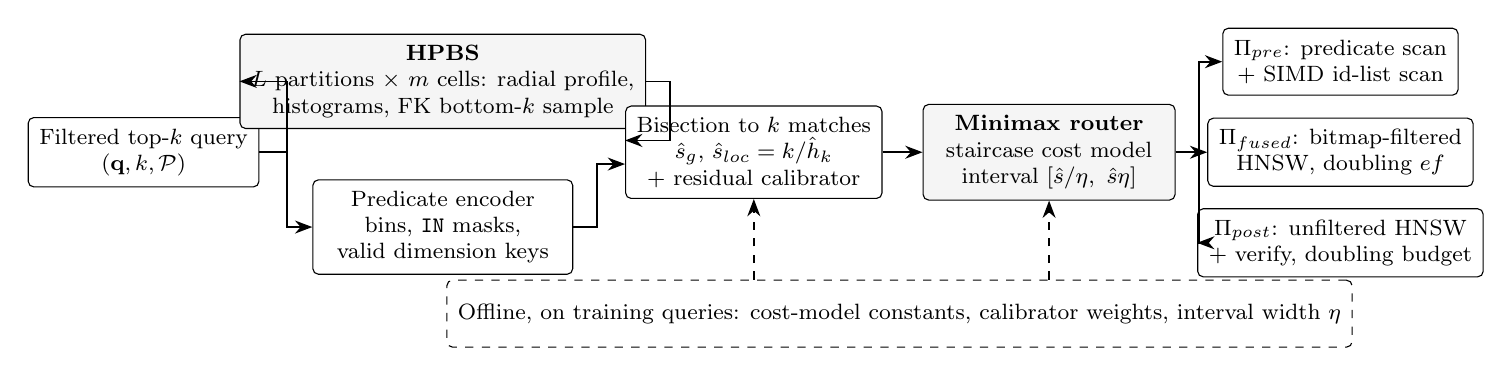
\begin{tikzpicture}[
  font=\footnotesize,
  box/.style={draw, rounded corners=2pt, align=center, minimum height=0.85cm, inner sep=4pt, fill=white},
  graybox/.style={draw, rounded corners=2pt, align=center, minimum height=0.85cm, inner sep=4pt, fill=gray!8},
  dashedbox/.style={draw, dashed, rounded corners=2pt, align=center, minimum height=0.85cm, inner sep=4pt, fill=white},
  arr/.style={-{Stealth[length=2.2mm]}, semithick},
  darr/.style={-{Stealth[length=2.2mm]}, dashed, semithick}
]
\node[box, minimum width=2.2cm] (query) at (0.1, 0.4) {Filtered top-$k$ query\\$(\mathbf{q}, k, \mathcal{P})$};
\node[graybox, minimum width=3.3cm] (sketch) at (3.9, 1.3) {\textbf{HPBS}\\$L$ partitions $\times$ $m$ cells: radial profile,\\histograms, FK bottom-$k$ sample};
\node[box, minimum width=3.3cm] (rel) at (3.9, -0.55) {Predicate encoder\\bins, \texttt{IN} masks,\\valid dimension keys};
\node[box, minimum width=2.9cm] (cal) at (7.85, 0.4) {Bisection to $k$ matches\\$\hat s_g$, $\hat s_{\text{loc}}=k/\hat h_k$\\+ residual calibrator};
\node[graybox, minimum width=3.2cm] (cost) at (11.6, 0.4) {\textbf{Minimax router}\\staircase cost model\\interval $[\hat s/\eta,\ \hat s\eta]$};
\node[box, minimum width=2.6cm] (pre) at (15.3, 1.55) {$\Ppre$: predicate scan\\+ SIMD id-list scan};
\node[box, minimum width=2.6cm] (fused) at (15.3, 0.4) {$\Pfus$: bitmap-filtered\\HNSW, doubling $ef$};
\node[box, minimum width=2.6cm] (post) at (15.3, -0.75) {$\Ppost$: unfiltered HNSW\\+ verify, doubling budget};
\node[dashedbox, minimum width=7.5cm] (calib) at (9.7, -1.65) {Offline, on training queries: cost-model constants, calibrator weights, interval width $\eta$};
\draw[arr] (query.east) -- ++(0.35,0) |- (sketch.west);
\draw[arr] (query.east) -- ++(0.35,0) |- (rel.west);
\draw[arr] (sketch.east) -- ++(0.3,0) |- ([yshift=0.15cm]cal.west);
\draw[arr] (rel.east) -- ++(0.3,0) |- ([yshift=-0.15cm]cal.west);
\draw[arr] (cal.east) -- (cost.west);
\draw[arr] (cost.east) -- ++(0.3,0) |- (pre.west);
\draw[arr] (cost.east) -- (fused.west);
\draw[arr] (cost.east) -- ++(0.3,0) |- (post.west);
\draw[darr] (calib.north -| cost.south) -- (cost.south);
\draw[darr] (calib.north -| cal.south) -- (cal.south);
\end{tikzpicture}
\caption{Architecture of HVO. Planning reads only the sketch, never the vector index. The router evaluates a calibrated cost model at both ends of the estimator's uncertainty interval and runs the plan with the smallest worst-case cost.}
\label{fig:arch}
\end{figure*}

\section{The Polytope-Ball Sketch}\label{sec:sketch}
HPBS answers the question \emph{``how many tuples lie in the ball around $\mathbf{q}$ that holds $k$ matches of $\mathcal{P}$?''} The ball is a region in $\mathbb{R}^d$; the predicate is an axis-aligned polytope in attribute space joined through foreign keys. Space-partitioning trees degrade to scans for $d\gtrsim 30$, and the predicate is not known until query time, so we summarize both sides per cell of a coarse vector partition.

\subsection{Structure}
\emph{Partitions.} We build $L$ independent $k$-means partitions with $m$ cells each, trained on a $2\times10^5$-vector sample with different seeds. For cell $b$ we keep its centroid $\mathbf{c}_b$, its size $N_b$, and a \emph{radial profile}: the $16$ quantiles $\{\rho_{b,j}\}$ of the squared member-to-centroid distances $\|\mathbf{x}-\mathbf{c}_b\|^2$.

\emph{Attribute histograms.} For each numeric attribute we fix $B=32$ global equi-depth bins and store, per cell, the cumulative fraction of the cell's tuples below each bin edge (FP16). For integer-valued attributes (years, counts) the edges are moved to half-integers and an inclusive range $[l,u]$ is read as $[\lceil l\rceil-\tfrac12,\lfloor u\rfloor+\tfrac12]$. Without this, tied values make equi-depth edges collapse; a first run on real data produced P99 Q-errors above $10^4$ for exactly this reason. For each categorical attribute we store per-cell value fractions. A range predicate is answered by linear interpolation inside its two boundary bins; an \texttt{IN} list sums the selected fractions.

\emph{Foreign-key samples.} For each foreign key, a cell stores its $k_{\text{kmv}}=64$ distinct keys with the smallest hash values together with the number of the cell's rows carrying each key. At query time the dimension predicate is evaluated on the (small) dimension table to obtain the valid key set $\mathcal{V}$. The cell's semi-join selectivity is estimated as
\begin{equation}\label{eq:kmv_join}
\hat\sigma^{\text{join}}_b = \frac{\sum_{h\in\mathcal{K}_b} f_b(h)\,\mathbb{I}[h\in\mathcal{V}]}{\sum_{h\in\mathcal{K}_b} f_b(h)},
\end{equation}
a ratio estimator over a uniform hash-sample of the cell's distinct keys that weights each key by its row count. Because $\mathcal{V}$ is materialized exactly, no threshold alignment between two bottom-$k$ sketches is needed. The estimator is consistent but not unbiased, and its variance grows with key skew.

\emph{Cell predicate fraction.} Within a cell we assume the constraints are independent: $\hat\sigma_b = \prod_j \hat\sigma^{(j)}_b \cdot \hat\sigma^{\text{join}}_b$. Correlation \emph{across} cells, which is the spatial-relational correlation that defeats global estimators, is captured by the partition; only the within-cell residual is assumed away.

\emph{Why $k$-means and not random projections.} Our original design used structured cross-polytope LSH cells ($2d_{\text{proj}}$ cones $\times$ $8$ radial shells). Its cells follow random directions rather than the data, so a cell mixes unrelated neighborhoods. In our experiments it is the least accurate variant (P99 Q-error $\QHpbsCpPnnA$ against $\QHpbsPnnA$ for $k$-means cells at $L=4$; Table~\ref{tab:cardinality}).

\subsection{Estimation}
Let $\delta_b=\|\mathbf{q}-\mathbf{c}_b\|^2$. For high-dimensional data the offset of a member from its centroid is nearly orthogonal to $\mathbf{q}-\mathbf{c}_b$, so $\|\mathbf{q}-\mathbf{x}\|^2\approx\delta_b+\|\mathbf{x}-\mathbf{c}_b\|^2$. The estimated number of the cell's tuples inside the ball of squared radius $r$ is therefore
\begin{equation}\label{eq:ballcount}
\hat n_b(r) = \frac{N_b}{16}\,\big|\{j : \delta_b + \rho_{b,j} \le r\}\big|.
\end{equation}
The estimated matches inside the ball are $\hat M(r)=\sum_b \hat n_b(r)\hat\sigma_b$. We find $\hat r$ with $\hat M(\hat r)=k$ by bisection (26 steps), and return
\begin{equation}\label{eq:sloc_hat}
\hat s^{(\ell)}_{\text{loc}} = \min\!\Big(1,\ \frac{k}{\sum_b \hat n_b(\hat r)}\Big), \qquad \hat s_g^{(\ell)} = \frac{1}{N}\sum_b N_b\hat\sigma_b .
\end{equation}
The sketch returns the median over the $L$ partitions. Algorithm~\ref{alg:hpbs} gives the procedure. Each partition costs one $m\times d$ matrix-vector product (Accelerate \texttt{sgemv}), $m$ cell-fraction evaluations, and a bisection whose candidate set shrinks as the upper radius falls, giving $\mathcal{O}(L(md + m|\mathcal{P}| + m\log(1/\epsilon)))$ time.

\begin{table}[!t]
\footnotesize
\centering
\caption{Algorithm 1: HPBS query-time estimation (one partition; the sketch returns the median over $L$).}
\label{alg:hpbs}
\begin{tabular}{p{0.95\columnwidth}}
\toprule
\textbf{Input:} $\mathbf{q}$, $k$, predicate $\mathcal{P}$, partition $\{\mathbf{c}_b, N_b, \rho_{b,\cdot}, \text{hist}_b, \mathcal{K}_b\}_{b=1}^m$.\\
1: Encode $\mathcal{P}$: boundary bins and offsets of each range, bitmask of each \texttt{IN} list, valid key set $\mathcal{V}$ of the dimension predicate.\\
2: $\boldsymbol{\delta}\leftarrow \|\mathbf{c}\|^2 - 2\,\mathbf{C}\mathbf{q} + 1$ \hfill $\triangleright$ one \texttt{sgemv}\\
3: \textbf{for} each cell $b$: $\hat\sigma_b\leftarrow\prod_j\hat\sigma_b^{(j)}\cdot\hat\sigma_b^{\text{join}}$ (Eq.~\eqref{eq:kmv_join}); $\hat s_g \mathrel{+}= N_b\hat\sigma_b/N$.\\
4: $\mathcal{C}\leftarrow\{b:\hat\sigma_b>0\}$; $lo\leftarrow0$; $hi\leftarrow\max_{b\in\mathcal{C}}\delta_b+\rho_{b,16}$.\\
5: \textbf{repeat} 26 times: $r\leftarrow(lo+hi)/2$; \textbf{if} $\sum_{b\in\mathcal{C}}\hat n_b(r)\hat\sigma_b<k$ \textbf{then} $lo\leftarrow r$ \textbf{else} $hi\leftarrow r$; $\mathcal{C}\leftarrow\{b\in\mathcal{C}:\delta_b\le hi\}$.\\
6: \textbf{return} $\hat s_g$, $\hat s_{\text{loc}}\leftarrow\min(1, k/\sum_b\hat n_b(hi))$.\\
\bottomrule
\end{tabular}
\end{table}

\subsection{Residual calibrator}
The raw estimate is biased where the orthogonality approximation in Eq.~\eqref{eq:ballcount} is poor (the query lies close to a centroid) and where within-cell independence fails. A two-layer MLP $f_\Theta:\mathbb{R}^{12}\to\mathbb{R}$ with 16 ReLU units per layer ($\CalParamsA$ parameters) predicts the log-residual, and $\hat s_{\text{loc}}\leftarrow\operatorname{clip}(\hat s^{\text{raw}}_{\text{loc}}e^{f_\Theta(\mathbf{z})},k/N,1)$. The twelve features are: $\ln\hat s_g$; $\ln\hat s^{\text{raw}}_{\text{loc}}$; the variance and the range of $\ln\hat s^{(\ell)}_{\text{loc}}$ across partitions; the number of predicate terms; a join indicator; the number of range terms; the number of \texttt{IN} terms; the log of the mean number of active cells; the mean and the standard deviation across partitions of the bisection radius $\hat r$; and $\ln\hat s^{\text{raw}}_{\text{loc}}-\ln\hat s_g$. It is trained on the training split only, with squared log-error, $L_2$ penalty $10^{-3}$ and early stopping. Its forward pass takes about $\CalUsA\,\mu$s in NumPy.

\subsection{Error decomposition}\label{sec:errdecomp}
Let $n_b(r)$ and $M_b(r)$ be the true numbers of tuples and of matches of cell $b$ inside the ball of squared radius $r$, and $\sigma_b(r)=M_b(r)/n_b(r)$. Write $h(j)$ for the number of tuples within the distance of the $j$-th closest match, so $h_k=h(k)$.
\begin{proposition}[Deterministic error decomposition]\label{prop:decomp}
Suppose that for every $r$ and $b$ the geometric and cell estimates satisfy
\[
\hat n_b(r)\in\big[n_b(r)/\alpha,\ \alpha n_b(r)\big],\qquad \hat\sigma_b\in\big[\sigma_b(r)/\beta,\ \beta\sigma_b(r)\big].
\]
Then
\[
\text{Q-error}(\hat s_{\text{loc}}, \sloc) \le \alpha\cdot\psi(\alpha\beta), \quad \psi(t)=\max\Big(\frac{h(\lceil tk\rceil)}{h(k)},\ \frac{h(k)}{h(\lfloor k/t\rfloor)}\Big).
\]
If matches are locally uniform around $\mathbf{q}$ ($h(j)\propto j$), then $\psi(t)\approx t$ and the Q-error is at most $\alpha^2\beta$.
\end{proposition}
\begin{proof}
With $M(r)=\sum_b n_b(r)\sigma_b(r)$,
\[
\hat M(r)=\textstyle\sum_b\hat n_b\hat\sigma_b\in\big[M(r)/(\alpha\beta),\ \alpha\beta M(r)\big].
\]
At the bisection point $\hat M(\hat r)=k$, so $M(\hat r)$ lies in $[k/(\alpha\beta),\ \alpha\beta k]$. Since $M$ and $n=\sum_b n_b$ are non-decreasing in $r$,
\[
n(\hat r)\in\big[h(\lfloor k/(\alpha\beta)\rfloor),\ h(\lceil\alpha\beta k\rceil)\big].
\] Finally $\sum_b\hat n_b(\hat r)\in[n(\hat r)/\alpha,\ \alpha n(\hat r)]$, and $\hat s_{\text{loc}}/\sloc = h(k)/\sum_b\hat n_b(\hat r)$.
\end{proof}
\emph{What the parameters control.} Smaller cells (larger $m$) and a finer radial profile reduce $\alpha$; larger $B$ and $k_{\text{kmv}}$ reduce the histogram and join parts of $\beta$. The remaining part of $\beta$ is within-cell spatial-relational correlation, and $\psi$ depends on how matches are arranged around $\mathbf{q}$. Neither is controlled by the sketch's parameters. We therefore make no distribution-free accuracy claim: Proposition~\ref{prop:decomp} explains where error comes from, and Section~\ref{sec:eval_card} measures it. We prove nothing about the calibrator.

\emph{Space and maintenance.} HPBS stores $Lm(d+16)$ floats for centroids and profiles, $Lm\sum_j B_j$ FP16 histogram entries, and $Lm k_{\text{kmv}}$ key--count pairs, independent of $N$ apart from the choice of $m$. With $L=4$, $m=1024$ it takes $\QHpbsMBA$, $\QHpbsMBC$ and $\QHpbsMBB$\,MiB for 128-, 384- and 768-d vectors ($\SketchPctA\%$, $\SketchPctC\%$ and $\SketchPctB\%$ of the raw vectors), dominated by the centroids. It is built in $\BuildHpbsA$--$\BuildHpbsB$\,s, against $\BuildHnswA$--$\BuildHnswB$\,s for the HNSW index on 10 threads. Insertions update one cell per partition (counts, histogram entries, and a bottom-$k$ insertion). Deletions can be handled by decrementing counts and dropping key entries, with lazy cell rebuilds. We have not evaluated maintenance under updates.

\section{Plans and Hardware-Calibrated Cost Model}\label{sec:routing}
\subsection{Plans}
All plans are implemented on faiss~\cite{douze2024faiss} \texttt{IndexHNSWFlat} (inner product, $M=32$, $ef_{\text{construction}}=200$) and run single-threaded.
\begin{itemize}
    \item $\Ppre$ evaluates $\mathcal{P}$ column-wise over all $N$ rows (NumPy), takes the sorted id list, and runs a C top-$k$ scan over the listed rows. The scan prefetches whole rows ahead and comes in three kernels: scalar FP32 (auto-vectorization disabled), NEON FP32 ($4\times4$ FMA accumulators), and NEON INT8 (\texttt{SDOT} on symmetric int8 codes for the top $4k$, followed by an exact FP32 rerank).
    \item $\Ppost$ searches the unfiltered graph with budget $e$ (search queue and result list of size $e$), verifies $\mathcal{P}$ on the candidates, and doubles $e$ from $64$ until $k$ matches are found, up to $2^{17}$. Restarting rounds instead of resuming costs at most a factor of about two over a resumable implementation.
    \item $\Pfus$ materializes $\mathcal{P}$ as a bitmap and passes it to faiss's HNSW search as an \texttt{IDSelectorBitmap}, so non-matching nodes are traversed but never returned. It doubles $ef$ from $64$ until $k$ results are found \emph{and} a doubled budget returns the same set. We added the second condition after observing recall of $0.23$ at $\sloc<1\%$ when stopping at the first $k$ results.
\end{itemize}
Because the plans adapt their budgets, a plan's latency does not depend on the optimizer's estimate; the optimizer only chooses which plan runs. This makes the oracle well defined.

\subsection{Cost model}
\emph{Staircase plans.} A graph plan whose rounds have budgets $e_i=e_0 2^i$ and which stops once the budget reaches a need $\nu$ runs $j(\nu)=\lceil\log_2(\nu/e_0)\rceil^+$ rounds, capped at the budget limit. If a round of budget $e$ costs $b_0+b_1e^\gamma$, the plan costs
\begin{equation}\label{eq:stair}
\operatorname{St}(\nu;b_0,b_1,\gamma)=\sum_{i=0}^{j(\nu)}\big(b_0+b_1(e_02^i)^\gamma\big).
\end{equation}
\emph{Plan costs.} With $C_{\text{rel}}=c_0+c_1N|\mathcal{P}|+c_2N\,\mathbb{I}[\text{join}]$ for columnar predicate evaluation,
\begin{align}
C(\Ppre)&=C_{\text{rel}}+a_0+c_{\text{scan}}\,\sg N,\label{eq:cost_pre}\\
C(\Ppost)&=\operatorname{St}\!\big(k/\sloc;\,\theta_{\text{post}}\big),\label{eq:cost_post}\\
C(\Pfus)&=C_{\text{rel}}+\operatorname{St}^{+1}\!\big(c_f(k/\sloc)^{\beta_f};\,\theta_{\text{fused}}\big),\label{eq:cost_fused}
\end{align}
where $\operatorname{St}^{+1}$ adds the confirmation round. The need of $\Ppost$ is exactly $h_k=k/\sloc$ (Definition~\ref{def:sloc}). Filtered traversal needs a budget that grows faster than $h_k$, which we capture with $\beta_f$.

\emph{Calibration.} The constants are fitted on the training queries using their \emph{true} selectivities and measured latencies: $(c_0,c_1,c_2)$ and $(a_0,c_{\text{scan}})$ by non-negative least squares on relative error, and $\theta$ by nonlinear least squares in log space ($\gamma\in[0.3,2.5]$, with $c_f$ and $\beta_f$ chosen on a grid). On SYN-128 the fit gives $c_1=\RelNsA$\,ns per row and predicate term and $c_{\text{scan}}=\ScanSimdA$\,ns per vector for the NEON kernel. It also gives $\gamma_{\text{post}}=\PostGammaA$, $\gamma_{\text{fused}}=\FusedGammaA$, and $\beta_f=\FusedBetaA$. The superlinear $\gamma$ is a property of faiss's HNSW search: its candidate queue makes large budgets disproportionately expensive. One round at $e=65{,}536$ cost about $2$\,s on SYN-128. A first model that assumed $\gamma\le1$, as the analysis of the original draft did, underpredicted the cost of fused plans by up to $10\times$ and misrouted tail queries even when given the true selectivities.

\emph{Hardware-agnostic ablation.} To isolate the hardware calibration we also fit the same staircases to \emph{distance-evaluation counts} instead of time, so that a sequential and a random distance computation cost the same, as in cost models that count distance evaluations.

\subsection{Phase boundary}
\begin{theorem}[Pre-filter boundary]\label{thm:crossover}
Let $C_G(\sloc)$ denote the cost of the cheaper graph plan, $\min(C(\Pfus),C(\Ppost))$. Under the cost model of Eqs.~\eqref{eq:cost_pre} to~\eqref{eq:cost_fused}, the pre-filter plan is optimal if and only if
\[
\sg\le\sg^*(\sloc)=\frac{C_G(\sloc)-C_{\text{rel}}-a_0}{c_{\text{scan}}N}.
\]
If $C_G(\sloc)<C_{\text{rel}}+a_0$, $\Ppre$ is never optimal. Holding the other terms fixed, replacing a scan kernel by one that is $\lambda$ times faster multiplies $\sg^*$ by $\lambda$.
\end{theorem}
\begin{proof}
$C(\Ppre)$ is affine and increasing in $\sg$, and $C_G$ does not depend on $\sg$; equate and solve. The scaling follows because $c_{\text{scan}}$ enters only in the denominator.
\end{proof}
Theorem~\ref{thm:crossover} has a consequence that matters in practice. When predicates are evaluated by scanning columns, $C_{\text{rel}}$ is linear in $N$, so pre-filtering pays $\Theta(N)$ even for very selective predicates. For local selectivities above roughly $1$--$2\%$, a graph plan is then cheaper whatever $\sg$ is. The boundary becomes nearly a horizontal line in the $(\sg,\sloc)$ plane, and global selectivity carries little information about the right plan (Figure~\ref{fig:phase}). The kernel enters through $c_{\text{scan}}$, which on SYN-128 is $\ScanScalarA$, $\ScanSimdA$, and $\ScanIEightA$\,ns per vector for the scalar, NEON FP32 and INT8 kernels.

\begin{figure}[!t]
\centering
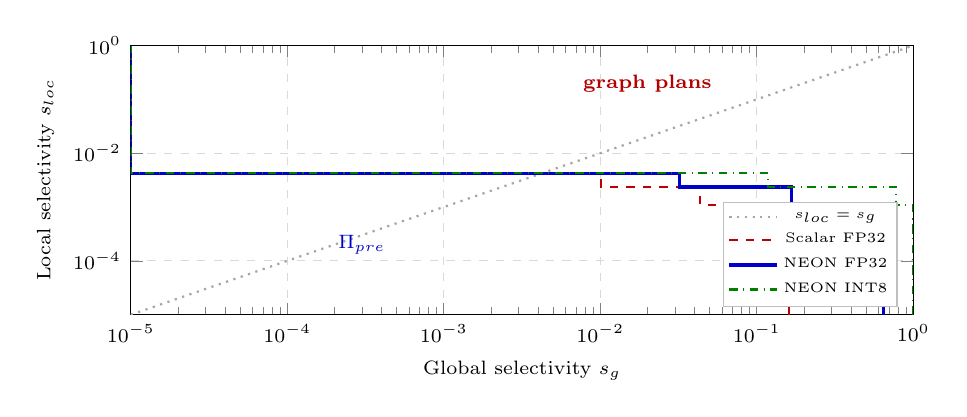
\begin{tikzpicture}
\begin{axis}[
    width=0.95\columnwidth, height=5.0cm,
    xmode=log, ymode=log,
    xmin=1e-5, xmax=1, ymin=1e-5, ymax=1,
    xlabel={Global selectivity $s_g$}, ylabel={Local selectivity $s_{\text{loc}}$},
    xlabel style={font=\scriptsize}, ylabel style={font=\scriptsize},
    ticklabel style={font=\scriptsize},
    legend style={at={(0.98,0.03)}, anchor=south east, font=\tiny, draw=gray!50, fill=white, inner sep=1.5pt},
    grid=major, grid style={dashed, gray!30}
]
\addplot[gray!70, dotted, thick, domain=1e-5:1, samples=2] {x};
\addplot[red!75!black, dashed, thick, const plot] coordinates {\phaseScalarA};
\addplot[blue!80!black, very thick, const plot] coordinates {\phaseSimdA};
\addplot[green!50!black, dashdotted, thick, const plot] coordinates {\phaseIEightA};
\node[font=\scriptsize\bfseries, blue!80!black, align=center] at (axis cs:3e-4,2e-4) {$\Pi_{\text{pre}}$};
\node[font=\scriptsize\bfseries, red!70!black, align=center] at (axis cs:2e-2,0.2) {graph plans};
\legend{$s_{\text{loc}}=s_g$, Scalar FP32, NEON FP32, NEON INT8}
\end{axis}
\end{tikzpicture}
\caption{Pre-filter boundary $s_g^*(s_{\text{loc}})$ of Theorem~\ref{thm:crossover} on SYN-128 for the three scan kernels (cost model calibrated on the training split; two predicate terms, no join). Below and to the left of each curve pre-filtering is cheapest. Faster kernels push the boundary to larger $s_g$. Above $s_{\text{loc}}\approx1\%$ a graph plan wins for every $s_g$, because columnar predicate evaluation already costs $\Theta(N)$.}
\label{fig:phase}
\end{figure}

\subsection{Routing}
\emph{Point routing} picks $\arg\min_\Pi C(\Pi;\hat s_g,\hat s_{\text{loc}})$. \emph{Minimax routing} uses an interval $I=[\hat s_{\text{loc}}/\eta,\ \hat s_{\text{loc}}\eta]$ and picks
\begin{equation}\label{eq:robust}
\begin{aligned}
\hat\Pi&=\arg\min_\Pi\ \max_{s\in I}C(\Pi;\hat s_g,s)\\
&=\arg\min_\Pi\ \max\big(C(\Pi;\hat s_g,\hat s_{\text{loc}}/\eta),\ C(\Pi;\hat s_g,\hat s_{\text{loc}}\eta)\big),
\end{aligned}
\end{equation}
since every plan cost is monotone in $\sloc$. We set $\eta$ to the $0.9$-quantile of the estimator's Q-error on the training split, fixed before looking at test data ($\eta=\EtaHvoA$ and $\EtaHvoB$ for HPBS). Because $C(\Ppre)$ does not depend on $\sloc$, minimax routing prefers the plan whose cost is certain whenever the estimate is uncertain.

\emph{Runtime guard.} We also evaluated an early-exit rule that aborts $\Ppost$ after its first round if the observed match rate is below half the estimate and the cost model predicts $\Ppre$ to be cheaper than the remaining rounds. It is replayed exactly from the recorded per-round timings.

\section{Regret Analysis}\label{sec:theory}
Regret is $\mathcal{R}=C(\hat\Pi;s)/C(\Pi^*;s)$, where $\Pi^*$ minimizes cost at the true selectivities $s=(\sg,\sloc)$. The results below concern the cost model of Section~\ref{sec:routing}. Measured regret differs from model regret by the model's calibration error, which we report in Section~\ref{sec:eval}. All statements hold per query, given that query's estimation error.

\begin{lemma}[Sensitivity of staircase plans]\label{lem:sens}
Let a plan's cost be $A+\operatorname{St}(c\,(k/s)^\beta;b_0,b_1,\gamma)$ with $A,b_0,b_1\ge0$ and $\gamma>0$. If $\hat s/s\in[1/\eta,\eta]$, then its cost at $\hat s$ is within a factor $\Lambda_{\beta,\gamma}(\eta)$ of its cost at $s$, where
\[
\Lambda_{\beta,\gamma}(\eta)=1+\delta\,2^{\gamma\delta},\qquad \delta=\lceil\beta\log_2\eta\rceil .
\]
\end{lemma}
\begin{proof}
The needs differ by a factor of at most $\eta^\beta$, so the round counts differ by at most $\delta$, because $\lceil x+y\rceil\le\lceil x\rceil+\lceil y\rceil$. Suppose the larger cost has $j+\delta$ rounds and the smaller $j$ (fewer additional rounds only shrink the ratio). The constant parts have ratio $(j+\delta+1)/(j+1)\le1+\delta$. With $r=2^\gamma$ the geometric parts have ratio
\[
\frac{\sum_{i\le j+\delta}r^i}{\sum_{i\le j}r^i}=1+\frac{r^{j+1}}{\sum_{i\le j}r^i}\sum_{i<\delta}r^i\le1+r\sum_{i<\delta}r^{i}\le1+\delta r^{\delta},
\]
using $\sum_{i\le j}r^i\ge r^j$ and $r\ge1$. A ratio of sums is at most the largest ratio of its parts, and adding $A\ge0$ to both costs only decreases the ratio. Capping the round count at the budget limit also only decreases it.
\end{proof}
The factor is $1$ when $\eta<2^{1/\beta}$ \emph{and} no doubling boundary lies between the two needs. In the worst case, though, an arbitrarily small error can cross a boundary, which costs one extra round and gives the factor $1+2^\gamma$. This discreteness is a real property of adaptive plans, not an artifact of the proof.

Let $\Lambda=\max(\eta_g,\Lambda_{1,\gamma_{\text{post}}}(\eta),\Lambda_{\beta_f,\gamma_{\text{fused}}}(\eta))$, where $\eta_g$ bounds the multiplicative error of $\hat s_g$, which enters $C(\Ppre)$ affinely.

\begin{theorem}[Point routing]\label{thm:regret}
If $\hat s_g/\sg\in[1/\eta_g,\eta_g]$ and also $\hat s_{\text{loc}}/\sloc\in[1/\eta,\eta]$, then point routing has $\mathcal{R}\le\Lambda^2$. If, in addition, $\hat s_g=\sg$ and either $\hat\Pi$ or $\Pi^*$ is $\Ppre$, then $\mathcal{R}\le\Lambda$.
\end{theorem}
\begin{proof}
By Lemma~\ref{lem:sens}, $C(\Pi;\hat s)\in[C(\Pi;s)/\Lambda,\ \Lambda C(\Pi;s)]$ for every plan. Hence $C(\hat\Pi;s)\le\Lambda C(\hat\Pi;\hat s)\le\Lambda C(\Pi^*;\hat s)\le\Lambda^2C(\Pi^*;s)$. If $\hat\Pi=\Ppre$ and its cost is exact, the first factor is $1$. If $\Pi^*=\Ppre$, the last factor is $1$.
\end{proof}

\begin{theorem}[Minimax routing]\label{thm:robust}
Suppose $\hat s_g=\sg$ and $\sloc\in I=[\hat s_{\text{loc}}/\eta,\hat s_{\text{loc}}\eta]$. Then minimax routing (Eq.~\eqref{eq:robust}) satisfies: (i) if $\Pi^*=\Ppre$, then $\mathcal{R}=1$; (ii) in all cases $\mathcal{R}\le\Lambda(\eta^2)$.
\end{theorem}
\begin{proof}
Let $\bar C(\Pi)=\max_{s'\in I}C(\Pi;s')$; since $\sloc\in I$, $C(\Pi;s)\le\bar C(\Pi)$. (i) $C(\Ppre)$ does not depend on $\sloc$, so $\bar C(\Ppre)=C(\Ppre;s)$, and $C(\hat\Pi;s)\le\bar C(\hat\Pi)\le\bar C(\Ppre)=C(\Pi^*;s)$. (ii) $C(\hat\Pi;s)\le\bar C(\hat\Pi)\le\bar C(\Pi^*)\le\Lambda(\eta^2)C(\Pi^*;s)$, because any $s'\in I$ is within a factor $\eta^2$ of $\sloc$.
\end{proof}
Theorem~\ref{thm:robust} is the formal reason for minimax routing. Misrouting a query whose best plan is the exact pre-filter scan to a graph plan is the failure that produces the worst tail latencies: the graph plan can be orders of magnitude slower. Minimax routing provably avoids it whenever the interval covers the truth. The price is conservatism: when the interval is wide, the router may scan where a graph plan would have been faster.

\begin{proposition}[Global-selectivity routing]\label{prop:unbounded}
Let a router choose its plan as any function of $\sg$ alone. Let graph-plan costs satisfy $C_G(1)\le C_1$ and $C_G(k/N)\ge bN^\gamma$ for constants $C_1,b,\gamma>0$, and let $C(\Ppre)=a+c'\sg N$, which holds when predicates are evaluated through an index at a cost proportional to their output. Then for $N$ large enough that $k\le\sqrt{bN^\gamma C_1/c'}$, its worst-case regret over instances with that $N$ is at least $\sqrt{bN^\gamma/(c'C_1)}\,/\,(1+o(1))$, that is, $\Omega(N^{\gamma/2})$.
\end{proposition}
\begin{proof}
Fix $s^*=\sqrt{bN^\gamma C_1/c'}/N\ge k/N$. Matching tuples can be placed around $\mathbf{q}$ ($\sloc=1$) or beyond all non-matching tuples ($\sloc=k/N$) while keeping $\sg=s^*$, and the router cannot tell the two instances apart. If it picks $\Ppre$, the first instance gives $\mathcal{R}\ge c's^*N/C_1$. If it picks a graph plan, the second gives $\mathcal{R}\ge bN^\gamma/(a+c's^*N)$. Both equal $\sqrt{bN^\gamma/(c'C_1)}$ up to the lower-order term $a$.
\end{proof}
With columnar predicate evaluation, $C(\Ppre)\ge c_1N$ for every $\sg$. The same argument then gives regret $\Omega(\min(N, N^{\gamma-1}))$. This is a constant set by the ratio of random-access to per-row predicate cost when $\gamma\le1$, and it still grows with $N$ for the superlinear $\gamma$ we measure. HVO's bounds, by contrast, depend only on the estimation error. This contrast is why we measure the estimator's tail and not only its median.

\section{Experimental Evaluation}\label{sec:eval}
We ask four questions. How accurate and how fast is HPBS, compared with histogram, exact-count, sampling and index-probing estimators (Section~\ref{sec:eval_card})? Does better estimation translate into lower end-to-end latency (Section~\ref{sec:eval_e2e})? How do the scan kernel and each component matter (Section~\ref{sec:eval_hw})? And how does measured regret compare with the bounds (Section~\ref{sec:eval_regret})?

\subsection{Setup}\label{sec:setup}
\emph{Hardware and software.} Apple M4 (4 performance and 6 efficiency cores, 16\,GB unified memory), macOS, Python~3.14, NumPy (Accelerate BLAS), faiss-cpu~1.13.2, Apple clang with \texttt{-O3 -mcpu=native}. All latencies are measured on one thread (OpenMP and Accelerate both limited to one thread). Each plan is run once as a warm-up and then twice; we report the slower of the two timed runs. A first run of the 768-d benchmark was invalidated because two copies of the vectors (table and index) exceeded memory and the machine swapped. In the reported runs the table aliases the index's vector storage. We logged swap activity every minute: the remaining swap-ins came from other processes paging in, and the timed process stayed CPU-bound (above $85\%$ CPU utilization whenever we checked).

\emph{Synthetic data.} Each synthetic benchmark has $N=10^6$ unit-norm vectors from a two-level mixture (64 topics $\times$ 16 subtopics with Zipfian popularity) in $d=128$ (SYN-128) or $d=768$ (SYN-768). Attributes are generated from the latent topic with graded correlation. \texttt{category} (32 values) equals the topic's value with probability $0.7$; \texttt{lang} (12 values) follows the subtopic with probability $0.5$; \texttt{year} has a topic-specific mean plus Gaussian noise; \texttt{rating} has a weak subtopic effect; \texttt{price} (log-normal) and \texttt{views} (Pareto) are independent of the vectors. A foreign key references a 20{,}000-row seller table with \texttt{region} (10 values) and \texttt{tier} (4 values). For $60\%$ of rows the seller is drawn, with Zipfian popularity, from the topic's preferred region.

\emph{Real data (ARXIV-384).} We sample $10^6$ papers, plus a disjoint pool of $3000$ query papers, from the CC0-licensed arXiv-abstracts-2021 dump (about $2\times10^6$ papers)~\cite{arxivdump}. Each paper is embedded with the sentence encoder all-MiniLM-L6-v2~\cite{reimers2019sbert} ($d=384$, title and abstract truncated to the model's 128-token training length, unit norm). All attributes are real metadata:
\begin{itemize}
    \item \texttt{archive}: the top-level archive of the primary category (31 archives plus ``other'');
    \item \texttt{published}: whether the paper has a journal reference;
    \item \texttt{year}: the submission year, taken from the identifier (1991--2021);
    \item \texttt{n\_cats}: the number of listed categories;
    \item \texttt{n\_authors} and \texttt{abs\_words}: the author count and abstract length.
\end{itemize}
A foreign key references a dimension table of the 172 primary categories, with their subject \texttt{group} (8 values: physics, mathematics, computer science, \ldots) and a popularity quartile. Spatial-relational correlation is not injected here: it arises because a paper's text determines both its embedding and its field.

\emph{Queries.} On synthetic data a query vector is a data vector plus Gaussian noise of norm about $0.35$, renormalized; on ARXIV-384 it is the embedding of a held-out paper. Its predicate is a conjunction of 1--3 terms drawn independently of the vector: numeric ranges of random width $2$--$90\%$ of the quantile range, \texttt{IN} lists, and semi-joins on the two dimension attributes. Because predicates are drawn independently of the query, correlation arises naturally: a \texttt{category} or \texttt{archive} filter either includes or excludes the query's topic or field. We generate $1000$ training and $1500$ test queries per benchmark from disjoint seeds and drop queries with no match. The test splits contain $\nAntiA/\nIndepA/\nPosA$ (SYN-128), $\nAntiB/\nIndepB/\nPosB$ (SYN-768) and $\nAntiC/\nIndepC/\nPosC$ (ARXIV-384) anti-correlated/independent/positively correlated queries. They include $\nRareA$, $\nRareB$ and $\nRareC$ queries with $\sloc<10^{-3}$; real data has far more of them. Ground truth (exact $\sg$, $h_k$, and filtered top-$10$) comes from brute force. Everything fitted---the calibrator, the cost model, the thresholds of the global routers, and the interval width $\eta$---uses only the training split.

\emph{Baselines.} The estimators are:
\begin{itemize}
    \item \emph{1-D histograms + AVI} (PostgreSQL-style): 100 equi-depth bins per continuous column and exact value frequencies for categorical and integer-valued columns (as most-common-value lists would give), independence across terms, a uniform foreign-key assumption, and $\hat s_{\text{loc}}=\hat s_g$.
    \item \emph{Exact $s_g$ + AVI} (Milvus-style): the exact predicate count, with $\hat s_{\text{loc}}=\sg$.
    \item \emph{1\% uniform sample}: the rank of the first sampled match among sampled tuples.
    \item \emph{HNSW probe} (Exqutor-style): the match rate among the first 256 unfiltered neighbors returned by the index ($ef=256$).
\end{itemize}
Each is fed to the same cost model, with point and with minimax routing. The routers additionally include the three static plans and global-selectivity routers with two-way ($\Ppre$/$\Ppost$) and three-way thresholds on the exact $\sg$, tuned on the training split to minimize mean latency (which is generous to them). We do not run \texttt{pgvector}, Milvus, DuckDB or ACORN themselves: these policies isolate the routing decision on identical plan implementations.

\emph{Metrics.} The oracle runs all three plans and picks the fastest with Recall@10$\ge0.9$; the other routers are charged their plan's latency plus their planning time. Measured regret is the ratio of a router's latency to the oracle's. Plan accuracy is agreement with the oracle's choice, which penalizes near-ties, so we emphasize latency and regret.

\begin{table*}[!t]
\footnotesize
\renewcommand{\arraystretch}{0.95}
\centering
\caption{Local-selectivity Q-error on the test split, by correlation regime and for rare local matches ($\sloc<10^{-3}$), and median planning-time cost of the estimator. Lower is better.}
\label{tab:cardinality}
\setlength{\tabcolsep}{4.2pt}
\begin{tabular}{lccccccccccc}
\toprule
 & \multicolumn{3}{c}{Anti-correlated} & \multicolumn{3}{c}{Independent} & \multicolumn{3}{c}{Positively correlated} & Rare & Time \\
\cmidrule(lr){2-4}\cmidrule(lr){5-7}\cmidrule(lr){8-10}
Estimator & P50 & P95 & P99 & P50 & P95 & P99 & P50 & P95 & P99 & P99 & ($\mu$s) \\
\midrule
\csname @@input\endcsname generated/card_rows.tex
\bottomrule
\end{tabular}
\end{table*}

\subsection{Selectivity estimation}\label{sec:eval_card}
Table~\ref{tab:cardinality} and Figure~\ref{fig:card} report Q-error on the test split.

\emph{Independence-based estimators fail under correlation.} Both histogram-based AVI and exact-count AVI reach P99 Q-errors of $\QPgHistPnnA$ and $\QExactAviPnnA$ on SYN-128. Their errors are concentrated in the anti-correlated regime and grow sharply for rare local matches ($\QPgHistRareA$ and $\QExactAviRareA$). Knowing $\sg$ exactly does not help, because the error is in assuming $\sloc=\sg$. The exact count also costs $\QExactAviUsA\,\mu$s, because it evaluates the predicate over all rows during planning.

\emph{Sampling starves.} The 1\% sample (P99 $\QSampleOnePnnA$) bases its estimate on very few sampled matches near the query and is noisy across all regimes.

\emph{Index probing is accurate on average but fails on rare matches.} The HNSW probe is the strongest baseline (P99 $\QProbePnnA$ and $\QProbePnnB$). When no match appears among the first 256 neighbors it can only report an upper bound, so its rare-match P99 is $\QProbeRareA$ and $\QProbeRareB$. It also costs $\QProbeUsA$ and $\QProbeUsB\,\mu$s of random index accesses.

\emph{Real data is harder.} On ARXIV-384 the tails are an order of magnitude heavier for every estimator. Text determines both a paper's embedding and its field, so correlation is strong: exact-count AVI reaches a P99 Q-error of $\QExactAviPnnC$ and histograms $\QPgHistPnnC$. The HNSW probe's P99 rises to $\QProbePnnC$ and $\QProbeRareC$ on rare matches. The calibrated sketch reaches $\QHpbsPlusCalPnnC$ ($\QHpbsPlusCalRareC$ on rare matches), the best of all estimators, and the 1\% sample is second ($\QSampleOnePnnC$), at a memory footprint of about 15\,MiB and $\QSampleOneUsC\,\mu$s per estimate.

\emph{HPBS.} The calibrated sketch has the lowest P99 Q-error on every benchmark ($\QHpbsPlusCalPnnA$, $\QHpbsPlusCalPnnB$ and $\QHpbsPlusCalPnnC$), and it stays the most accurate on rare local matches ($\QHpbsPlusCalRareA$, $\QHpbsPlusCalRareB$ and $\QHpbsPlusCalRareC$). That is the regime where index probing and histograms are least accurate and where misrouting is most expensive. The raw sketch is already accurate at the median and on rare matches. The calibrator mainly removes its tail, reducing the P99 from $\QHpbsPnnA$ to $\QHpbsPlusCalPnnA$ on SYN-128 and from $\QHpbsPnnC$ to $\QHpbsPlusCalPnnC$ on ARXIV-384. One partition ($L=1$) is almost as accurate after calibration ($\QHpbsLOnePlusCalPnnA$ and $\QHpbsLOnePlusCalPnnB$) at $\PlanShareLOneA\%$ and $\PlanShareLOneB\%$ of the planning time. HPBS is less accurate than the probe at the median for well-populated neighborhoods; its advantage lies in the tail.

\begin{figure*}[!t]
\centering
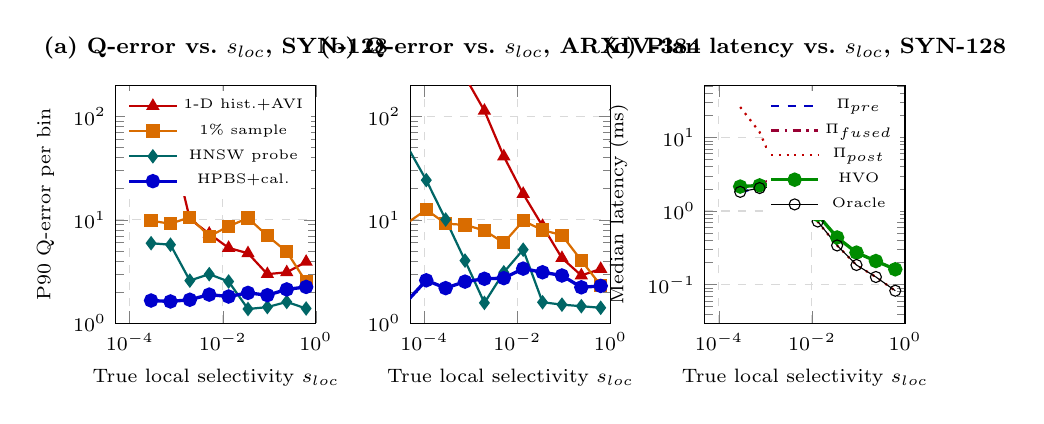
\begin{tikzpicture}
\begin{axis}[
    name=q1, width=0.34\textwidth, height=4.6cm,
    xmode=log, ymode=log, xmin=5e-5, xmax=1, ymin=1, ymax=200,
    xlabel={True local selectivity $s_{\text{loc}}$}, ylabel={P90 Q-error per bin},
    xlabel style={font=\scriptsize}, ylabel style={font=\scriptsize}, ticklabel style={font=\scriptsize},
    title style={font=\footnotesize\bfseries}, title={(a) Q-error vs.\ $s_{\text{loc}}$, SYN-128},
    legend style={at={(0.98,0.98)}, anchor=north east, font=\tiny, draw=none, fill=white, inner sep=1pt},
    grid=major, grid style={dashed, gray!30}]
\addplot[red!75!black, mark=triangle*, thick] coordinates {\binqPgHistA};
\addplot[orange!85!black, mark=square*, thick] coordinates {\binqSampleOneA};
\addplot[teal!80!black, mark=diamond*, thick] coordinates {\binqProbeA};
\addplot[blue!80!black, mark=*, very thick] coordinates {\binqHpbsPlusCalA};
\legend{1-D hist.+AVI, 1\% sample, HNSW probe, HPBS+cal.}
\end{axis}
\begin{axis}[
    name=q2, at={(q1.east)}, anchor=west, xshift=1.2cm, width=0.34\textwidth, height=4.6cm,
    xmode=log, ymode=log, xmin=5e-5, xmax=1, ymin=1, ymax=200,
    xlabel={True local selectivity $s_{\text{loc}}$},
    xlabel style={font=\scriptsize}, ticklabel style={font=\scriptsize},
    title style={font=\footnotesize\bfseries}, title={(b) Q-error vs.\ $s_{\text{loc}}$, ARXIV-384},
    grid=major, grid style={dashed, gray!30}]
\addplot[red!75!black, mark=triangle*, thick] coordinates {\binqPgHistC};
\addplot[orange!85!black, mark=square*, thick] coordinates {\binqSampleOneC};
\addplot[teal!80!black, mark=diamond*, thick] coordinates {\binqProbeC};
\addplot[blue!80!black, mark=*, very thick] coordinates {\binqHpbsPlusCalC};
\end{axis}
\begin{axis}[
    name=q3, at={(q2.east)}, anchor=west, xshift=1.2cm, width=0.34\textwidth, height=4.6cm,
    xmode=log, ymode=log, xmin=5e-5, xmax=1, ymin=0.03,
    xlabel={True local selectivity $s_{\text{loc}}$}, ylabel={Median latency (ms)},
    xlabel style={font=\scriptsize}, ylabel style={font=\scriptsize}, ticklabel style={font=\scriptsize},
    title style={font=\footnotesize\bfseries}, title={(c) Plan latency vs.\ $s_{\text{loc}}$, SYN-128},
    legend style={at={(0.98,0.98)}, anchor=north east, font=\tiny, draw=none, fill=white, inner sep=1pt},
    grid=major, grid style={dashed, gray!30}]
\addplot[blue!75!black, thick, dashed] coordinates {\binpreA};
\addplot[purple!80!black, thick, dashdotted] coordinates {\binfusedA};
\addplot[red!75!black, thick, dotted] coordinates {\binpostA};
\addplot[green!55!black, very thick, mark=*] coordinates {\binhvoA};
\addplot[black, thin, mark=o] coordinates {\binoracleA};
\legend{$\Pi_{\text{pre}}$, $\Pi_{\text{fused}}$, $\Pi_{\text{post}}$, HVO, Oracle}
\end{axis}
\end{tikzpicture}
\caption{(a, b) P90 Q-error within bins of true local selectivity: the baselines degrade as matches become rare near the query, and HPBS does not. (c) Median latency of each plan by true local selectivity on SYN-128, with HVO (including planning time) and the oracle. Pre-filtering is flat in $s_{\text{loc}}$; the graph plans' cost explodes as $s_{\text{loc}}$ falls.}
\label{fig:card}
\end{figure*}

\begin{table*}[!t]
\footnotesize
\renewcommand{\arraystretch}{0.94}
\centering
\caption{End-to-end latency (ms, including planning time), recall, plan accuracy against the oracle, measured regret, and median planning time ($\mu$s) on the test split. CM: the calibrated cost model of Section~\ref{sec:routing}. ``Robust'' denotes minimax routing with the interval width fitted on the training split.}
\label{tab:e2e}
\setlength{\tabcolsep}{4.6pt}
\begin{tabular}{lccccccccc}
\toprule
Router & Mean & P50 & P95 & P99 & Recall@10 & Plan acc.\ (\%) & Mean regret & P99 regret & Plan ($\mu$s) \\
\midrule
\csname @@input\endcsname generated/e2e_rows.tex
\bottomrule
\end{tabular}
\end{table*}

\subsection{End-to-end routing}\label{sec:eval_e2e}
Table~\ref{tab:e2e} reports latency, recall and regret for every router, and Figure~\ref{fig:card}(c) shows where the plans cross.

\emph{No static plan is acceptable.} Pre-filtering always pays the full predicate scan (mean $\RAlwaysPreMeanA$\,ms on SYN-128). Post-filtering is the best plan for most queries, but its P99 is $\RAlwaysPostPnnA$\,ms because anti-correlated queries force it through a large part of the graph. Static fused traversal is worse still, because filtered traversal without two-hop expansion loses connectivity at low $\sloc$.

\emph{Global-selectivity routing has a large regret tail.} Tuned two-way thresholds give a mean of $\RGlobalTwoWayMeanA$\,ms and $\RGlobalTwoWayMeanB$\,ms with P99 regret $\RGlobalTwoWayRegPnnA$ and $\RGlobalTwoWayRegPnnB$. Every query above the threshold goes to post-filtering regardless of $\sloc$, as Proposition~\ref{prop:unbounded} predicts. The three-way variant finds no profitable fused band on SYN-128, where its thresholds collapse to the two-way rule. On SYN-768 it lowers the mean to $\RGlobalThreeWayMeanB$\,ms. Its regret tail stays large.

\emph{Correlation-blind estimates poison a good cost model.} Feeding the same cost model with histogram or exact-count AVI estimates is worse than the simple threshold (mean $\RCboPgHistMeanA$ and $\RCboExactAviMeanA$\,ms): the model trusts $\hat s_{\text{loc}}=\sg$ and sends anti-correlated queries to graph plans.

\emph{HVO.} With HPBS estimates and minimax routing, HVO has a mean latency of $\RHvoMeanA$\,ms and $\RHvoMeanB$\,ms. That is $\MeanGainVsGlobalA\%$ and $\MeanGainVsGlobalB\%$ below the best tuned global router ($\RBestGlobalMeanA$ and $\RBestGlobalMeanB$\,ms) and close to the oracle ($\ROracleMeanA$ and $\ROracleMeanB$\,ms). On SYN-768 it matches the cost model fed the \emph{true} selectivities ($\RCboTrueMeanB$\,ms), so estimation is no longer the bottleneck there. Its P99 regret is $\RHvoRegPnnA$ and $\RHvoRegPnnB$, against $\RGlobalTwoWayRegPnnA$ and $\RGlobalTwoWayRegPnnB$ for the two-way router. On the synthetic benchmarks HVO does \emph{not} improve P99 latency over the two-way threshold rule ($\RHvoPnnA$ vs.\ $\RGlobalTwoWayPnnA$\,ms on SYN-128, $\RHvoPnnB$ vs.\ $\RGlobalTwoWayPnnB$\,ms on SYN-768). That rule sends many queries to the pre-filter scan, whose cost is bounded, so its slowest queries are no slower than a scan; it pays for this in the mean. HVO's tail consists of graph plans that the cost model priced correctly on average but that run long for individual queries. Point routing with the same estimates has a similar mean but a much heavier latency tail ($\RHvoPointPnnA$\,ms P99 on SYN-128). That is the failure Theorem~\ref{thm:robust} rules out. The probe-based cost model is the strongest competitor. With minimax routing it comes within a few percent of HVO ($\RRobProbeMeanA$ vs.\ $\RHvoMeanA$\,ms), because both estimators are accurate where most queries lie. HVO's advantage is that it never touches the vector index during planning and that it remains accurate on rare local matches.

\emph{Real data.} On ARXIV-384 the gap between routers widens, because local selectivity there often differs from global selectivity by orders of magnitude:
\begin{itemize}
    \item \emph{Correlation-blind estimates are catastrophic.} The cost model fed exact-count AVI estimates averages $\RCboExactAviMeanC$\,ms, because it sends anti-correlated queries into graph plans that traverse most of the graph.
    \item \emph{Global thresholds are a poor fit.} The best tuned global router averages $\RBestGlobalMeanC$\,ms.
    \item \emph{HVO.} It averages $\RHvoMeanC$\,ms, close to the cost model fed true selectivities ($\RCboTrueMeanC$\,ms) and to the oracle ($\ROracleMeanC$\,ms). Unlike on the synthetic benchmarks, its P99 latency ($\RHvoPnnC$\,ms) is also below the threshold rule's ($\RGlobalTwoWayPnnC$\,ms) and close to the oracle's ($\ROraclePnnC$\,ms); its P99 regret is $\RHvoRegPnnC$, against $\RGlobalTwoWayRegPnnC$.
    \item \emph{Index probing.} The probe-based cost model is again the closest competitor ($\RCboProbeMeanC$\,ms, $\RRobProbeMeanC$\,ms with minimax routing). Its tail estimation errors cost it more here than on synthetic data.
    \item \emph{One partition.} With $L=1$, HVO averages $\RHvoLOneMeanC$\,ms: at real-data latencies, the planning time saved outweighs the small loss in accuracy.
\end{itemize}

\emph{What limits HVO.} Three factors account for the rest of the gap to the oracle:
\begin{itemize}
    \item \emph{Planning time.} Excluding it, HVO's choices reach $\RHvoNoplanMeanA$ and $\RHvoNoplanMeanB$\,ms. At $\RHvoUsA$ and $\RHvoUsB\,\mu$s, planning matters when the best plan itself takes a few hundred microseconds. Roughly a third of it is Python orchestration around the C kernel.
    \item \emph{Cost-model calibration.} For the best plan the model's error is median $\kappa_{\text{cal}}=\KappaMedA$ (P95 $\KappaPnfA$) on SYN-128 and $\KappaMedB$ (P95 $\KappaPnfB$) on SYN-768.
    \item \emph{Recall.} The oracle only accepts plans with Recall@10 $\ge 0.9$, while the routers' graph plans occasionally return fewer true neighbors. Their mean recall is $\RHvoRecA$ and $\RHvoRecB$ against $\ROracleRecA$ and $\ROracleRecB$ for the oracle. A recall-aware cost model is future work.
\end{itemize}

\subsection{Hardware kernels and ablations}\label{sec:eval_hw}
\begin{table}[!t]
\footnotesize
\renewcommand{\arraystretch}{0.94}
\centering
\caption{Scan kernel sensitivity. $c_{\text{scan}}$: fitted cost per scanned vector. $s_g^*$ (\%): pre-filter boundary at $s_{\text{loc}}=0.3\%$ and $1\%$ for two predicate terms (Theorem~\ref{thm:crossover}; 100 means pre-filtering wins for every $s_g$, 0 that it never does). \#pre: queries for which the oracle / HVO choose $\Pi_{\text{pre}}$. Latencies in ms.}
\label{tab:hw}
\setlength{\tabcolsep}{2.6pt}
\resizebox{\columnwidth}{!}{%
\begin{tabular}{llcccccccc}
\toprule
Data & Kernel & $c_{\text{scan}}$ (ns) & $s_g^*$@0.3\% & $s_g^*$@1\% & \#pre opt & \#pre HVO & HVO mean & HVO P99 & Oracle mean \\
\midrule
\csname @@input\endcsname generated/hw_rows.tex
\bottomrule
\end{tabular}}
\end{table}

\emph{Scan kernels.} Table~\ref{tab:hw} repeats routing with each pre-filter kernel. The NEON FP32 kernel is $\ScanRatioA\times$ (SYN-128) and $\ScanRatioB\times$ (SYN-768) cheaper per vector than the scalar kernel, and INT8 \texttt{SDOT} with FP32 rerank is another $\ScanRatioIEightA\times$ and $\ScanRatioIEightB\times$ cheaper. Faster kernels widen the pre-filter region (Figure~\ref{fig:phase}), and the oracle picks $\Ppre$ more often. The calibrated cost model follows the shift, because only $c_{\text{scan}}$ changes.

\emph{Component ablations.} Table~\ref{tab:ablation} removes one component at a time:
\begin{itemize}
    \item \emph{Hardware-agnostic cost.} Replacing time-calibrated costs by distance-evaluation counts makes sequential and random distance computations cost the same. HVO's mean rises from $\RHvoMeanA$ to $\RHvoAgnosticMeanA$\,ms on SYN-128 and from $\RHvoMeanC$ to $\RHvoAgnosticMeanC$\,ms on ARXIV-384.
    \item \emph{Calibrator.} Without it, the raw sketch's heavier tail forces a wider interval ($\eta$ from the raw estimator's training Q-error), and minimax routing becomes overly conservative.
    \item \emph{Interval width.} Widths between the $0.75$- and $0.95$-quantiles perform similarly; the $0.99$-quantile scans too often.
    \item \emph{Runtime guard.} The early-exit guard fired on $\FiredA$, $\FiredB$ and $\FiredC$ test queries (SYN-128, SYN-768, ARXIV-384) and slightly \emph{increased} mean latency. Its triggers come from the first, smallest round, where a low observed match rate is weak evidence. We report it as a negative result.
\end{itemize}

\begin{table*}[!t]
\footnotesize
\renewcommand{\arraystretch}{0.94}
\centering
\caption{Ablations of HVO: mean and P99 latency (ms), plan accuracy (\%), and P99 measured regret.}
\label{tab:ablation}
\setlength{\tabcolsep}{4.0pt}
\begin{tabular}{lcccccccccccc}
\toprule
 & \multicolumn{4}{c}{SYN-128} & \multicolumn{4}{c}{SYN-768} & \multicolumn{4}{c}{ARXIV-384 (real)} \\
\cmidrule(lr){2-5}\cmidrule(lr){6-9}\cmidrule(lr){10-13}
Variant & Mean & P99 & Acc. & P99 reg. & Mean & P99 & Acc. & P99 reg. & Mean & P99 & Acc. & P99 reg. \\
\midrule
\csname @@input\endcsname generated/abl_rows.tex
\bottomrule
\end{tabular}
\end{table*}

\subsection{Regret versus estimation error}\label{sec:eval_regret}
To test Theorems~\ref{thm:regret} and~\ref{thm:robust}, we replace the estimate by $\hat s_{\text{loc}}=\sloc\,\eta^{\pm1}$ with a random sign (an adversarial, interval-endpoint error), keep $\hat s_g=\sg$, and route the SYN-128 test queries 20 times per value of $\eta$ (Figure~\ref{fig:regret}). Across $\NoiseChecksA$ routed queries the model regret never exceeded the bound of Lemma~\ref{lem:sens} and Theorems~\ref{thm:regret}--\ref{thm:robust} ($\NoiseViolTotalA$ violations). Minimax routing had zero regret on every query whose best plan was $\Ppre$.

The bounds are loose. With the measured $\gamma_{\text{fused}}=\FusedGammaA$, a single extra doubling round costs a factor $1+2^{\gamma}\approx\NoiseBoundOnePOneA$, which is the bound already at $\eta=1.1$, while the observed P99 model regret is $\NoiseModelOnePOneA$. The figure also shows the cost of conservatism. When every estimate sits at an endpoint of its interval, minimax routing is more conservative than point routing (P99 model regret $\NoiseRobustTwoPZeroA$ vs.\ $\NoiseModelTwoPZeroA$ at $\eta=2$). Under HPBS's actual error distribution, where most errors are small and a few are large, it removes the latency tail (Table~\ref{tab:e2e}).

\begin{figure}[!t]
\centering
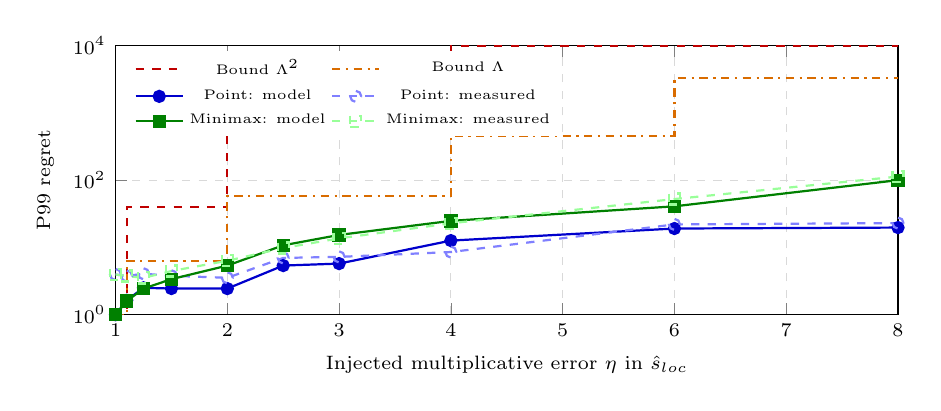
\begin{tikzpicture}
\begin{axis}[
    width=0.95\columnwidth, height=5.0cm,
    xmin=1, xmax=8, ymode=log, ymin=1, ymax=1e4,
    xlabel={Injected multiplicative error $\eta$ in $\hat s_{\text{loc}}$}, ylabel={P99 regret},
    xlabel style={font=\scriptsize}, ylabel style={font=\scriptsize}, ticklabel style={font=\scriptsize},
    legend style={at={(0.02,0.98)}, anchor=north west, font=\tiny, draw=none, fill=white, inner sep=1pt, legend columns=2},
    grid=major, grid style={dashed, gray!30}]
\addplot[red!75!black, thick, dashed, const plot] coordinates {\noiseboundgeneral};
\addplot[orange!85!black, thick, dashdotted, const plot] coordinates {\noiseboundtight};
\addplot[blue!80!black, mark=*, thick] coordinates {\noisemodel};
\addplot[blue!50, mark=o, thick, dashed] coordinates {\noisemeasured};
\addplot[green!50!black, mark=square*, thick] coordinates {\noiserobustmodel};
\addplot[green!40, mark=square, thick, dashed] coordinates {\noiserobustmeasured};
\legend{Bound $\Lambda^2$, Bound $\Lambda$, Point: model, Point: measured, Minimax: model, Minimax: measured}
\end{axis}
\end{tikzpicture}
\caption{Regret on SYN-128 under injected estimation error ($\hat s_g=s_g$; 20 repetitions). Model regret uses the calibrated cost model at the true selectivities; measured regret uses the executed plans' latencies and includes the cost model's calibration error, which is why it exceeds 1 even at $\eta=1$. Bounds are clipped at $10^4$.}
\label{fig:regret}
\end{figure}

\section{Discussion and Limitations}\label{sec:discussion}
\emph{Data.} We have one real dataset. Its embeddings and metadata are real, but its predicates, like those of the synthetic benchmarks, are drawn at random rather than taken from a query log. The two synthetic benchmarks control correlation but share one generator. HVO's advantage was \emph{larger} on real data than on synthetic data, which suggests the synthetic correlation is milder than real correlation. A second real domain (for example product catalogs or multimodal embeddings) and a real query workload would test this further.

\emph{One machine, one library.} Absolute latencies and the fitted constants are specific to an Apple M4 and faiss's HNSW. The cost model's structure (staircases, a per-vector scan cost, a per-row predicate cost) carries over, but its constants must be recalibrated per machine, and the superlinear round cost we measure is a property of faiss's search implementation rather than of HNSW in general. We do not compare against \texttt{pgvector}, Milvus, DuckDB or ACORN as systems. Our global-selectivity routers reproduce their \emph{routing policies} on identical plans, which isolates the optimizer from engine differences but does not measure those engines.

\emph{Planning overhead.} HPBS's query path is C, but the predicate encoding and median-of-$L$ logic are Python. At hundreds of microseconds of planning time against sub-millisecond plans, this matters. A fully native implementation inside a DBMS planner hook would reduce it, and $L=1$ already cuts it by half or more at a small loss in tail accuracy.

\emph{Not evaluated.} We have not evaluated updates, \texttt{GROUP BY} top-$k$ (which changes the post-filtering horizon from $k$ matches to $k$ distinct groups), multi-way joins, two-hop fused traversal as in ACORN, or skewed foreign keys stress-tested in isolation. Higher-order attribute correlation inside a cell is not modeled.

\section{Conclusion}
Choosing a plan for filtered vector search requires knowing how far the search must travel before it meets $k$ matches, and that distance is a local, correlation-dependent quantity. HVO estimates it with a compact sketch that never touches the index, prices plans with a cost model calibrated on the target hardware, and routes with a minimax rule that provably avoids the most expensive class of misroutes. On one million real arXiv papers, HPBS is the most accurate estimator in the tail and on rare local matches, and HVO lowers mean latency by $\MeanGainVsGlobalC\%$ relative to tuned global-selectivity routing, with tail latency close to an oracle's. On two synthetic benchmarks the mean-latency gains are smaller ($\MeanGainVsGlobalA\%$ and $\MeanGainVsGlobalB\%$), and there HVO does not beat the threshold rule's P99 latency. Its recall is slightly below the oracle's on all three. The results come from one machine and plans built on faiss; validating them inside a production planner and on real query workloads is future work.

\section*{Declarations and Reproducibility}
\noindent\textbf{Funding and conflicts of interest:} This research received no external funding. The authors declare no conflicts of interest.\\
\textbf{Code and data:} Implementation, data generator, experiment drivers, raw results and the scripts that generate every number, table and figure in this paper are available at \url{https://github.com/sanmish4ds/HyperVectorOptimizer}.\\
\textbf{Author contributions:} \textbf{S. Mishra:} conceptualization, methodology, formal analysis, software, writing (original draft). \textbf{D. Chukkapalli:} validation, investigation, visualization, writing (review and editing).

\begin{thebibliography}{99}

\bibitem{wei2020analyticdbv}
C.~Wei \emph{et al.}, ``AnalyticDB-V: A hybrid analytical engine towards query fusion for structured and unstructured data,'' \emph{Proc. VLDB Endow.}, vol.~13, no.~12, pp.~3152--3165, 2020.

\bibitem{zhang2023vbase}
Q.~Zhang \emph{et al.}, ``VBase: Unifying online vector similarity search and relational queries via relaxed monotonicity,'' in \emph{Proc. USENIX OSDI}, 2023, pp.~377--395.

\bibitem{patel2024acorn}
L.~Patel, P.~Kraft, C.~Guestrin, and M.~Zaharia, ``ACORN: Performant and predicate-agnostic search over vector embeddings and structured data,'' \emph{Proc. ACM Manag. Data}, vol.~2, no.~3, 2024.

\bibitem{amanbayev2026fanns}
A.~Amanbayev, B.~Tsan, T.~Dang, and F.~Rusu, ``Filtered approximate nearest neighbor search in vector databases: System design and performance analysis,'' arXiv:2602.11443, 2026.

\bibitem{lin2025survey}
Y.~Lin, K.~Zhang, Z.~He, Y.~Jing, and X.~S.~Wang, ``Survey of filtered approximate nearest neighbor search over the vector-scalar hybrid data,'' arXiv:2505.06501, 2025.

\bibitem{iff2025benchmark}
P.~Iff \emph{et al.}, ``Benchmarking filtered approximate nearest neighbor search algorithms on transformer-based embedding vectors,'' arXiv:2507.21989, 2025.

\bibitem{shi2025unified}
J.~Shi, Y.~Cai, and W.~Zheng, ``Filtered approximate nearest neighbor search: A unified benchmark and systematic experimental study,'' arXiv:2509.07789, 2025.

\bibitem{pgvector2024}
A.~Kane, ``pgvector: Open-source vector similarity search for Postgres,'' 2024. [Online]. Available: \url{https://github.com/pgvector/pgvector}

\bibitem{duckdbvss2024}
DuckDB, ``Vector similarity search extension (\texttt{vss}),'' 2024. [Online]. Available: \url{https://duckdb.org/docs/extensions/vss}

\bibitem{wang2021milvus}
J.~Wang \emph{et al.}, ``Milvus: A purpose-built vector data management system,'' in \emph{Proc. ACM SIGMOD}, 2021, pp.~2614--2627.

\bibitem{malkov2018hnsw}
Y.~A. Malkov and D.~A. Yashunin, ``Efficient and robust approximate nearest neighbor search using hierarchical navigable small world graphs,'' \emph{IEEE Trans. Pattern Anal. Mach. Intell.}, vol.~42, no.~4, pp.~824--836, 2020.

\bibitem{douze2024faiss}
M.~Douze \emph{et al.}, ``The Faiss library,'' arXiv:2401.08281, 2024.

\bibitem{gollapudi2023filtereddiskann}
S.~Gollapudi \emph{et al.}, ``Filtered-DiskANN: Graph algorithms for approximate nearest neighbor search with filters,'' in \emph{Proc. ACM Web Conf.}, 2023, pp.~3406--3416.

\bibitem{wang2022nhq}
M.~Wang, L.~Lv, X.~Xu, Y.~Wang, Q.~Yue, and J.~Ni, ``Navigable proximity graph-driven native hybrid queries with structured and unstructured constraints,'' arXiv:2203.13601, 2022.

\bibitem{wu2022hqann}
W.~Wu \emph{et al.}, ``HQANN: Efficient and robust similarity search for hybrid queries with structured and unstructured constraints,'' in \emph{Proc. ACM CIKM}, 2022, pp.~4580--4584.

\bibitem{zuo2024serf}
C.~Zuo, M.~Qiao, W.~Zhou, F.~Li, and D.~Deng, ``SeRF: Segment graph for range-filtering approximate nearest neighbor search,'' \emph{Proc. ACM Manag. Data}, vol.~2, no.~1, 2024.

\bibitem{peng2025drfanns}
Z.~Peng, M.~Qiao, W.~Zhou, F.~Li, and D.~Deng, ``Dynamic range-filtering approximate nearest neighbor search,'' \emph{Proc. VLDB Endow.}, vol.~18, no.~10, pp.~3256--3268, 2025.

\bibitem{exqutor2026}
H.~Kim, C.~Lim, H.~An, R.~Sen, and K.~Park, ``Exqutor: Extended query optimizer for vector-augmented analytical queries,'' arXiv:2512.09695, 2025.

\bibitem{selinger1979systemr}
P.~G. Selinger \emph{et al.}, ``Access path selection in a relational database management system,'' in \emph{Proc. ACM SIGMOD}, 1979, pp.~23--34.

\bibitem{matias1998wavelet}
Y.~Matias, J.~S. Vitter, and M.~Wang, ``Wavelet-based histograms for selectivity estimation,'' in \emph{Proc. ACM SIGMOD}, 1998, pp.~448--459.

\bibitem{gunopulos2000approximating}
D.~Gunopulos, G.~Kollios, V.~J. Tsotras, and C.~Domeniconi, ``Approximating multi-dimensional aggregate range queries over real attributes,'' in \emph{Proc. ACM SIGMOD}, 2000, pp.~463--474.

\bibitem{flajolet2007hll}
P.~Flajolet, {\'E}.~Fusy, O.~Gandouet, and F.~Meunier, ``HyperLogLog: The analysis of a near-optimal cardinality estimation algorithm,'' in \emph{Proc. AofA}, 2007, pp.~127--146.

\bibitem{beyer2007kmv}
K.~Beyer, P.~J. Haas, B.~Reinwald, Y.~Sismanis, and R.~Gemulla, ``On synopses for distinct-value estimation under multiset operations,'' in \emph{Proc. ACM SIGMOD}, 2007, pp.~199--210.

\bibitem{kipf2019mscn}
A.~Kipf \emph{et al.}, ``Learned cardinalities: Estimating correlated joins with deep learning,'' in \emph{Proc. CIDR}, 2019.

\bibitem{yang2020neurocard}
Z.~Yang \emph{et al.}, ``NeuroCard: One cardinality estimator for all tables,'' \emph{Proc. VLDB Endow.}, vol.~14, no.~1, pp.~61--73, 2020.

\bibitem{hilprecht2020deepdb}
B.~Hilprecht, A.~Schmidt, M.~Kulessa, A.~Molina, K.~Kersting, and C.~Binnig, ``DeepDB: Learn from data, not from queries!'' \emph{Proc. VLDB Endow.}, vol.~13, no.~7, pp.~992--1005, 2020.

\bibitem{charikar2002similarity}
M.~S. Charikar, ``Similarity estimation techniques from rounding algorithms,'' in \emph{Proc. ACM STOC}, 2002, pp.~380--388.

\bibitem{spring2017new}
R.~Spring and A.~Shrivastava, ``A new unbiased and efficient class of LSH-based samplers and estimators for partition function computation in log-linear models,'' arXiv:1703.05160, 2017.

\bibitem{lan2024cardinality}
H.~Lan, S.~Huang, Z.~Bao, and R.~Borovica-Gajic, ``Cardinality estimation for similarity search on high-dimensional data objects: The impact of reference objects,'' \emph{Proc. VLDB Endow.}, vol.~18, no.~3, pp.~544--556, 2024.

\bibitem{arxivdump}
``arxiv-abstracts-2021: metadata and abstracts of arXiv papers,'' Hugging Face dataset \texttt{gfissore/arxiv-abstracts-2021}, CC0 license, 2021. [Online]. Available: \url{https://huggingface.co/datasets/gfissore/arxiv-abstracts-2021}

\bibitem{reimers2019sbert}
N.~Reimers and I.~Gurevych, ``Sentence-BERT: Sentence embeddings using Siamese BERT-networks,'' in \emph{Proc. EMNLP-IJCNLP}, 2019, pp.~3982--3992.

\end{thebibliography}

\end{document}
